
\documentclass[12pt,oneside,openany]{report}

% ============================================================
% 1. CONFIGURACIÓN DE IDIOMA Y CODIFICACIÓN
% ============================================================

\usepackage[spanish,es-tabla]{babel}
\usepackage[utf8]{inputenc}
\usepackage[T1]{fontenc}
\usepackage{lmodern}

% ============================================================
% 2. CONFIGURACIÓN DE PÁGINA
% ============================================================

\usepackage[
    letterpaper,
    margin=2.54cm,
    headheight=15pt
]{geometry}

\usepackage{graphicx}
\usepackage{microtype}
\usepackage{setspace}
\usepackage{fancyhdr}
\usepackage{titlesec}
\usepackage{placeins}
\usepackage{pdflscape}
\usepackage{amsmath}
\usepackage{xurl}

% ============================================================
% 3. TABLAS, FIGURAS Y ELEMENTOS GRÁFICOS
% ============================================================

\usepackage{
    booktabs,
    tabularx,
    longtable,
    array
}

\usepackage{float}
\usepackage[table]{xcolor}
\usepackage{caption}
\usepackage{chngcntr}
\usepackage[table]{xcolor}
\usepackage{tocloft}
\usepackage{amsmath}
\usepackage{amssymb}

% ============================================================
% 4. ENLACES Y REFERENCIAS CRUZADAS
% ============================================================

\usepackage{hyperref}
\usepackage{cleveref}
\usepackage{url}

% ============================================================
% 5. CÓDIGO FUENTE Y LISTAS
% ============================================================

\usepackage{listings}
\usepackage{enumitem}

% ============================================================
% 6. CITAS Y REFERENCIAS BIBLIOGRÁFICAS - APA 7
% ============================================================

\usepackage{csquotes}

\usepackage[
    backend=biber,
    style=apa,
    sorting=nyt
]{biblatex}

\addbibresource{referencias.bib}

% ============================================================
% 7. COLORES INSTITUCIONALES
% ============================================================

\definecolor{univalle}{HTML}{D90016}
\definecolor{gris}{HTML}{555555}

% ============================================================
% 8. CONFIGURACIÓN DE HIPERVÍNCULOS
% ============================================================

\hypersetup{
    colorlinks=true,
    linkcolor=black,
    citecolor=univalle,
    urlcolor=univalle,
    pdftitle={Rhyzome - Documentación final},
    pdfauthor={Equipo Rhyzome}
}

% ============================================================
% 9. FORMATO GENERAL APA 7
% ============================================================

% Interlineado doble
\doublespacing

% Sangría de primera línea
\setlength{\parindent}{1.27cm}

% Sin espacio adicional entre párrafos
\setlength{\parskip}{0pt}

% ============================================================
% 10. FORMATO DE TÍTULOS Y SUBTÍTULOS
% ============================================================

% Capítulos
\titleformat{\chapter}[hang]
    {\normalfont\bfseries\centering\large}
    {\thechapter.}
    {0.6em}
    {}

\titlespacing*{\chapter}
    {0pt}
    {0pt}
    {12pt}

% Secciones
\titleformat{\section}
    {\normalfont\large\bfseries}
    {\thesection}
    {1em}
    {}

% Subsecciones
\titleformat{\subsection}
    {\normalfont\normalsize\bfseries}
    {\thesubsection}
    {1em}
    {}

% ============================================================
% 11. ENCABEZADOS Y NUMERACIÓN DE PÁGINAS
% ============================================================

\pagestyle{fancy}

\fancyhf{}

% Número de página en la esquina superior derecha
\fancyhead[R]{\thepage}

% Eliminar línea horizontal del encabezado
\renewcommand{\headrulewidth}{0pt}

% Estilo de páginas iniciales de capítulos
\fancypagestyle{plain}{
    \fancyhf{}
    \fancyhead[R]{\thepage}
    \renewcommand{\headrulewidth}{0pt}
}

% ============================================================
% 12. FORMATO DE FIGURAS Y TABLAS
% ============================================================

\captionsetup{
    font=normalsize,
    labelfont=bf,
    justification=raggedright,
    singlelinecheck=false
}

% Numeración consecutiva de figuras
\renewcommand{\thefigure}{\arabic{figure}}

% Numeración consecutiva de tablas
\renewcommand{\thetable}{\arabic{table}}

% Evitar reiniciar numeración por capítulo
\counterwithout{figure}{chapter}
\counterwithout{table}{chapter}

% ------------------------------------------------------------
% Formato del índice de tablas
% ------------------------------------------------------------

\renewcommand{\cfttabpresnum}{Tabla~}
\renewcommand{\cfttabaftersnum}{.}
\setlength{\cfttabnumwidth}{2.5cm}
\setlength{\cfttabindent}{0cm}

% ------------------------------------------------------------
% Formato del índice de figuras
% ------------------------------------------------------------

\renewcommand{\cftfigpresnum}{Figura~}
\renewcommand{\cftfigaftersnum}{.}
\setlength{\cftfignumwidth}{2.5cm}
\setlength{\cftfigindent}{0cm}

% ============================================================
% 13. COMANDOS PERSONALIZADOS
% ============================================================

% Texto para contenido pendiente
\newcommand{\pendiente}[1]{
    \textcolor{gris}{
        \textit{[Pendiente: #1]}
    }
}

% Inserción de figuras
\newcommand{\insertarfigura}[3]{
    \begin{figure}[htbp]
        \caption{#2}
        \label{#3}

        \centering

        \includegraphics[
            width=.88\textwidth
        ]{#1}
    \end{figure}
}

% ============================================================
% 14. CONFIGURACIÓN DE FRAGMENTOS DE CÓDIGO
% ============================================================

\lstset{
    basicstyle=\ttfamily\small,
    breaklines=true,
    frame=single,
    columns=fullflexible,
    showstringspaces=false
}

% ============================================================
% INICIO DEL DOCUMENTO
% ============================================================

\begin{document}

% ============================================================
% 15. PORTADA INSTITUCIONAL
% ============================================================

\begin{titlepage}

    % Ocultar número de página en la portada
    \thispagestyle{empty}

    \centering

    \vspace*{0.15cm}

    % Logotipo Universidad del Valle
    
\includegraphics[
        width=2.5cm
    ]{imagenes/logo_univalle.jpg}

    \par

    \vspace{0.35cm}

    % Universidad
    {
        \normalsize\bfseries
        UNIVERSIDAD DEL VALLE
        \par
    }

    \vspace{0.15cm}

    % Programa académico
    {
        \normalsize
        MAESTRÍA PARA EL DESARROLLO
        DE APLICACIONES INTELIGENTES
        \par
    }

    \vspace{0.65cm}

    % Asignatura
    {
        \normalsize
        TRABAJO INTEGRADOR 3
        \par
    }

    \vspace{0.35cm}

    % Nombre del proyecto
    {
        \LARGE\bfseries
        Rhyzome
        \par
    }

    \vspace{0.15cm}

    % Subtítulo
    {
        \large
        Generador Procedural de Mapas
        \par
    }

    \vspace{0.35cm}

    % Tipo de documento
    {
        \normalsize\bfseries
        Documentación Final del Proyecto
        \par
    }

    \vspace{0.75cm}

    % Autor
    {
        \normalsize
        Presentado por:
        \par
    }

    {
        Christian Andres Morales Mera
        \par
    }

    \vspace{0.3cm}

    % Asesor
    {
        \normalsize
        Profesor asesor:
        \par
    }

    {
        Deisy Chaves Sanchez
        \par
    }

    \vfill

    % Ciudad y año
    Santiago de Cali, Colombia
    \par

    \the\year

\end{titlepage}

% ============================================================
% 16. NUMERACIÓN DEL DOCUMENTO
% ============================================================

% Numeración arábiga
\pagenumbering{arabic}

% ============================================================
% 17. RESUMEN
% ============================================================

\chapter*{Resumen}

\addcontentsline{toc}{chapter}{Resumen}

{
    El desarrollo de videojuegos requiere la creación de escenarios que permitan ofrecer experiencias variadas y dinámicas a los jugadores. Sin embargo, el diseño manual de mapas puede representar un proceso complejo y demandante en términos  de tiempo y recursos. Este proyecto presenta \textbf{Rhyzome}, una aplicación web orientada a la generación procedural y a técnicas de aprendizaje automático. La solución implementa los algoritmos Perlin Noise y Autómatas Celulares para generar escenarios correspondientes a bosques, desiertos, ciudades y mazmorras. Adicionalmente, incorpora un componente inteligente basado en modelos de clasificación supervisada, cuyo propósito es evaluar las características de los mapas generados y apoyar su selección según niveles de complejidad. La aplicación utiliza Python y Flask para el procesamiento de mapas y React para la interacción con el usuario. El desarrollo se gestiona mediante la metodología ágil Scrum, incorporando  planificación iterativa, pruebas automatizadas y validación funcional. Como resultado, se dispone de un prototipo web que integra generación procedural, evaluación de características y selección asistida por aprendizaje automático, proporcionando una base tecnológica para la creación y experimentación con escenarios bidimensionales.
}

\textbf{Palabras clave:}
generación procedural, videojuegos,
aprendizaje automático, mapas 2D.

\clearpage

% ============================================================
% 18. TABLA DE CONTENIDO
% ============================================================

\tableofcontents

\clearpage

% ============================================================
% 19. ÍNDICE DE FIGURAS
% ============================================================

\listoffigures

\addcontentsline{toc}{chapter}{Índice de figuras}

\clearpage

% ============================================================
% 20. ÍNDICE DE TABLAS
% ============================================================

\listoftables

\addcontentsline{toc}{chapter}{Índice de tablas}

\clearpage

% ============================================================
% 21. CAPÍTULOS DEL PROYECTO RHYZOME
% ============================================================

% Capítulo 1: Información General del Proyecto
\chapter{Información General del Proyecto}
\label{cap:01_informacion_general}

El presente capítulo proporciona una descripción general del proyecto \textbf{Rhyzome}, incluyendo su identificación, propósito, equipo de trabajo, organización de responsabilidades, acompañamiento académico y duración. Esta información permite contextualizar el desarrollo del proyecto y establecer las condiciones generales bajo las cuales se llevó a cabo.

% ============================================================
% 1.1. NOMBRE DEL PROYECTO
% ============================================================

\section{Nombre del proyecto}

El proyecto se denomina \textbf{Rhyzome --- Generador Procedural de Mapas 2D para Videojuegos}.

Rhyzome es una aplicación web orientada a la generación procedural de escenarios bidimensionales para videojuegos, mediante la integración de algoritmos de generación procedural y técnicas de aprendizaje automático (\textbf{Machine Learning}).

La solución permite generar diferentes tipos de escenarios, como bosques, desiertos, ciudades y mazmorras, utilizando algoritmos como Perlin Noise y Autómatas Celulares. Adicionalmente, incorpora un componente inteligente que analiza las características de los mapas generados y apoya su selección de acuerdo con niveles de complejidad definidos.

El proyecto busca proporcionar una herramienta que facilite la creación y experimentación con escenarios bidimensionales, integrando generación procedural, evaluación de características y técnicas de inteligencia artificial.

% ============================================================
% 1.2. EQUIPO DE TRABAJO
% ============================================================

\section{Equipo de trabajo}

El desarrollo de Rhyzome se realiza como un proyecto académico individual en el marco del programa de maestría de la Universidad del Valle.

El equipo de trabajo está conformado por \textbf{Christian Andres Morales  Mera}, responsable de la planificación, diseño, implementación, validación y documentación del sistema.

La ejecución del proyecto comprende actividades relacionadas con el desarrollo de software, la implementación de algoritmos procedurales, la experimentación con modelos de aprendizaje automático y la gestión de actividades mediante prácticas ágiles.

% ============================================================
% 1.3. INTEGRANTES Y ROLES SCRUM
% ============================================================

\section{Integrantes y roles SCRUM}

Para la organización y seguimiento del desarrollo se adoptan prácticas de la metodología  ágil Scrum, adaptadas a las características de un proyecto académico individual.

Debido a que el proyecto cuenta con un único desarrollador, las responsabilidades asociadas a los roles de Scrum se concentran en una misma persona, sin constituir un equipo Scrum tradicional.

La Tabla~\ref{tab:roles_scrum} presenta la
distribución de responsabilidades.


\begin{table}[htbp]
    \centering

    \caption{Roles y responsabilidades en Rhyzome}
    \label{tab:roles_scrum}

    \renewcommand{\arraystretch}{1.5}

    \begin{tabularx}{\textwidth}{
        |>{\raggedright\arraybackslash}p{3cm}|
         >{\raggedright\arraybackslash}X|
    }
        \hline

        \rowcolor{gray!15}
        \textbf{Rol} &
        \textbf{Responsabilidades} \\

        \hline

        \textbf{Product Owner} & Definir y priorizar los requerimientos, gestionar el Product Backlog y establecer los objetivos de cada entrega. \\

        \hline

        \textbf{Scrum Master} & Organizar las actividades de planificación, seguimiento y retrospectiva, identificando impedimentos y oportunidades de mejora. \\

        \hline

        \textbf{Developer} & Diseñar, implementar, integrar, probar y documentar los componentes del sistema, incluyendo frontend, backend y modelos de aprendizaje automático. \\

        \hline

    \end{tabularx}

    \par\smallskip
    \raggedright

    \textit{Nota.} Las responsabilidades descritas son asumidas por Christian Andrés Morales Mera como adaptación de Scrum a un proyecto individual.

\end{table}


La gestión de actividades se apoya en herramientas como Jira para la planificación y seguimiento de historias de usuario, GitHub para el control de versiones y la integración continua, y Confluence para la organización de documentación y evidencias del proyecto.

% ============================================================
% 1.4. PROFESOR ASESOR
% ============================================================

\section{Profesor asesor}

El acompañamiento académico del proyecto está a cargo de la profesora \textbf{Deisy Chaves Sánchez}, de la Universidad del Valle.

Su participación se enmarca en el proceso de orientación y seguimiento académico del trabajo integrador, contribuyendo a la revisión del avance del proyecto y los entregables establecidos en el contexto de la asignatura.

% ============================================================
% 1.5. DURACIÓN TOTAL DEL PROYECTO
% ============================================================

\section{Duración total del proyecto}

El proyecto Rhyzome se desarrolla de manera progresiva a través de las actividades académicas y técnicas correspondientes al trabajo integrador.

Su ejecución contempla las etapas de planificación, análisis de requerimientos, diseño de arquitectura, implementación de algoritmos procedurales, desarrollo del componente inteligente, integración de la aplicación, pruebas, validación y documentación final.

La gestión del desarrollo se organiza mediante iteraciones y entregas incrementales, permitiendo incorporar mejoras funcionales y técnicas
durante el ciclo de vida del proyecto.

\begin{description}

    \item[Fecha de inicio:]
    Enero de 2026.

    \item[Fecha de finalización:]
    Diciembre de 2026.

    \item[Duración total:]
    Aproximadamente 12 meses de desarrollo.

\end{description}

La planificación y el seguimiento de las iteraciones, los sprints y los releases se presentan en el Capítulo~\ref{cap:05_gestion_agil}.

% Capítulo 2: Contexto y Justificación
\chapter{Contexto y Justificación}
\label{cap:02_contexto_justificacion}

El desarrollo de videojuegos bidimensionales requiere la construcción de escenarios que integren elementos visuales, distribución espacial y condiciones que permitan la navegación e interacción del jugador.

En este contexto, Rhyzome propone una solución basada en generación procedural de contenido (\textit{Procedural Content Generation}, PCG) \parencite{shaker2016}, complementada con técnicas de aprendizaje automático para apoyar la evaluación y selección de mapas.

El proyecto busca facilitar la creación de escenarios bidimensionales mediante un sistema configurable que permita generar diferentes tipos de terrenos y analizar sus características estructurales.

% ============================================================
% 2.1. DESCRIPCIÓN DEL PROBLEMA O NECESIDAD
% ============================================================
\section{Descripción del problema o necesidad}

La creación de mapas para videojuegos bidimensionales puede requerir un esfuerzo considerable de diseño, especialmente cuando es necesario producir múltiples escenarios con diferentes configuraciones, niveles de complejidad y características de navegación.

El diseño manual implica definir la distribución de los elementos del escenario, establecer zonas transitables y obstáculos, mantener la coherencia espacial y comprobar que las características del mapa correspondan con los objetivos de la experiencia de juego.

Estas actividades pueden dificultar la generación de múltiples alternativas durante las etapas de experimentación y prototipado.

La generación procedural constituye una alternativa para automatizar parcialmente este proceso, mediante algoritmos capaces de producir escenarios a partir de parámetros y reglas previamente definidos.

Sin embargo, la generación automática no garantiza por sí misma que los escenarios obtenidos presenten características estructurales adecuadas.

Un mapa generado puede contener regiones aisladas, distribuciones poco equilibradas de obstáculos o niveles de complejidad diferentes de los esperados.

Por esta razón, resulta necesario complementar la generación procedural con mecanismos que permitan analizar y evaluar los mapas obtenidos.

En respuesta a esta necesidad, Rhyzome integra algoritmos de generación procedural y modelos de aprendizaje automático, con el propósito
de apoyar la selección de escenarios a partir de características cuantificables.

De esta manera, el problema abordado no se limita a generar mapas automáticamente, sino que también considera la necesidad de evaluar sus propiedades y facilitar la selección de resultados acordes con los parámetros establecidos por el usuario.

% ============================================================
% 2.2. CONTEXTO DE APLICACION
% ============================================================

\section{Contexto de aplicación}

Rhyzome se desarrolla en el ámbito de la creación de videojuegos bidimensionales, específicamente en los procesos de generación y experimentación con escenarios virtuales.

La aplicación está orientada principalmente a desarrolladores independientes, estudiantes y personas interesadas en la creación de mapas para videojuegos.

Estos usuarios pueden requerir herramientas que faciliten la construcción de escenarios sin necesidad de diseñar manualmente cada una de sus estructuras.

El sistema contempla la generación de cuatro tipos de escenarios:

\begin{itemize}
    \item \textbf{Bosque:}
    escenarios que representan entornos naturales mediante distribuciones espaciales generadas proceduralmente.

    \item \textbf{Desierto:}
    escenarios orientados a representar terrenos de características áridas.

    \item \textbf{Ciudades:}
    escenarios que incorporan distribuciones espaciales asociadas con entornos urbanos.

    \item \textbf{Mazmorras:}
    escenarios compuestos por espacios transitables, obstáculos y regiones conectadas.
\end{itemize}

Para la generación de estos escenarios, Rhyzome utiliza dos algoritmos principales: Perlin Noise \parencite{perlin1985} y Autómatas Celulares \parencite{johnson2010}.

Perlin Noise se emplea para la generación de bosques, desiertos y ciudades, mientras que los Autómatas Celulares se utilizan para la construcción de mazmorras.

La aplicación dispone de una interfaz web que permite configurar parámetros de generación y visualizar los mapas obtenidos.

Adicionalmente, incorpora un componente de aprendizaje automático que participa en la evaluación y selección de mapas, considerando características estructurales y niveles de complejidad.

El contexto de aplicación del proyecto corresponde principalmente al prototipado, la experimentación y el apoyo al diseño
de escenarios bidimensionales.

% ============================================================
% 2.3. JUSTIFICACION TECNICA Y SOCIAL DEL USO DE IA
% ============================================================

\section{Justificación técnica y social del uso de inteligencia artificial}


La incorporación de inteligencia artificial en Rhyzome responde a la necesidad de complementar los algoritmos de generación procedural con mecanismos de evaluación que permitan analizar las características de los mapas producidos.

Desde una perspectiva técnica, los algoritmos procedurales permiten generar diferentes configuraciones espaciales mediante parámetros como dimensiones, semillas y condiciones específicas de generación.

No obstante, estos algoritmos no determinan necesariamente si un escenario generado corresponde con el nivel de complejidad
esperado por el usuario.

Por esta razón, Rhyzome incorpora modelos de aprendizaje automático supervisado que permiten clasificar características de los mapas generados.

El componente inteligente utiliza información obtenida mediante métricas estructurales, entre ellas la accesibilidad, conectividad, densidad de obstáculos y distribución de regiones transitables.

Estas características permiten representar propiedades de los escenarios y utilizarlas como entrada para los modelos de clasificación.

La integración de estos modelos busca apoyar la selección de mapas candidatos de acuerdo con niveles de complejidad previamente definidos.

De esta manera, la inteligencia artificial no reemplaza los algoritmos procedurales, sino que complementa su funcionamiento mediante un proceso de evaluación y selección.

Desde una perspectiva social y educativa, Rhyzome busca facilitar el acceso a herramientas de experimentación con generación procedural e inteligencia artificial.

La aplicación puede servir como recurso de apoyo para estudiantes y desarrolladores interesados en comprender la relación entre los parámetros de generación, las características estructurales de los mapas y los resultados obtenidos.

Asimismo, el proyecto permite explorar la aplicación de técnicas de aprendizaje automático en un contexto práctico de desarrollo de videojuegos.

La pertinencia de la solución radica, por tanto, en la integración de generación procedural, evaluación cuantitativa y aprendizaje automático dentro de una misma herramienta.

% ============================================================
% 2.4. OBJETIVO GENERAL
% ============================================================

\section{Objetivo general}

Desarrollar una aplicación web para la generación procedural de mapas bidimensionales orientados a videojuegos, mediante la implementación de los algoritmos Perlin Noise y Autómatas Celulares y la integración de modelos de aprendizaje automático que permitan evaluar características estructurales y apoyar la selección de escenarios según niveles de complejidad definidos.

% ============================================================
% 2.5. OBJETIVOS ESPECIFICOS
% ============================================================

\section{Objetivos específicos}

\begin{enumerate}

    \item Diseñar e implementar algoritmos de generación procedural basados en Perlin Noise y Autómatas Celulares para producir diferentes tipos de escenarios bidimensionales.
    
    \item Definir e implementar métricas de evaluación que permitan caracterizar las propiedades estructurales de los mapas generados, considerando aspectos como accesibilidad, conectividad y distribución de obstáculos.
    
    \item Desarrollar y evaluar modelos de aprendizaje automático supervisado para clasificar los mapas según niveles de complejidad, utilizando conjuntos de datos experimentales y métricas de desempeño.

    \item Integrar los algoritmos procedurales y el componente inteligente en una aplicación web que permita configurar parámetros, generar escenarios y visualizar los resultados obtenidos.

    \item Validar el funcionamiento del sistema mediante pruebas funcionales, de integración y evaluación de resultados,     verificando el cumplimiento de los requerimientos establecidos.
    
\end{enumerate}



% Capítulo 3: Diseño y Arquitectura de la Solución
\chapter{Diseño y Arquitectura de la Solución}
\label{cap:03_diseno_arquitectura}

La solución contempla un frontend en React, un backend en Python y Flask, generación procedural, evaluación de mapas y un componente de aprendizaje automático.

\section{Arquitectura general del sistema (componentes y SBPMN)}

Rhyzome adopta una arquitectura cliente-servidor organizada mediante componentes modulares, los cuales permiten separar las responsabilidades de presentación, procesamiento, generación procedural, evaluación estructural y aprendizaje automático.

Esta organización facilita la integración de los diferentes componentes del sistema y permite mantener una separación entre la lógica de negocio y la interacción con el usuario.

\subsection{Arquitectura de componentes}
\label{subsec:arquitectura_componentes}

La Figura~\ref{fig:arquitectura_componentes} presenta la arquitectura de componentes correspondiente a la versión V2 del prototipo Rhyzome, identificando sus principales módulos y las relaciones existentes entre ellos.

\begin{landscape}
	\begin{figure}[H]
		\centering
		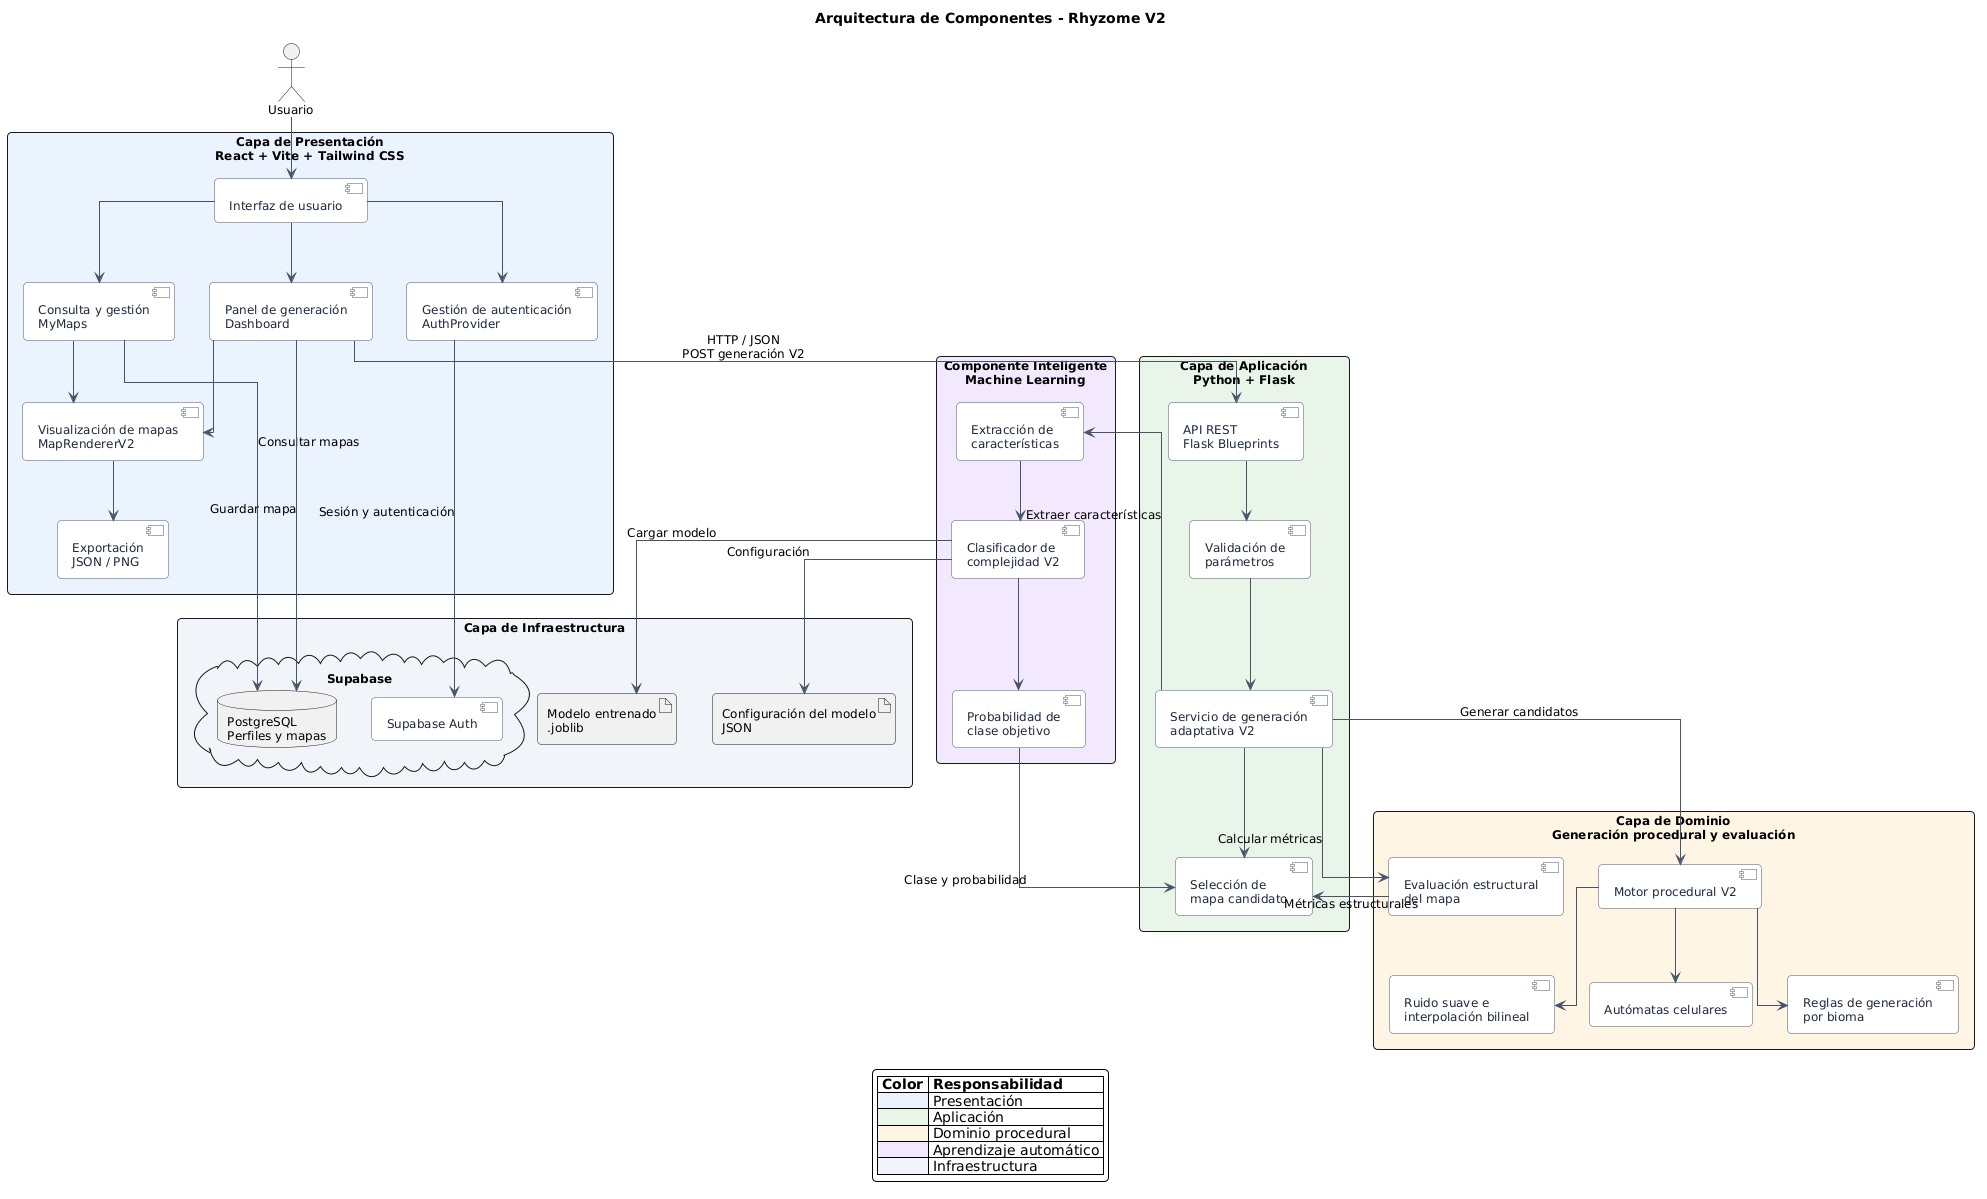
\includegraphics[width=\linewidth,height=0.78\vsize,keepaspectratio]{imagenes/ComponenteV2.png}
		\caption{Arquitectura de componentes de Rhyzome V2}
		\label{fig:arquitectura_componentes}
	\end{figure}
\end{landscape}

\FloatBarrier

La arquitectura se encuentra organizada en los siguientes bloques funcionales:

\begin{itemize}
	
	\item \textbf{Capa de presentación:}
	implementada mediante React, Vite y Tailwind CSS. Proporciona las funcionalidades de autenticación, configuración de parámetros, generación, visualización, consulta y exportación de mapas.
	
	\item \textbf{Capa de aplicación:}
	desarrollada mediante Python y Flask. Es responsable de exponer los servicios REST, validar los parámetros recibidos y coordinar el proceso de generación adaptativa.
	
	\item \textbf{Capa de dominio:}
	contiene los algoritmos de generación procedural, las reglas específicas de cada bioma y los mecanismos de evaluación estructural de los mapas. Su responsabilidad consiste en construir escenarios candidatos y determinar sus características.
	
	\item \textbf{Componente inteligente:}
	integra los mecanismos de extracción de características y clasificación mediante aprendizaje automático. El modelo estima la complejidad de los mapas candidatos y proporciona información para apoyar la selección del escenario final.
	
	\item \textbf{Capa de infraestructura:}
	proporciona los recursos necesarios para la autenticación, persistencia de información, almacenamiento de mapas y carga de los artefactos del modelo de aprendizaje automático.
	
\end{itemize}

La comunicación entre el frontend y el backend se realiza mediante servicios REST y estructuras de datos en formato JSON, permitiendo mantener independientes los componentes de presentación y procesamiento.

El modelo de aprendizaje automático clasifica los mapas candidatos; los algoritmos procedurales construyen los escenarios. El flujo de selección se desarrolla en la Sección~\ref{subsec:estrategia_generacion_adaptativa}.

\subsection{Flujo funcional del sistema (SBPMN)}
\label{subsec:flujo_funcional}

El flujo funcional de Rhyzome representa la secuencia de actividades que intervienen en la generación, evaluación y administración de mapas procedurales, identificando las responsabilidades del usuario, la interfaz web, los servicios de procesamiento y el componente inteligente.

La representación del proceso permite identificar los puntos de interacción, las decisiones asociadas a la generación procedural y los mecanismos de comunicación entre los componentes del sistema. La Figura~\ref{fig:flujo_funcional} presenta el flujo funcional correspondiente a la versión definitiva del prototipo Rhyzome.


\FloatBarrier
\clearpage

\begin{figure}[H]
	\centering
	
	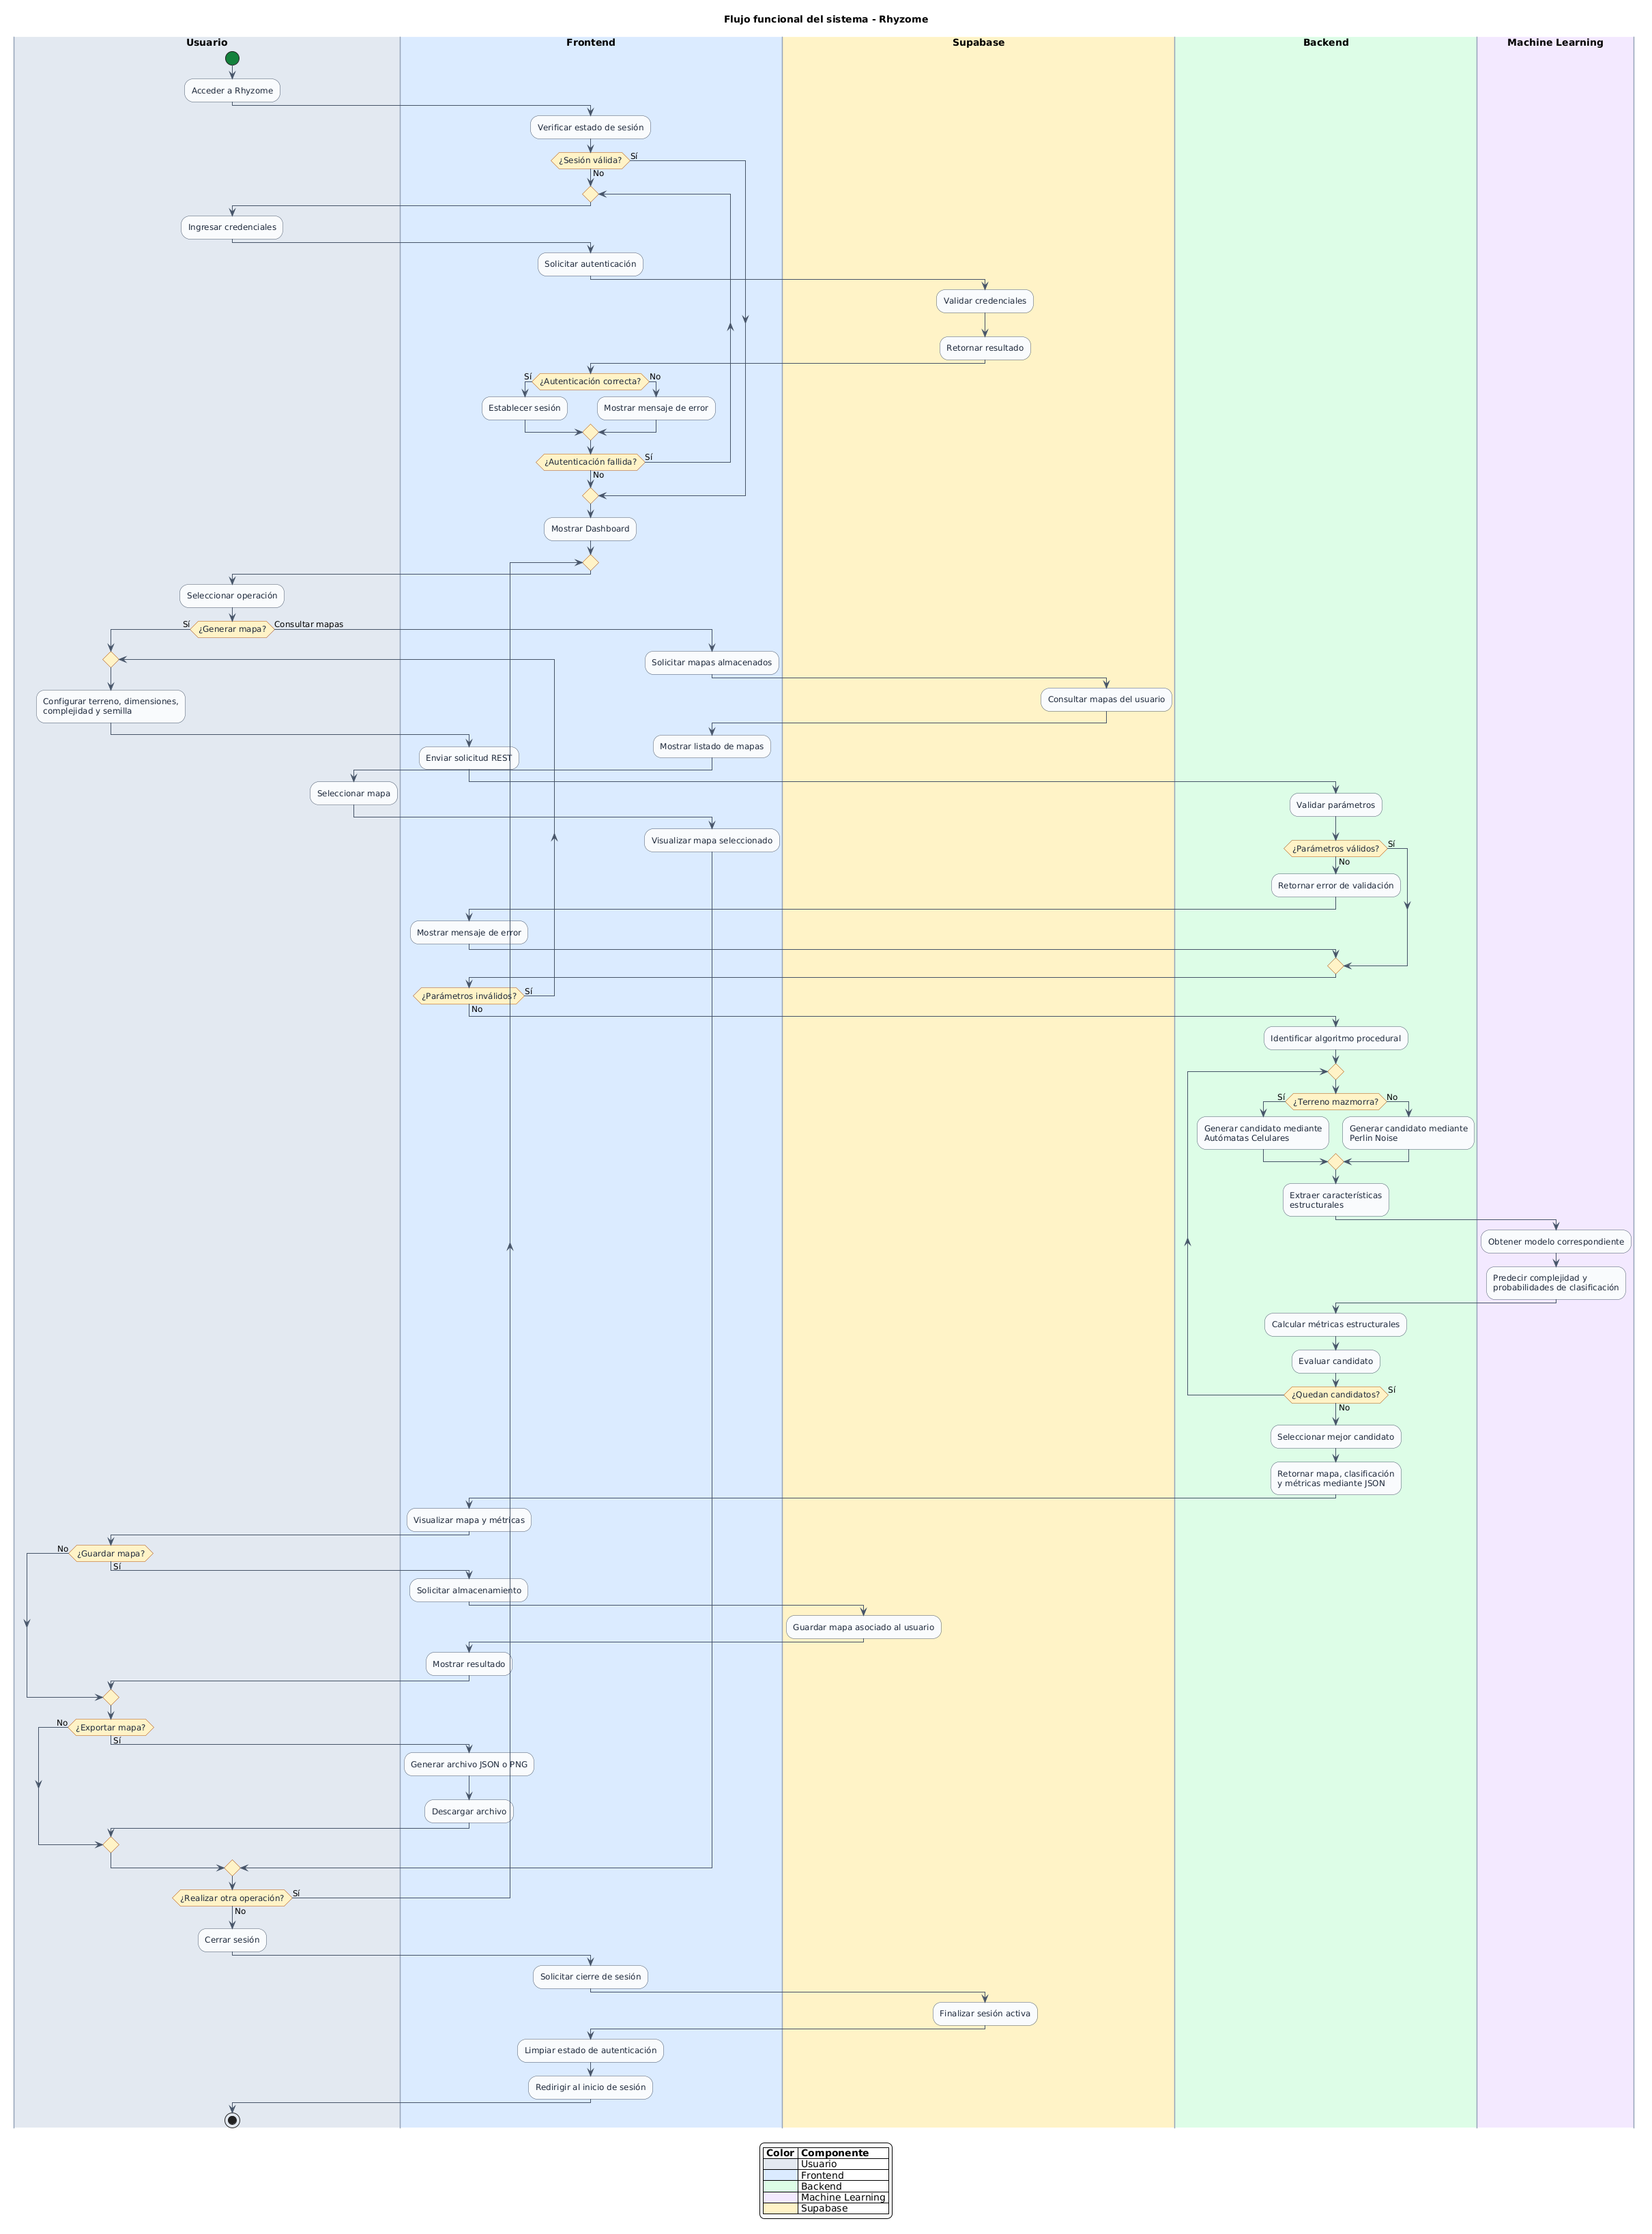
\includegraphics[
	width=\textwidth,
	height=0.90\textheight,
	keepaspectratio
	]{imagenes/flujo_funcional_rhyzome.png}
	
	\caption{Flujo funcional del sistema Rhyzome}
	\label{fig:flujo_funcional}
\end{figure}

\FloatBarrier
\clearpage


El proceso se organiza en cuatro etapas principales:

\begin{enumerate}
	
	\item \textbf{Acceso y configuración:}
	el usuario accede a la aplicación mediante una sesión válida y establece los parámetros necesarios para la generación del escenario.
	
	\item \textbf{Generación procedural:}
	el backend valida los parámetros recibidos y ejecuta el algoritmo correspondiente al tipo de terreno seleccionado, construyendo los mapas candidatos.
	
	\item \textbf{Evaluación y selección adaptativa:}
	se extraen las características estructurales de los candidatos y se utiliza el modelo de aprendizaje automático correspondiente para estimar su nivel de complejidad. Los resultados de clasificación y evaluación permiten seleccionar
	el escenario disponible que mejor se ajusta a los criterios establecidos.
	
	\item \textbf{Presentación y administración:}
	la interfaz visualiza el mapa seleccionado junto con sus métricas estructurales, proporcionando opciones de almacenamiento, consulta y exportación.
	
\end{enumerate}

El flujo contempla mecanismos de validación de parámetros y control de acceso, así como la separación entre las actividades de generación procedural y clasificación mediante aprendizaje automático.

Los detalles técnicos del mecanismo de generación adaptativa se desarrollan en la Sección~\ref{sec:integracion_ia}, mientras que la
evaluación experimental de los modelos y la validación funcional del sistema se presentan en los capítulos correspondientes.

\FloatBarrier

\section{Diagrama de despliegue}
\label{sec:diagrama_despliegue}

El despliegue de Rhyzome se fundamenta en una arquitectura distribuida que integra diferentes servicios en la nube para proporcionar las
funcionalidades de presentación, procesamiento, autenticación y persistencia de información.

Esta distribución permite mantener separados los componentes del frontend y backend, facilitando su administración, mantenimiento y actualización de manera independiente.

La Figura~\ref{fig:despliegue_rhyzome} presenta el diagrama de despliegue correspondiente a la versión V2 de Rhyzome, identificando los nodos de ejecución, los artefactos de software y los mecanismos de comunicación utilizados por el sistema.

\begin{landscape}
	\begin{figure}[H]
		\centering
		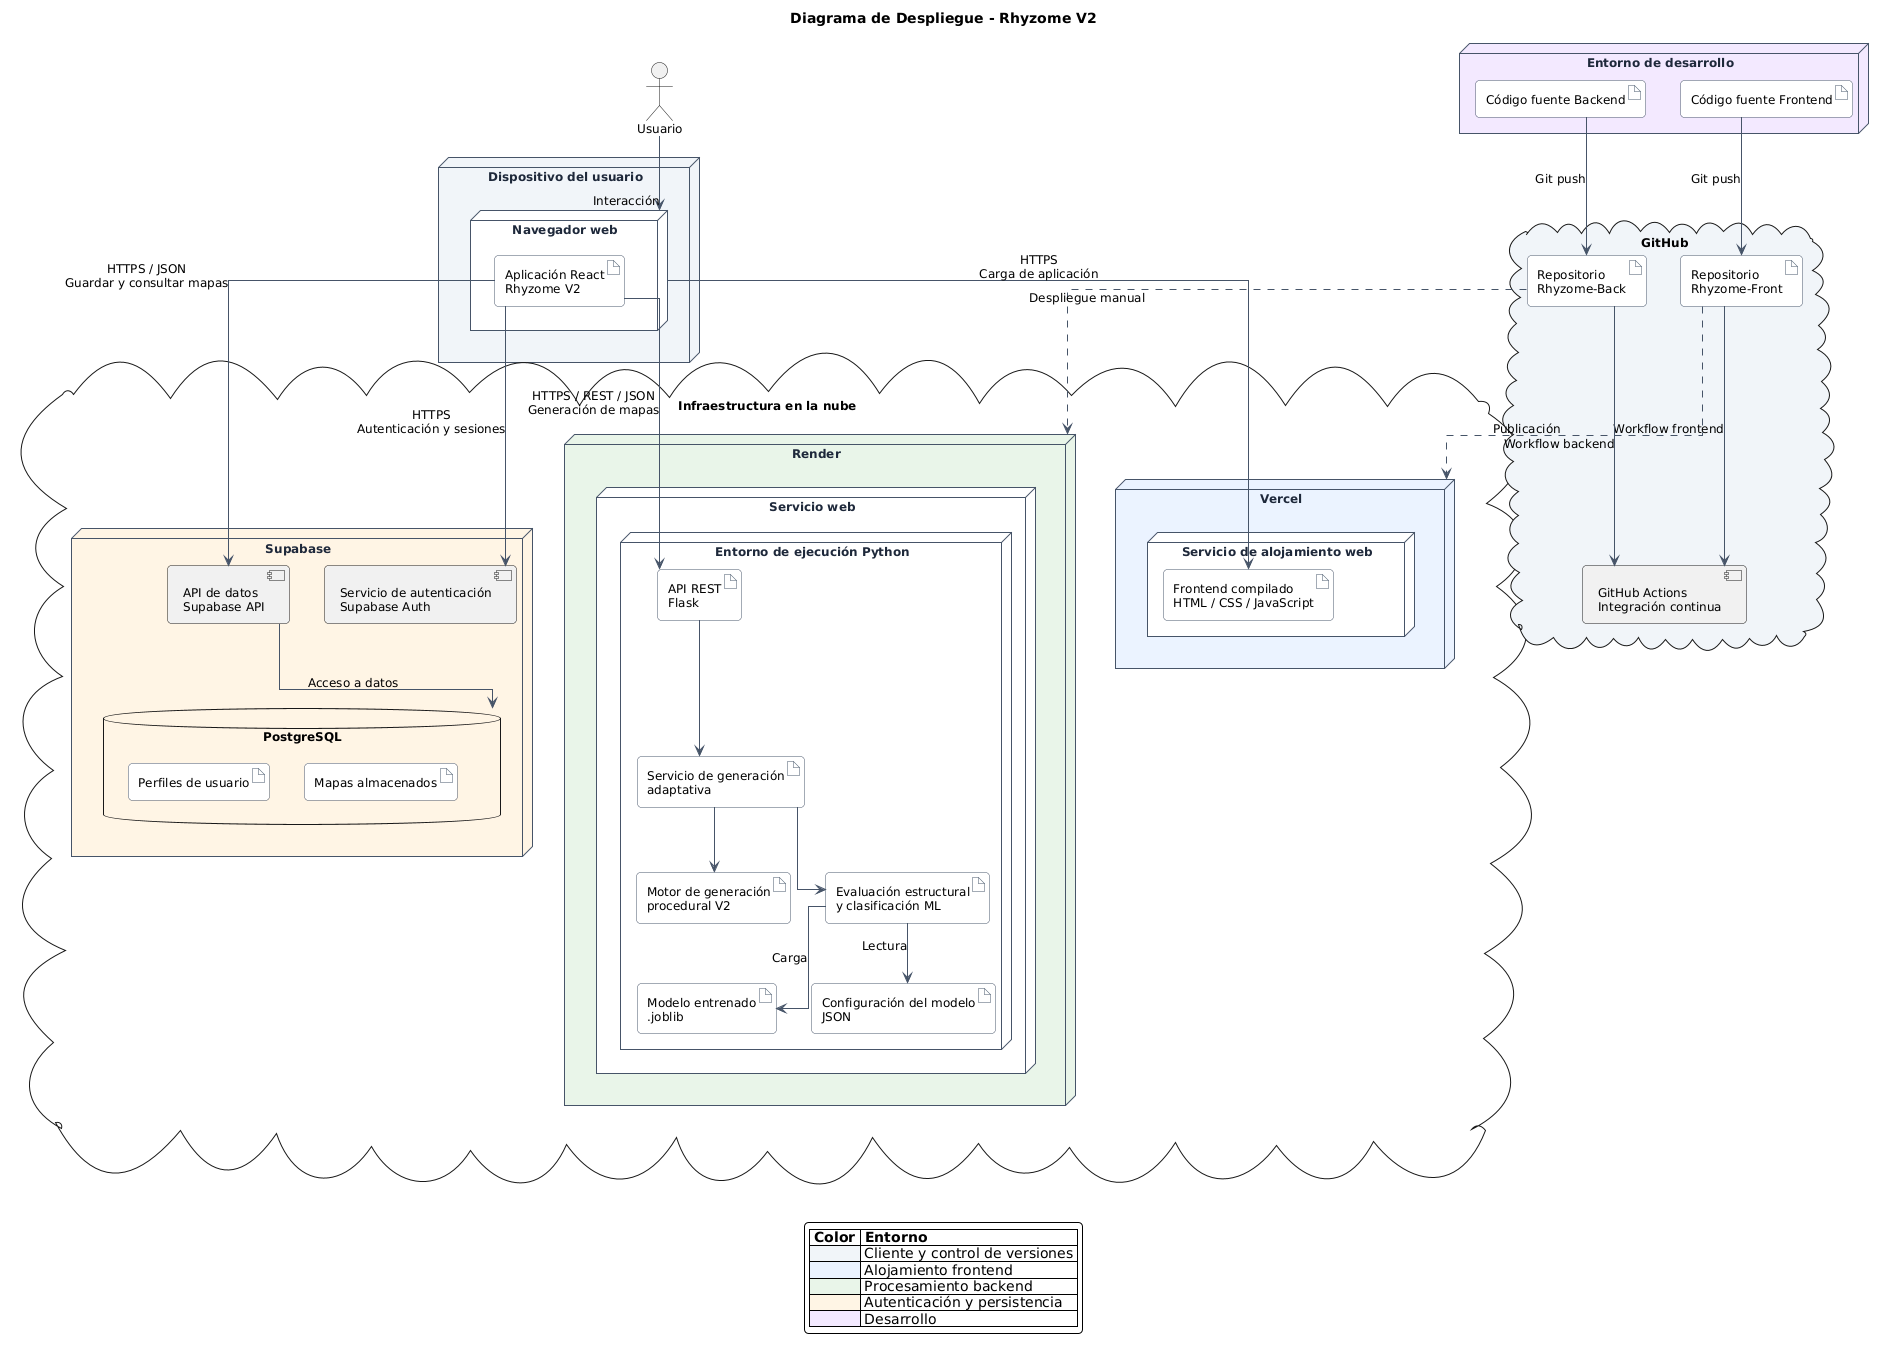
\includegraphics[width=\linewidth,height=0.78\vsize,keepaspectratio]{imagenes/despliegue.png}
		\caption{Diagrama de despliegue de Rhyzome V2}
		\label{fig:despliegue_rhyzome}
	\end{figure}
\end{landscape}

\FloatBarrier

\subsection{Distribución de la infraestructura}

La infraestructura tecnológica de Rhyzome se encuentra distribuida en los siguientes nodos y servicios:

\begin{itemize}
	
	\item \textbf{Dispositivo del usuario:}
	corresponde al equipo desde el cual se accede a la aplicación mediante un navegador web. En este entorno se ejecuta la aplicación desarrollada en React, proporcionando las funcionalidades de autenticación, configuración, generación, visualización y consulta de mapas.
	
	\item \textbf{Vercel:}
	plataforma utilizada para el alojamiento y distribución del frontend. Contiene los archivos compilados de la aplicación web,  permitiendo su acceso mediante el protocolo HTTPS desde diferentes dispositivos.
	
	\item \textbf{Render:}
	plataforma encargada del alojamiento del backend desarrollado en Python y Flask. En este entorno se ejecutan los servicios REST, los algoritmos de generación procedural, la evaluación estructural de los mapas y el componente de aprendizaje automático.
	
	\item \textbf{Supabase:}
	plataforma que proporciona los servicios de autenticación y persistencia de información. Integra una base de datos PostgreSQL utilizada
	para administrar los perfiles de usuario y los mapas almacenados por la aplicación.
	
	\item \textbf{GitHub:}
	plataforma utilizada para el control de versiones del código fuente del frontend y backend. Adicionalmente, mediante GitHub Actions se automatiza la ejecución de pruebas y otros procesos de integración continua.
	
	\item \textbf{Entorno de desarrollo:}
	corresponde al ambiente local en el cual se realizan las actividades de implementación, mantenimiento, pruebas y actualización del
	código fuente antes de su publicación en los ambientes correspondientes.
	
\end{itemize}

\subsection{Comunicación entre los componentes}

La comunicación entre los diferentes nodos del sistema se realiza mediante protocolos web y servicios REST.

Inicialmente, el navegador del usuario establece una conexión HTTPS con Vercel para obtener los archivos necesarios para la ejecución del frontend. Una vez cargada la aplicación, las solicitudes relacionadas con la generación procedural de mapas se envían directamente desde el navegador hacia los servicios REST desplegados en Render, mediante estructuras de datos en formato JSON. El backend procesa los parámetros recibidos, ejecuta los algoritmos de generación procedural, calcula las características estructurales de los mapas y utiliza el modelo de aprendizaje automático para apoyar la evaluación y selección de los escenarios generados. Por otra parte, las operaciones relacionadas con la autenticación, la administración de sesiones y la persistencia de mapas se realizan mediante los servicios proporcionados por Supabase.

Esta distribución permite que las operaciones de generación procedural y aprendizaje automático se ejecuten en el backend, evitando trasladar el procesamiento computacional al dispositivo del usuario.

\subsection{Estrategia de despliegue}

El proyecto utiliza repositorios independientes para la administración del código fuente del frontend y backend, permitiendo gestionar de
manera separada los cambios realizados sobre cada componente.

La integración continua se apoya en GitHub Actions, mediante flujos de trabajo destinados a la ejecución de pruebas automatizadas y
la verificación del código fuente.

La publicación del frontend se realiza mediante Vercel, mientras que el backend se encuentra alojado en Render. Para la versión actual del
prototipo, el despliegue del backend requiere la activación manual del proceso de publicación.

La separación entre los ambientes de desarrollo y producción facilita la validación de los cambios antes de su incorporación a la versión disponible para los usuarios.

\subsection{Consideraciones de infraestructura}

La arquitectura de despliegue seleccionada proporciona una base para la evolución independiente de los componentes del sistema, permitiendo realizar actualizaciones sobre la interfaz, los servicios REST y los modelos de aprendizaje automático. Sin embargo, el rendimiento del sistema depende de los recursos computacionales disponibles en las plataformas de alojamiento, especialmente durante la ejecución de los procesos de generación adaptativa.

En particular, los tiempos de respuesta pueden verse afectados por la inicialización del servicio backend, las dimensiones de los mapas solicitados y la cantidad de candidatos generados durante cada solicitud. Estos factores son relevantes para la evaluación del rendimiento y la identificación de futuras oportunidades de optimización del prototipo.

La evaluación de los tiempos de respuesta y los resultados de las pruebas realizadas se presentan posteriormente en el capítulo de pruebas y validación.

\begin{table}[htbp]
	\centering
	
	\caption{Distribución de los servicios de Rhyzome}
	\label{tab:infraestructura_despliegue}
	
	\renewcommand{\arraystretch}{1.5}
	
	\begin{tabularx}{\textwidth}{
			|>{\raggedright\arraybackslash}p{3cm}|
			>{\raggedright\arraybackslash}p{3cm}|
			>{\raggedright\arraybackslash}X|
		}
		\hline
		
		\rowcolor{gray!15}
		\textbf{Plataforma} &
		\textbf{Componente} &
		\textbf{Responsabilidad} \\
		
		\hline
		
		\textbf{Vercel} &
		Frontend &
		Alojamiento y distribución de la aplicación web desarrollada mediante React, Vite y Tailwind CSS. \\
		
		\hline
		
		\textbf{Render} &
		Backend &
		Ejecución de los servicios REST, algoritmos de generación procedural, evaluación estructural e inferencia de los
		modelos de aprendizaje automático. \\
		
		\hline
		
		\textbf{Supabase} &
		Autenticación &
		Gestión de usuarios, sesiones, inicio de sesión y recuperación de contraseñas. \\
		
		\hline
		
		\textbf{Supabase} &
		PostgreSQL &
		Persistencia y consulta de perfiles de usuario y mapas almacenados en la aplicación. \\
		
		\hline
		
		\textbf{GitHub} &
		Repositorios &
		Control de versiones, administración y trazabilidad de los cambios realizados en el código fuente del frontend y backend. \\
		
		\hline
		
		\textbf{GitHub Actions} &
		Integración continua &
		Ejecución automatizada de pruebas, generación de reportes de cobertura y verificación del código fuente. \\
		
		\hline
		
	\end{tabularx}
	
	\par\smallskip
	\raggedright
	
	\textit{Nota.} La distribución presentada corresponde a la infraestructura tecnológica utilizada en Rhyzome V2. La separación de los servicios permite administrar de manera independiente los componentes de presentación, procesamiento, autenticación y persistencia de información.
	
\end{table}

\FloatBarrier

\section{Tecnologías y frameworks utilizados}
\label{sec:tecnologias_frameworks}

El desarrollo de Rhyzome se fundamenta en la integración de tecnologías orientadas al desarrollo web, la generación procedural de contenido, el aprendizaje automático y la administración de servicios en la nube.

La selección de estas tecnologías se realizó considerando criterios de compatibilidad, modularidad, facilidad de integración, mantenimiento y disponibilidad de herramientas para el desarrollo del prototipo.

La arquitectura tecnológica permite separar las responsabilidades de presentación, procesamiento, persistencia de información e inferencia de los modelos de aprendizaje automático.

\subsection{Stack tecnológico}

La Tabla~\ref{tab:stack_tecnologico} presenta las principales tecnologías y frameworks utilizados en la implementación de Rhyzome, identificando su categoría y responsabilidad dentro del sistema.

\begin{table}[htbp]
	\centering
	
	\caption{Tecnologías y frameworks utilizados en Rhyzome}
	\label{tab:stack_tecnologico}
	
	\renewcommand{\arraystretch}{1.5}
	
	\begin{tabularx}{\textwidth}{
			|>{\raggedright\arraybackslash}p{2.8cm}|
			>{\raggedright\arraybackslash}p{2.8cm}|
			>{\raggedright\arraybackslash}X|
		}
		\hline
		
		\rowcolor{gray!15}
		\textbf{Tecnología} &
		\textbf{Categoría} &
		\textbf{Responsabilidad} \\
		
		\hline
		
		\textbf{Python} &
		Lenguaje de programación &
		Implementación del backend, los algoritmos de generación procedural y el componente de aprendizaje automático. \\
		
		\hline
		
		\textbf{JavaScript} &
		Lenguaje de programación &
		Implementación de la lógica de interacción y comportamiento de la aplicación web. \\
		
		\hline
		
		\textbf{Flask} &
		Framework backend &
		Implementación de los servicios REST y coordinación de las solicitudes de generación de mapas. \\
		
		\hline
		
		\textbf{React} &
		Biblioteca frontend &
		Construcción de interfaces mediante componentes reutilizables y gestión del estado de la aplicación. \\
		
		\hline
		
		\textbf{Vite} &
		Herramienta de construcción &
		Configuración del entorno de desarrollo y compilación de la aplicación frontend. \\
		
		\hline
		
		\textbf{Tailwind CSS} &
		Framework CSS &
		Definición de estilos, distribución visual y diseño adaptable de la interfaz de usuario. \\
		
		\hline
		
		\textbf{React Router} &
		Enrutamiento &
		Administración de la navegación y protección de rutas privadas en la aplicación. \\
		
		\hline
		
		\textbf{NumPy} &
		Computación científica &
		Procesamiento de matrices, operaciones numéricas y representación de estructuras de mapas. \\
		
		\hline
		
		\textbf{SciPy} &
		Computación científica &
		Apoyo al procesamiento numérico y análisis de características estructurales. \\
		
		\hline
		
		\textbf{Scikit-learn} &
		Aprendizaje automático &
		Implementación y utilización de modelos supervisados para la clasificación de complejidad de los mapas. \\
		
		\hline
		
		\textbf{Joblib} &
		Serialización &
		Almacenamiento y carga de los artefactos de los modelos de aprendizaje automático. \\
		
		\hline
		
		\textbf{Supabase} &
		Backend como servicio &
		Administración de la autenticación, sesiones y persistencia de información. \\
		
		\hline
		
		\textbf{PostgreSQL} &
		Base de datos relacional &
		Almacenamiento de perfiles de usuario y mapas registrados en la aplicación. \\
		
		\hline
		
	\end{tabularx}
	
	\par\smallskip
	\raggedright
	
	\textit{Nota.} Las tecnologías presentadas corresponden al stack tecnológico de Rhyzome y se encuentran agrupadas de acuerdo con su responsabilidad dentro de la arquitectura del sistema.
	
\end{table}

\FloatBarrier

\subsection{Herramientas de desarrollo y soporte}

Además de las tecnologías utilizadas en la implementación del sistema, el proyecto incorpora herramientas de soporte orientadas al control de versiones, la automatización de pruebas, el despliegue y la gestión del desarrollo.

La Tabla~\ref{tab:herramientas_soporte} presenta las herramientas que respaldan estas actividades.

\begin{table}[htbp]
	\centering
	
	\caption{Herramientas de desarrollo y soporte de Rhyzome}
	\label{tab:herramientas_soporte}
	
	\renewcommand{\arraystretch}{1.5}
	
	\begin{tabularx}{\textwidth}{
			|>{\raggedright\arraybackslash}p{2.8cm}|
			>{\raggedright\arraybackslash}p{2.8cm}|
			>{\raggedright\arraybackslash}X|
		}
		\hline
		
		\rowcolor{gray!15}
		\textbf{Herramienta} &
		\textbf{Categoría} &
		\textbf{Responsabilidad} \\
		
		\hline
		
		\textbf{Git} &
		Control de versiones &
		Administración del historial de cambios del código fuente. \\
		
		\hline
		
		\textbf{GitHub} &
		Repositorios &
		Almacenamiento y administración de los repositorios del frontend y backend. \\
		
		\hline
		
		\textbf{GitHub Actions} &
		Integración continua &
		Automatización de pruebas y generación de reportes de ejecución y cobertura. \\
		
		\hline
		
		\textbf{Pytest} &
		Pruebas backend &
		Ejecución de pruebas unitarias, funcionales y de integración sobre los componentes desarrollados en Python. \\
		
		\hline
		
		\textbf{Vitest} &
		Pruebas frontend &
		Validación automatizada de componentes y servicios de la aplicación web. \\
		
		\hline
		
		\textbf{Postman} &
		Validación de API &
		Ejecución manual de solicitudes HTTP y verificación de los contratos de comunicación REST. \\
		
		\hline
		
		\textbf{Vercel} &
		Despliegue &
		Alojamiento y distribución del frontend. \\
		
		\hline
		
		\textbf{Render} &
		Despliegue &
		Alojamiento y ejecución de los servicios backend. \\
		
		\hline
		
		\textbf{Jira} &
		Gestión ágil &
		Administración del Product Backlog, historias de usuario, sprints y seguimiento del proyecto. \\
		
		\hline
		
		\textbf{Confluence} &
		Documentación &
		Organización de la documentación técnica y evidencias del proyecto. \\
		
		\hline
		
	\end{tabularx}
	
	\par\smallskip
	\raggedright
	
	\textit{Nota.} Las herramientas de soporte contribuyen a la trazabilidad, verificación, documentación y mantenimiento del proyecto durante su ciclo de desarrollo.
	
\end{table}

\FloatBarrier

\subsection{Justificación de la selección tecnológica}

La selección de las tecnologías utilizadas en Rhyzome responde a las necesidades funcionales y técnicas identificadas durante el diseño de la solución.

\subsubsection{Tecnologías de frontend}

React fue seleccionado por su enfoque basado en componentes reutilizables, el cual facilita la construcción de interfaces modulares y la separación de responsabilidades visuales.

Su integración con Vite y Tailwind CSS permite disponer de un entorno de desarrollo orientado a la construcción de interfaces web interactivas y al mantenimiento de una estructura visual consistente.

\subsubsection{Tecnologías de backend}

Python fue seleccionado debido a su ecosistema de bibliotecas orientadas al procesamiento numérico, la generación procedural y el aprendizaje automático.

Flask proporciona una estructura flexible para la implementación de servicios REST, permitiendo organizar las funcionalidades del backend mediante módulos y mantener separada la lógica de procesamiento de la interfaz de usuario.

\subsubsection{Generación procedural y aprendizaje automático}

NumPy y SciPy proporcionan herramientas para el procesamiento de matrices y el análisis numérico de las estructuras generadas por los algoritmos procedurales.

Scikit-learn permite integrar modelos de clasificación supervisada dentro del proceso de generación adaptativa, mientras que Joblib facilita la serialización y carga de los modelos entrenados.

La utilización de estas tecnologías permite integrar la generación procedural y la inferencia de aprendizaje automático dentro de un mismo entorno de ejecución.

\subsubsection{Autenticación y persistencia}

Supabase fue seleccionado como servicio externo para la administración de usuarios, sesiones y persistencia de información.

La integración con PostgreSQL permite gestionar los datos asociados a los usuarios y los mapas almacenados, reduciendo la necesidad de implementar desde cero un servicio independiente de administración de datos.

\subsubsection{Despliegue y aseguramiento de la calidad}

La utilización de Vercel y Render permite mantener separados los ambientes de alojamiento del frontend y backend.

GitHub Actions, Pytest y Vitest complementan esta arquitectura mediante mecanismos de integración continua y validación automatizada, contribuyendo a la detección de errores y al mantenimiento del código fuente.

En conjunto, las tecnologías seleccionadas proporcionan una base modular para el desarrollo del prototipo, facilitando la integración de sus componentes y permitiendo su evolución de acuerdo con las necesidades identificadas durante el proyecto.

\section{Diseño de la interfaz de usuario}
\label{sec:diseno_interfaz_usuario}

El diseño de la interfaz de usuario de Rhyzome se orienta a proporcionar un entorno interactivo que facilite la configuración, generación, visualización, evaluación y administración de mapas procedurales para videojuegos 2D.

La interfaz permite que los usuarios interactúen con los algoritmos de generación procedural y el componente de aprendizaje automático sin necesidad de conocer los detalles internos de su implementación.

Su desarrollo se realizó mediante React, Vite y Tailwind CSS, utilizando una estructura basada en componentes reutilizables que permite separar las responsabilidades visuales y funcionales de la aplicación.

\subsection{Metodología de diseño}

El diseño de la interfaz se desarrolló mediante un proceso incremental e iterativo, articulado con la metodología ágil adoptada en el proyecto. Inicialmente, se identificaron las necesidades funcionales de los usuarios relacionadas con la configuración de parámetros, la generación procedural, la visualización y la administración de mapas. A partir de estas necesidades, se definió la organización de la información y la distribución de las funcionalidades principales dentro de la aplicación.

El proceso de diseño contempló las siguientes actividades:

\begin{enumerate}
	
	\item Identificación de las necesidades y funcionalidades requeridas por los usuarios.
	
	\item Definición de la arquitectura de información y los mecanismos de navegación.
	
	\item Construcción de una interfaz inicial para la configuración y visualización de mapas.
	
	\item Integración de los servicios de generación procedural y aprendizaje automático.
	
	\item Mejoramiento progresivo de los componentes visuales y mecanismos de interacción.
	
	\item Incorporación de funcionalidades de autenticación, almacenamiento, consulta y exportación de mapas.
	
	\item Validación funcional de las interfaces implementadas.
	
\end{enumerate}

La evolución de la interfaz permitió incorporar nuevas funcionalidades de manera progresiva, manteniendo la coherencia con los requerimientos del proyecto y las historias de usuario definidas durante las iteraciones de desarrollo.

\subsection{Arquitectura de información y navegación}

La arquitectura de información de Rhyzome organiza las funcionalidades del sistema mediante una separación entre interfaces públicas, interfaces privadas y operaciones asociadas a la generación procedural de mapas.

Las interfaces públicas permiten realizar operaciones de autenticación, registro y recuperación de contraseña, mientras que las interfaces privadas proporcionan acceso a las funcionalidades principales del generador.

La Figura~\ref{fig:navegacion_interfaz} representa la organización funcional de las interfaces y las relaciones de navegación existentes entre ellas.

\begin{figure}[H]
	\centering
	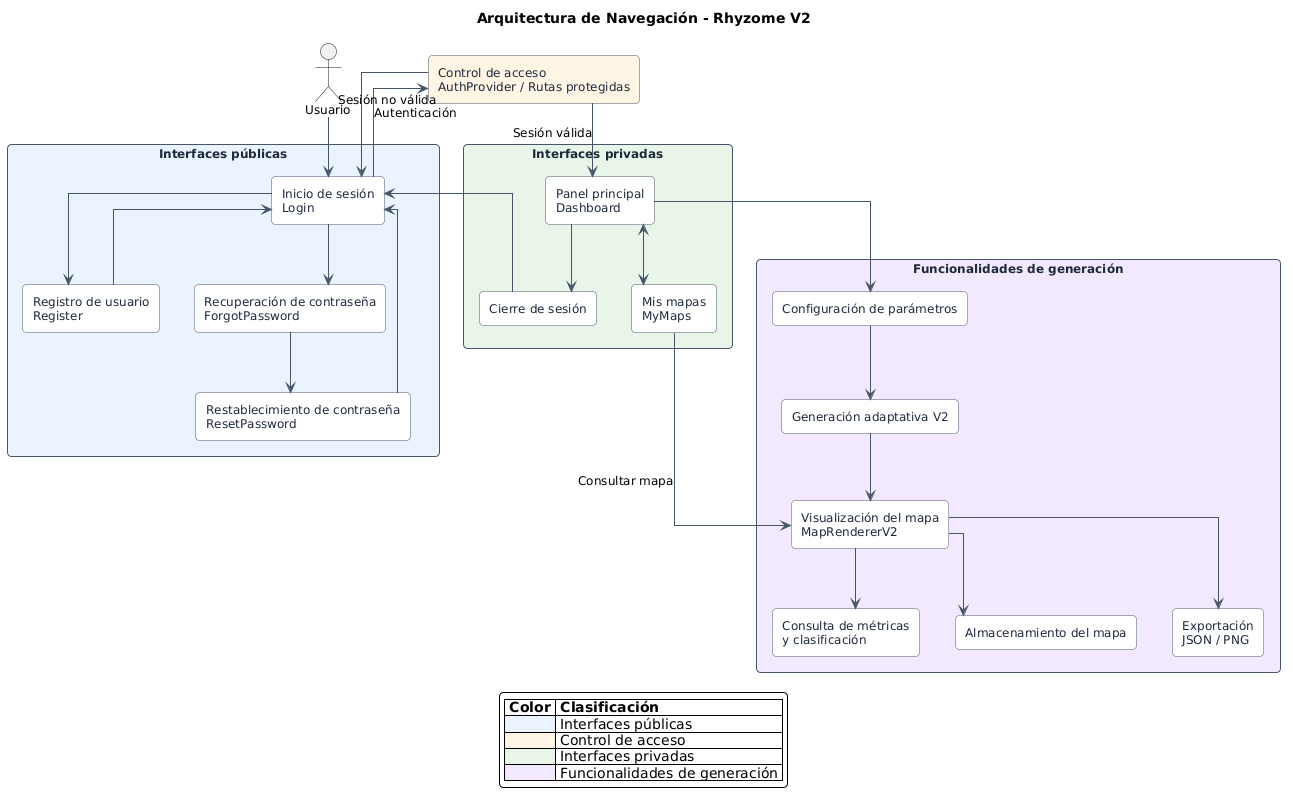
\includegraphics[width=\textwidth]{imagenes/navegacion.png}
	\caption{Arquitectura de navegación de Rhyzome V2}
	\label{fig:navegacion_interfaz}
\end{figure}

\FloatBarrier

Como se observa en la figura, el acceso a las funcionalidades principales se encuentra condicionado por la existencia de una sesión válida.

Una vez autenticado, el usuario puede acceder al panel principal de generación y consultar los mapas almacenados.

Esta organización permite diferenciar las operaciones relacionadas con la administración de usuarios de aquellas orientadas a la generación, visualización y gestión de mapas procedurales.

\subsection{Criterios y decisiones de diseño}

El diseño de la interfaz de Rhyzome consideró criterios orientados a facilitar la interacción, mantener la consistencia visual y organizar las funcionalidades de acuerdo con las tareas realizadas por el usuario.

La Tabla~\ref{tab:criterios_diseno_interfaz} presenta los principales criterios considerados durante el desarrollo de la interfaz.

\begin{table}[htbp]
	\centering
	
	\caption{Criterios de diseño de la interfaz de Rhyzome}
	\label{tab:criterios_diseno_interfaz}
	
	\renewcommand{\arraystretch}{1.5}
	
	\begin{tabularx}{\textwidth}{
			|>{\raggedright\arraybackslash}p{3.5cm}|
			>{\raggedright\arraybackslash}X|
		}
		\hline
		
		\rowcolor{gray!15}
		\textbf{Criterio} &
		\textbf{Aplicación en Rhyzome} \\
		
		\hline
		
		\textbf{Consistencia visual} &
		Utilización de estilos, colores y componentes reutilizables para mantener una presentación uniforme entre las interfaces. \\
		
		\hline
		
		\textbf{Jerarquía visual} &
		Organización de los controles y resultados de acuerdo con su importancia dentro del proceso de generación procedural. \\
		
		\hline
		
		\textbf{Facilidad de interacción} &
		Agrupación de los parámetros y acciones principales dentro del panel de generación. \\
		
		\hline
		
		\textbf{Retroalimentación} &
		Presentación de información relacionada con el procesamiento de solicitudes, resultados y errores de la aplicación. \\
		
		\hline
		
		\textbf{Diferenciación de terrenos} &
		Representación visual de los escenarios mediante colores y elementos asociados a las características del terreno generado. \\
		
		\hline
		
		\textbf{Control de acceso} &
		Separación de las interfaces públicas y privadas, condicionando el acceso a una sesión válida. \\
		
		\hline
		
		\textbf{Modularidad} &
		Implementación de componentes React reutilizables para facilitar el mantenimiento y evolución de la interfaz. \\
		
		\hline
		
		\textbf{Control del usuario} &
		Disponibilidad de opciones para configurar, generar, consultar, almacenar y exportar mapas. \\
		
		\hline
		
	\end{tabularx}
	
	\par\smallskip
	\raggedright
	
	\textit{Nota.} Los criterios descritos corresponden a decisiones de diseño aplicadas durante el desarrollo incremental de la interfaz de Rhyzome.
	
\end{table}

\FloatBarrier

La aplicación de estos criterios busca reducir la complejidad de interacción con los algoritmos de generación procedural y el componente inteligente.

Asimismo, la separación de las funcionalidades permite organizar la experiencia de usuario alrededor de las principales tareas del sistema, evitando que los detalles técnicos de implementación interfieran directamente con el proceso de generación de mapas.

\subsection{Interfaz definitiva del prototipo}
\label{subsec:resultados_diseno_interfaz}

La interfaz de usuario de Rhyzome integra las funcionalidades de configuración, generación procedural, visualización, evaluación, almacenamiento y exportación de mapas dentro de un entorno web unificado.

El diseño presenta una organización funcional orientada a facilitar la interacción con los algoritmos de generación
procedural y el componente de aprendizaje automático, permitiendo configurar las características de los escenarios
sin requerir conocimientos sobre su implementación interna.

La representación gráfica de los mapas utiliza elementos visuales asociados a los diferentes tipos de terreno, permitiendo identificar las características y estructuras que conforman cada escenario generado.

La Figura~\ref{fig:resultado_final_interfaz} presenta la interfaz correspondiente a la versión definitiva del prototipo Rhyzome.

\begin{figure}[H]
	\centering
	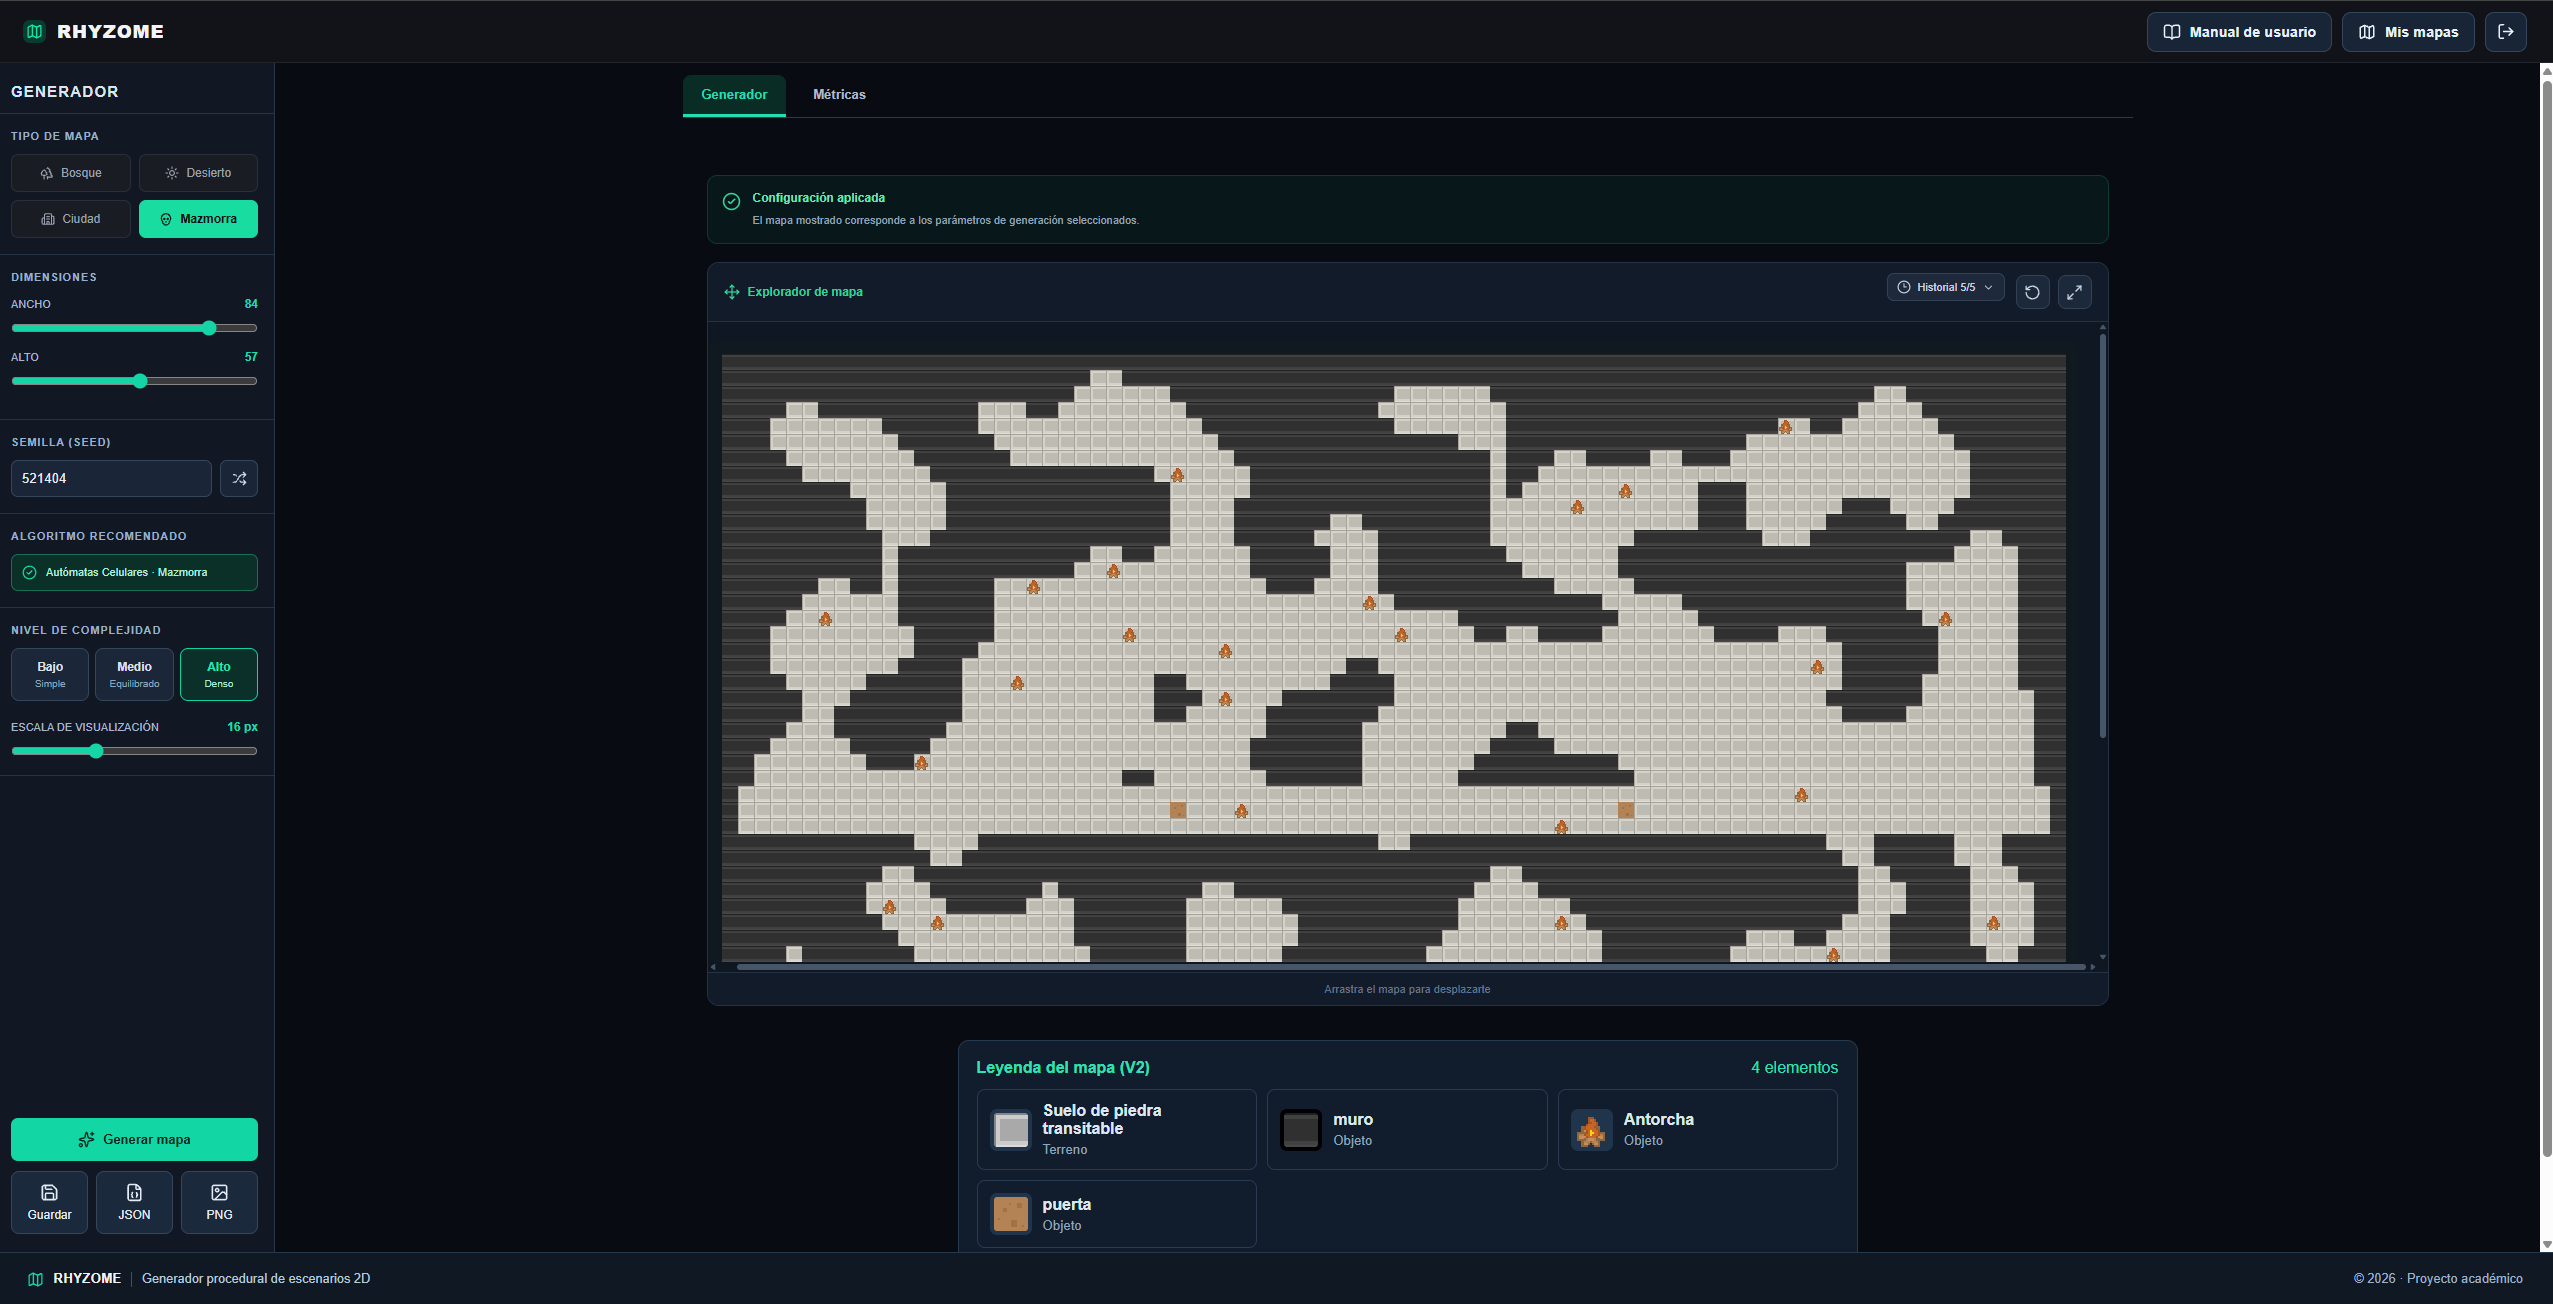
\includegraphics[width=\textwidth]{imagenes/mazmorra.png}
	\caption{Interfaz definitiva del prototipo Rhyzome}
	\label{fig:resultado_final_interfaz}
\end{figure}

El dashboard reúne los controles de terreno, dimensiones, complejidad y semilla, el área de visualización del mapa y las opciones de consulta de métricas, almacenamiento y exportación JSON y PNG. Los criterios de diseño se recogen en la Tabla~\ref{tab:criterios_diseno_interfaz}; la comprobación funcional corresponde al Capítulo~\ref{cap:06_pruebas_validacion}.

\FloatBarrier

\section{Estrategia de integración del modelo de IA}
\label{sec:integracion_ia}

\subsection{Flujo de generación adaptativa}
\label{subsec:estrategia_generacion_adaptativa}

La generación adaptativa integra la construcción procedural de mapas con la clasificación de complejidad mediante aprendizaje automático. El servicio de generación coordina la evaluación de los candidatos y selecciona el escenario que mejor se ajusta a la solicitud del usuario.

La Figura~\ref{fig:integracion_modelo_ia} presenta el diagrama de secuencia de este proceso. A diferencia del flujo funcional de la Figura~\ref{fig:flujo_funcional}, esta representación describe los intercambios entre los componentes de software durante una solicitud de generación.

\FloatBarrier

\begin{landscape}
	\begin{figure}[H]
		\centering
		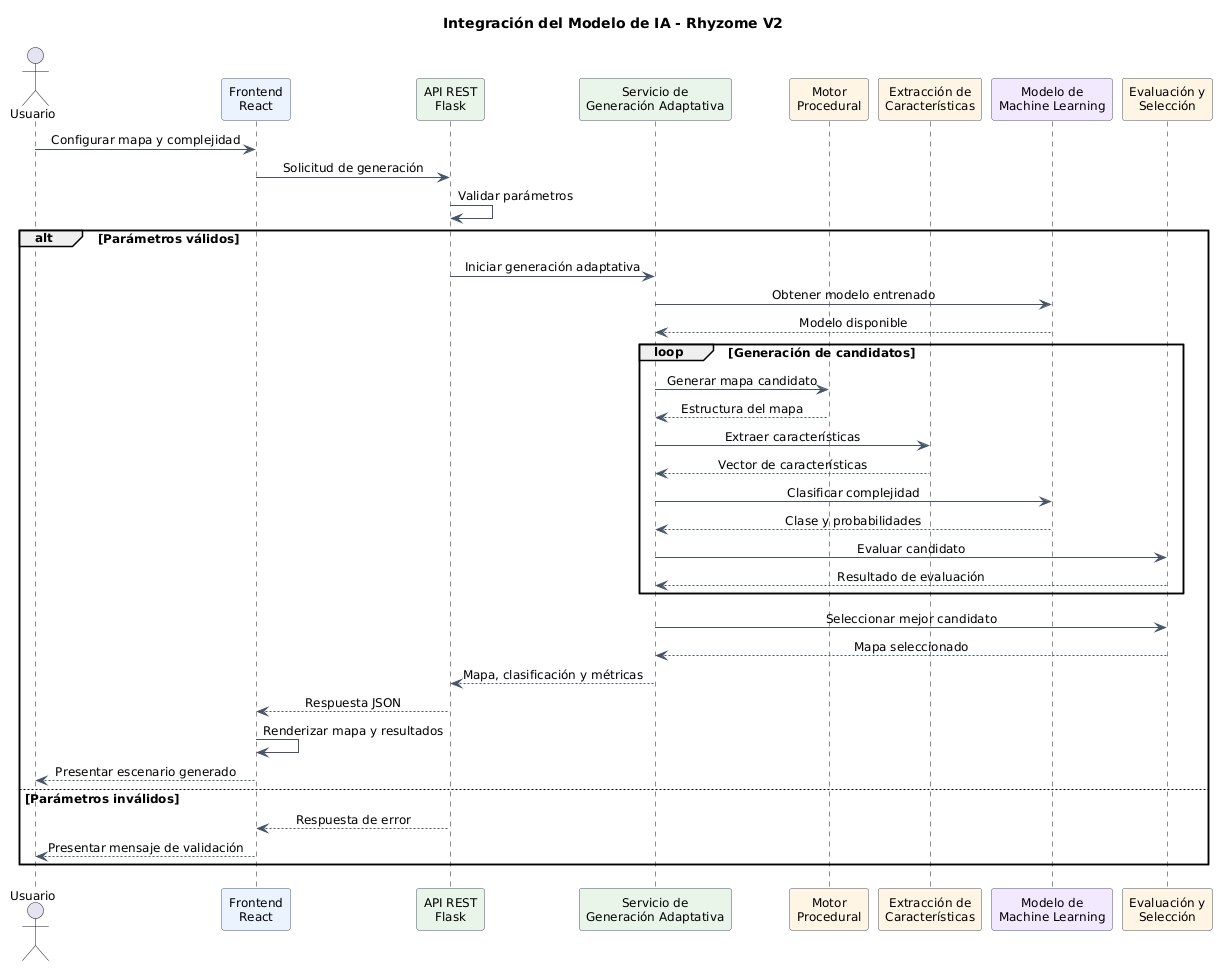
\includegraphics[
		width=\linewidth,
		height=0.78\vsize,
		keepaspectratio
		]{imagenes/integracion_modelo_ia.png}
		\caption{Diagrama de secuencia de integración del modelo de IA en Rhyzome}
		\label{fig:integracion_modelo_ia}
	\end{figure}
\end{landscape}

\FloatBarrier

La API REST recibe y valida los parámetros de generación. El servicio adaptativo coordina la construcción de los mapas candidatos mediante el algoritmo procedural correspondiente al terreno seleccionado. Para cada candidato se extraen sus características, se estima su complejidad mediante el clasificador correspondiente y se realiza la evaluación estructural. La selección considera los resultados obtenidos dentro del límite de intentos configurado. La respuesta se entrega en formato JSON e incluye el mapa seleccionado, su clasificación y sus métricas estructurales.

\subsubsection{Formalización del mecanismo de selección}
\label{subsubsec:formalizacion_seleccion}

El mecanismo de selección es el componente de la generación adaptativa encargado de comparar los mapas candidatos producidos por los algoritmos procedurales, con el propósito de identificar el escenario que mejor se ajusta al nivel de complejidad solicitado por el usuario. Para ello, integra los resultados de la clasificación mediante aprendizaje automático y la evaluación de las características estructurales de cada mapa. La siguiente formalización matemática describe los elementos que intervienen en este proceso, la estimación de la probabilidad de pertenencia a la clase objetivo y la representación conceptual del criterio utilizado para seleccionar el mapa resultante.

Sea $\mathcal{M}$ el conjunto de mapas candidatos obtenidos durante una solicitud de generación:

\begin{equation}
	\mathcal{M} = \{M_1,M_2,\ldots,M_n\}
	\label{eq:conjunto_candidatos}
\end{equation}

En esta expresión, $n$ representa la cantidad de candidatos considerados durante el proceso de generación adaptativa. Para cada mapa candidato se obtiene su representación numérica, su clasificación de complejidad y los resultados de evaluación estructural. A partir de su vector de características, el modelo de aprendizaje automático proporciona una estimación de la probabilidad de pertenencia a la clase de complejidad solicitada por el usuario, expresada mediante:

\begin{equation}
	p_i = P_{\theta}(y=c^{*}\mid\mathbf{x}_i)
	\label{eq:probabilidad_clase_objetivo}
\end{equation}

Los términos de la expresión se definen de la siguiente manera:

\begin{itemize}
	
	\item $c^{*}$ representa la clase de complejidad solicitada por el usuario.
	
	\item $\mathbf{x}_i$ corresponde al vector de características del mapa candidato $M_i$.
	
	\item $p_i$ representa la probabilidad estimada de pertenencia a la clase objetivo.
	
	\item $\theta$ representa los parámetros del modelo de aprendizaje automático entrenado.
	
	\item $y$ representa la variable asociada a la clase de complejidad.
	
\end{itemize}

La estrategia de selección utiliza la coincidencia entre la clase predicha y la clase objetivo, las probabilidades proporcionadas por el modelo y los resultados de evaluación estructural. Estos elementos permiten establecer criterios de preferencia entre los diferentes escenarios candidatos. Como representación conceptual, la selección del mapa resultante puede expresarse mediante:

\begin{equation}
	M^{*} =
	\underset{M_i \in \mathcal{M}}{\operatorname{arg\,max}}
	\; S(M_i,c^{*})
	\label{eq:seleccion_mapa}
\end{equation}

En esta expresión, $S$ representa el criterio de selección utilizado para comparar los escenarios candidatos y $M^{*}$ corresponde al mapa seleccionado. Esta expresión constituye una abstracción del mecanismo de selección y no implica necesariamente la utilización de una suma ponderada de métricas.

Cuando los candidatos no coinciden exactamente con la complejidad solicitada, el mecanismo de selección identifica el escenario disponible que presenta las condiciones más favorables de acuerdo con los criterios establecidos. Por consiguiente, la generación adaptativa se orienta a mejorar la correspondencia entre las características solicitadas y el escenario obtenido, sin garantizar una coincidencia absoluta en todas las solicitudes.

\subsection{Gestión de los modelos en producción}
\label{subsec:gestion_modelos_produccion}
El entrenamiento de los modelos de aprendizaje automático se realiza fuera del entorno de producción, separando la experimentación de la inferencia ejecutada por la aplicación. El backend carga artefactos serializados mediante Joblib y ejecuta la inferencia con scikit-learn \parencite{pedregosa2011}. La Tabla~\ref{tab:gestion_modelos_ia} identifica los artefactos, módulos y servicios documentados para la integración del componente inteligente.

\begin{table}[htbp]
	\centering
	
	\caption{Elementos técnicos de integración del modelo de IA}
	\label{tab:gestion_modelos_ia}
	
	\renewcommand{\arraystretch}{1.5}
	
	\begin{tabularx}{\textwidth}{
			|>{\raggedright\arraybackslash}p{5.5cm}|
			>{\raggedright\arraybackslash}X|
		}
		\hline
		
		\rowcolor{gray!15}
		\textbf{Elemento} &
		\textbf{Responsabilidad o justificación} \\
		\hline
		
		\texttt{best\_\allowbreak cellular.joblib} &
		Clasificador de complejidad para mapas generados mediante Autómatas Celulares. \\
		\hline
		
		\texttt{best\_\allowbreak perlin.joblib} &
		Clasificador de complejidad para mapas generados mediante Perlin Noise. \\
		\hline
		
		\texttt{feature\_\allowbreak config.json} &
		Configuración del orden de las características de entrada y la codificación de las clases. \\
		\hline
		
		\texttt{experiment\_\allowbreak manifest.json} &
		Registro de la selección de los modelos obtenidos durante el proceso experimental. \\
		\hline
		
		\texttt{adaptive\_\allowbreak generator\_\allowbreak ml.py} &
		Coordinación de la generación de candidatos, inferencia y selección adaptativa de mapas. \\
		\hline
		
		\texttt{evaluation\_\allowbreak metrics.py} &
		Cálculo de las métricas utilizadas para la evaluación estructural de los mapas. \\
		\hline
		
		\texttt{/api/maps/\allowbreak generate-adaptive} &
		Endpoint REST responsable de atender las solicitudes de generación adaptativa. \\
		\hline
		
	\end{tabularx}
	
	\par\smallskip
	\raggedright
	
	\textit{Nota.} La tabla presenta los artefactos, módulos de software y servicios REST asociados con la integración del componente de aprendizaje automático en Rhyzome.
	
\end{table}

\FloatBarrier

\subsection{Decisiones técnicas de integración}
\label{subsec:decisiones_integracion_ia}

La actualización de modelos requiere conservar el orden de las características, la codificación de clases y la compatibilidad de las dependencias con el entorno de entrenamiento. No se realiza entrenamiento continuo durante las solicitudes. La selección experimental se documenta en el Capítulo~\ref{cap:04_modelo_ia} y la validación funcional en el Capítulo~\ref{cap:06_pruebas_validacion}.

\FloatBarrier

\section{Seguridad, escalabilidad y mantenimiento}
\label{sec:seguridad_escalabilidad_mantenimiento}

\subsection{Seguridad de la aplicación}
La autenticación se apoya en Supabase Auth y la navegación privada requiere una sesión válida. La protección de rutas del frontend no sustituye la autorización del backend ni las políticas de acceso a datos. La comunicación en producción utiliza HTTPS. Las credenciales privadas deben mantenerse fuera del repositorio y del código distribuido al navegador. La validación de parámetros del servicio limita las solicitudes inválidas. La verificación de los mecanismos de autorización y las políticas de acceso corresponde al Capítulo~\ref{cap:06_pruebas_validacion}.

\subsection{Escalabilidad y rendimiento}
La separación del frontend en Vercel y del procesamiento en Render permite administrar ambos servicios de forma independiente. El costo de generación depende de las dimensiones, la cantidad de candidatos y la extracción de características. La reutilización de modelos cargados evita repetir su deserialización. La inicialización del servicio en Render puede afectar la latencia. No se afirma una capacidad de escalamiento determinada sin pruebas de carga; los resultados de rendimiento se abordan en el Capítulo~\ref{cap:06_pruebas_validacion}.

\subsection{Mantenimiento y evolución}
Los repositorios de frontend y backend se gestionan mediante GitHub. GitHub Actions ejecuta pruebas automatizadas y genera reportes; la publicación del backend requiere activación manual. El mantenimiento contempla el control de versiones de dependencias, artefactos de aprendizaje automático y contratos REST. Los cambios en características o algoritmos requieren evaluar su compatibilidad con los modelos entrenados y ejecutar pruebas de regresión antes del despliegue.


% Capítulo 4: Modelo o Servicio de Inteligencia Artificial
% ============================================================
% CAPÍTULO 4 — RHYZOME
% ============================================================
\chapter{Modelo o Servicio de Inteligencia Artificial}
\label{cap:04_modelo_ia}

Este capítulo presenta el fundamento, los datos, el entrenamiento y la evaluación del componente de aprendizaje automático de Rhyzome, así como su integración con la aplicación y las limitaciones de su alcance.

La documentación distingue el estudio de clasificadores especializados por familia procedural, el entrenamiento del clasificador V2 registrado en el backend y la evaluación de la generación adaptativa mediante inferencia sin reentrenamiento. Estas actividades se describen por separado para evitar confundir sus resultados. Los archivos denominados \texttt{experimento\_clasificacion\_especializada.ipynb} y \texttt{experimento\_clasificacion\_unificada.ipynb} son copias idénticas; por ello, sus nombres no permiten establecer una secuencia histórica de experimentos independientes.

% ============================================================
% 4.1 TIPO DE MODELO O SERVICIO UTILIZADO
% ============================================================

\section{Tipo de modelo o servicio utilizado}
\label{sec:tipo_modelo_ia}


El componente inteligente de Rhyzome se fundamenta en técnicas de aprendizaje automático supervisado, orientadas a la clasificación de la complejidad estructural de mapas bidimensionales. Su incorporación permite complementar los algoritmos de generación procedural mediante un mecanismo de evaluación basado en las características de los escenarios generados.


% ============================================================
% 4.1.1 ENFOQUE DE APRENDIZAJE AUTOMÁTICO
% ============================================================

\subsection{Enfoque de aprendizaje automático}
\label{subsec:enfoque_aprendizaje}

El aprendizaje supervisado constituye un enfoque de aprendizaje automático en el cual los modelos se entrenan utilizando ejemplos
previamente etiquetados, con el propósito de establecer relaciones entre las variables de entrada y una variable objetivo. Cuando
esta última corresponde a categorías discretas, el problema se aborda mediante técnicas de clasificación \parencite{james2023}.
En Rhyzome, este enfoque se aplica a un problema de clasificación multiclase, en el cual las variables de entrada representan
propiedades cuantificables de los mapas bidimensionales, mientras que la variable objetivo corresponde a uno de los tres niveles
de complejidad estructural definidos: bajo, medio y alto.

La elección de este enfoque responde a la necesidad de utilizar las características estructurales de los mapas como criterio
para estimar su complejidad y apoyar la selección de escenarios acordes con las condiciones establecidas por el usuario. Para
su implementación se utiliza la biblioteca scikit-learn, que proporciona herramientas para el entrenamiento, evaluación y
utilización de modelos de aprendizaje automático \parencite{pedregosa2011}.

La Figura~\ref{fig:enfoque_clasificacion} presenta el flujo conceptual utilizado para transformar un mapa procedural en
una predicción de complejidad estructural, mediante la extracción de características y su procesamiento a través de un modelo de clasificación previamente entrenado.

\begin{figure}[htbp]
	\centering
	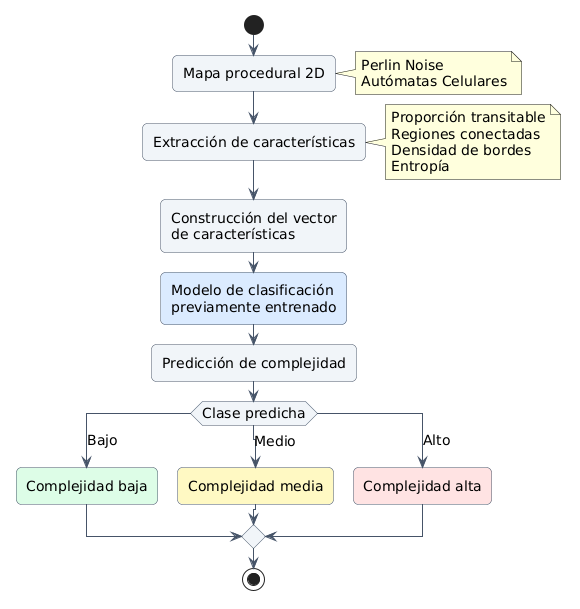
\includegraphics[
	width=0.85\textwidth,
	height=0.65\textheight,
	keepaspectratio
	]{imagenes/enfoque_clasificacion.png}
	\caption{Enfoque de clasificación supervisada
		de mapas en Rhyzome}
	\label{fig:enfoque_clasificacion}
\end{figure}

\FloatBarrier

Como se observa en la Figura~\ref{fig:enfoque_clasificacion}, el modelo de aprendizaje automático no interviene directamente en la construcción de las matrices de terreno. Su función consiste en analizar las características extraídas de los mapas generados y estimar su nivel de complejidad estructural. Esta separación permite mantener responsabilidades diferenciadas entre la generación procedural y la clasificación supervisada, conservando los algoritmos responsables de la construcción de los mapas y proporcionando información al mecanismo de selección adaptativa descrito en la Sección~\ref{sec:integracion_ia}.

% ============================================================
% 4.1.2 FORMULACIÓN DEL PROBLEMA DE CLASIFICACIÓN
% ============================================================

\subsection{Formulación del problema de clasificación}
\label{subsec:formulacion_clasificacion}

La clasificación de la complejidad estructural en Rhyzome se formula como un problema de aprendizaje supervisado multiclase, en el cual las propiedades cuantificables de un mapa constituyen las variables de entrada del modelo y el nivel de complejidad representa la variable objetivo.

Cada mapa se representa mediante un vector de características:

\begin{equation}
	\mathbf{x}=(x_1,x_2,\ldots,x_d)
	\label{eq:vector_caracteristicas}
\end{equation}

donde $d$ corresponde al número de características de entrada y cada $x_i$ representa una propiedad cuantificable del mapa, como la proporción de espacios transitables, la cantidad de regiones conectadas, la densidad de bordes o la entropía. Estas características permiten representar numéricamente la estructura del escenario generado.

El conjunto de clases de complejidad se define como:

\begin{equation}
	\mathcal{C}=\{\text{bajo},\text{medio},\text{alto}\}.
	\label{eq:clases_complejidad}
\end{equation}

A partir del vector de características, el modelo establece una relación entre las propiedades estructurales del mapa y las clases de complejidad definidas. La predicción se expresa mediante:

\begin{equation}
	\hat{y}=f_{\theta}(\mathbf{x}),\qquad f_{\theta}:\mathbb{R}^{d}\rightarrow\mathcal{C}.
	\label{eq:prediccion_complejidad}
\end{equation}

En esta expresión, $f_{\theta}$ representa la función de clasificación, $\theta$ corresponde a los parámetros aprendidos durante el entrenamiento y $\hat{y}$ representa la clase predicha para el mapa evaluado.

La dimensionalidad del vector de entrada depende de la configuración experimental utilizada. En el estudio de clasificadores especializados por familia de generación procedural se utilizaron diez características ($d=10$), mientras que la configuración experimental emplea ocho características ($d=8$).

La clasificación obtenida representa una estimación de la complejidad estructural del mapa y no equivale necesariamente a la dificultad percibida por un jugador, debido a que esta última puede depender de factores adicionales, como las mecánicas del videojuego, los objetivos y las habilidades del usuario. La predicción obtenida proporciona información al mecanismo de selección adaptativa de candidatos descrito en la Sección~\ref{sec:integracion_ia}.

% ============================================================
% 4.1.3 MODELOS DE CLASIFICACIÓN CONSIDERADOS
% ============================================================

\subsection{Modelos de clasificación considerados}
\label{subsec:modelos_considerados}

Para abordar el problema de clasificación de la complejidad estructural de mapas bidimensionales, se evaluaron seis algoritmos de aprendizaje supervisado pertenecientes a diferentes familias de modelos. La selección de estos clasificadores permitió establecer una comparación experimental entre enfoques lineales, métodos basados en instancias, ensambles de árboles de decisión, máquinas de vectores de soporte y redes neuronales artificiales.

La comparación permite examinar relaciones lineales y no lineales entre las características estructurales y los niveles de complejidad.

\textbf{Regresión Logística (LR).}
Es un algoritmo de clasificación que permite estimar la probabilidad de pertenencia de una observación a una determinada clase mediante una función basada en la combinación de las variables de entrada \parencite{james2023}.

\textbf{K-Nearest Neighbors (KNN).}
Es un algoritmo basado en instancias que realiza la clasificación de una observación a partir de las clases correspondientes a sus vecinos más próximos, identificados mediante medidas de distancia o similitud dentro del espacio de características \parencite{cunningham2021}.

\textbf{Random Forest (RF).}
Es un método de aprendizaje basado en un conjunto de árboles de decisión construidos mediante mecanismos de aleatoriedad, cuyas predicciones se combinan para obtener una clasificación \parencite{breiman2001}.

\textbf{Máquinas de vectores de soporte (SVM).}
Son modelos de aprendizaje supervisado orientados a establecer fronteras de decisión que maximicen el margen de separación entre clases \parencite{cortes1995}. Mediante el uso de una función kernel de base radial (RBF), es posible representar fronteras de decisión no lineales.

\textbf{Gradient Boosting (GB).}
Es una técnica de aprendizaje basada en la construcción secuencial de modelos, en la cual cada nuevo estimador contribuye a mejorar el desempeño del conjunto mediante la optimización de una función de pérdida \parencite{friedman2001}.

\textbf{Perceptrón multicapa (MLP).}
Es un modelo de red neuronal artificial compuesto por una capa de entrada, una o más capas ocultas y una capa de salida. Mediante funciones de activación no lineales y el ajuste de los pesos durante el entrenamiento, este modelo permite representar relaciones complejas entre las variables de entrada \parencite{goodfellow2016}.

La Tabla~\ref{tab:modelos_considerados} sintetiza los fundamentos de los seis clasificadores evaluados y la justificación de su incorporación dentro del proceso experimental de Rhyzome.

\begin{table}[htbp]
	\centering
	
	\caption{Modelos de clasificación considerados}
	\label{tab:modelos_considerados}
	
	\renewcommand{\arraystretch}{1.5}
	
	\begin{tabularx}{\textwidth}{
			|>{\raggedright\arraybackslash}p{3.5cm}|
			>{\raggedright\arraybackslash}X|
			>{\raggedright\arraybackslash}X|
		}
		
		\hline
		
		\rowcolor{gray!15}
		\textbf{Modelo} &
		\textbf{Fundamento} &
		\textbf{Justificación} \\
		
		\hline
		
		Regresión Logística (LR) &
		Clasificación probabilística mediante
		fronteras de decisión lineales. &
		Establecer una línea base interpretable
		para la comparación experimental. \\
		
		\hline
		
		KNN &
		Clasificación basada en la proximidad
		entre observaciones. &
		Evaluar la similitud estructural
		entre mapas. \\
		
		\hline
		
		Random Forest (RF) &
		Ensamble de árboles de decisión
		construidos mediante aleatoriedad. &
		Identificar relaciones no lineales
		e interacciones entre características. \\
		
		\hline
		
		SVM (RBF) &
		Fronteras de máximo margen mediante
		una función kernel de base radial. &
		Evaluar la separación no lineal
		de los niveles de complejidad. \\
		
		\hline
		
		Gradient Boosting (GB) &
		Construcción secuencial de estimadores
		mediante optimización de una función
		de pérdida. &
		Evaluar el aprendizaje progresivo
		de patrones estructurales. \\
		
		\hline
		
		Perceptrón multicapa (MLP) &
		Red neuronal artificial con múltiples
		capas y funciones de activación. &
		Evaluar interacciones complejas
		entre las variables de entrada. \\
		
		\hline
		
	\end{tabularx}
\end{table}

\FloatBarrier

La evaluación de estos seis clasificadores permite comparar diferentes estrategias de aprendizaje automático sin asumir previamente la superioridad de un algoritmo sobre los demás. La selección de los modelos se fundamenta en los resultados obtenidos durante el proceso experimental, considerando su capacidad para clasificar los niveles de complejidad estructural de los mapas.

Es importante distinguir entre los modelos considerados durante la experimentación y aquellos seleccionados para su integración en el prototipo. La configuración de entrenamiento, las métricas de evaluación y los resultados comparativos se presentan en las secciones posteriores de este capítulo, donde se establecen los criterios utilizados para justificar la selección de los modelos.


% ============================================================
% 4.2 DATASET: FUENTE, CARACTERÍSTICAS Y PREPROCESAMIENTO
% ============================================================

\section{Dataset: fuente, características y preprocesamiento}
\label{sec:dataset_ia}

La construcción del conjunto de datos constituye una etapa fundamental para el desarrollo del componente de aprendizaje automático de Rhyzome, debido a que las características estructurales de los mapas proporcionan la información necesaria para el entrenamiento y la evaluación de los modelos de clasificación.

La estrategia experimental contempla la generación de datos sintéticos mediante los algoritmos de generación procedural implementados en el proyecto, complementada con una fuente externa de niveles de videojuegos destinada a la comparación de sus propiedades estructurales.

% ============================================================
% 4.2.1 ORIGEN Y CONSTRUCCIÓN DEL DATASET
% ============================================================

\subsection{Origen y construcción del dataset}
\label{subsec:origen_dataset}

\textbf{Generación del conjunto de datos sintéticos.}

El conjunto de datos sintéticos se construyó mediante la generación de mapas bidimensionales utilizando los algoritmos Perlin Noise \parencite{perlin1985} y Autómatas Celulares \parencite{johnson2010}. La utilización de estos algoritmos permite obtener diferentes configuraciones estructurales mediante la modificación de sus parámetros de generación, conservando la posibilidad de reproducir los escenarios a partir de semillas.

El conjunto de datos del experimento documentado en el manifiesto experimental está compuesto por 10.000 mapas sintéticos, distribuidos uniformemente entre los cuatro tipos de terreno considerados en Rhyzome: bosque, desierto, ciudad y mazmorra. Cada tipo de terreno cuenta con 2.500 muestras, permitiendo incorporar diferentes configuraciones estructurales dentro del conjunto de datos.

La Tabla~\ref{tab:distribucion_dataset_sintetico} presenta la distribución de los mapas sintéticos según el tipo de terreno y el algoritmo de generación procedural utilizado.

\begin{table}[htbp]
	\centering
	
	\caption{Distribución del conjunto de datos sintéticos}
	\label{tab:distribucion_dataset_sintetico}
	
	\renewcommand{\arraystretch}{1.5}
	
	\begin{tabularx}{\textwidth}{
			|>{\raggedright\arraybackslash}X|
			>{\raggedright\arraybackslash}X|
			>{\centering\arraybackslash}p{2.3cm}|
			>{\centering\arraybackslash}p{2.3cm}|
		}
		
		\hline
		
		\rowcolor{gray!15}
		\textbf{Terreno} &
		\textbf{Algoritmo} &
		\textbf{Cantidad} &
		\textbf{Porcentaje} \\
		
		\hline
		
		Bosque &
		Perlin Noise &
		2.500 &
		25\% \\ \hline
		
		Desierto &
		Perlin Noise &
		2.500 &
		25\% \\ \hline
		
		Ciudad &
		Perlin Noise &
		2.500 &
		25\% \\ \hline
		
		Mazmorra &
		Autómatas Celulares &
		2.500 &
		25\% \\ \hline
		
		\rowcolor{gray!10}
		\textbf{Total} &
		--- &
		\textbf{10.000} &
		\textbf{100\%} \\
		
		\hline
		
	\end{tabularx}
\end{table}

\FloatBarrier

Como se observa en la Tabla~\ref{tab:distribucion_dataset_sintetico}, el algoritmo Perlin Noise representa el 75\% del conjunto
de datos, mientras que Autómatas Celulares representa el 25\% restante. Esta distribución se deriva de la asociación de los algoritmos con los tipos de terreno definidos en Rhyzome.

Las dimensiones de los mapas se seleccionaron de manera independiente para el ancho y el alto, utilizando valores comprendidos entre 24 y 100 celdas, en incrementos de cuatro. Esta variación permitió incorporar escenarios de diferentes dimensiones dentro del conjunto de datos experimental.

Para favorecer la reproducibilidad del proceso de generación se utilizaron tres bases de semillas: 420000, 1230000 y 20260000. A partir de estas bases y del índice de cada muestra se determinó la semilla individual utilizada para la generación del mapa.

Los perfiles de generación se configuraron de acuerdo con los niveles de complejidad solicitados: bajo, medio y alto. Para Perlin Noise se consideraron variaciones en el número de octavas, la persistencia y el umbral de generación. Para Autómatas Celulares se modificaron la probabilidad inicial de ocupación, el número de iteraciones y los límites de nacimiento y supervivencia de las celdas.

Cada registro experimental conserva un identificador, el tipo de terreno, el algoritmo de generación, las dimensiones, la semilla, los parámetros utilizados y las características estructurales extraídas del mapa.

La distribución por complejidad solicitada se presenta en la Tabla~\ref{tab:distribucion_dataset}.

\textbf{Incorporación de datos externos.}

Como fuente complementaria de información se utilizó The Video Game Level Corpus (VGLC), un repositorio académico que proporciona representaciones de niveles de videojuegos en formatos adecuados para su procesamiento computacional y su utilización en investigaciones relacionadas con inteligencia artificial y generación procedural de contenido \parencite{summerville2016}.

El repositorio oficial se encuentra disponible en:

\begin{center}
	\url{https://github.com/TheVGLC/TheVGLC}
\end{center}

Durante la experimentación se seleccionaron archivos de texto correspondientes a niveles de The Legend of Zelda. A partir de estos archivos se extrajeron 200 ventanas bidimensionales de $32 \times 32$ celdas.

El procedimiento de transformación de los niveles externos comprendió las siguientes actividades:

\begin{enumerate}
	
	\item Descarga del repositorio VGLC desde su rama
	principal denominada \texttt{master}.
	
	\item Selección de los archivos de texto asociados
	a The Legend of Zelda.
	
	\item Conversión de los niveles a matrices binarias,
	considerando los caracteres \texttt{X}, \texttt{\#}
	y \texttt{W} como obstáculos y los demás caracteres
	como espacios transitables.
	
	\item Aplicación de relleno con obstáculos cuando las
	dimensiones originales eran inferiores al tamaño
	requerido de la ventana.
	
	\item Extracción de ventanas de $32 \times 32$ celdas
	mediante desplazamientos de 16 celdas.
	
	\item Selección de ventanas cuya proporción de espacio
	transitable se encontrara entre el 5\% y el 95\%.
	
	\item Extracción de las características estructurales
	de las 200 ventanas seleccionadas.
	
\end{enumerate}

La Tabla~\ref{tab:dataset_externo_vglc} sintetiza las principales características del conjunto de datos externo.

\begin{table}[htbp]
	\centering
	
	\caption{Características del conjunto de datos externo VGLC}
	\label{tab:dataset_externo_vglc}
	
	\renewcommand{\arraystretch}{1.5}
	
	\begin{tabularx}{\textwidth}{
			|>{\raggedright\arraybackslash}p{5cm}|
			>{\raggedright\arraybackslash}X|
		}
		
		\hline
		
		\rowcolor{gray!15}
		\textbf{Característica} &
		\textbf{Descripción} \\
		
		\hline
		
		Fuente &
		The Video Game Level Corpus (VGLC) \\ \hline
		
		Videojuego de procedencia &
		The Legend of Zelda \\ \hline
		
		Formato original &
		Archivos de texto \\ \hline
		
		Cantidad de muestras &
		200 ventanas \\ \hline
		
		Dimensiones &
		$32 \times 32$ celdas \\ \hline
		
		Desplazamiento entre ventanas &
		16 celdas \\ \hline
		
		Representación procesada &
		Matriz binaria \\ \hline
		
		Participación en el entrenamiento &
		No \\ \hline
		
		Evaluación de métricas de clasificación &
		No \\ \hline
		
		Finalidad experimental &
		Comparación de distribuciones estructurales \\
		
		\hline
		
	\end{tabularx}
\end{table}

\FloatBarrier

Las muestras externas se mantuvieron separadas del entrenamiento y de la evaluación supervisada. Al no disponer de etiquetas de complejidad equivalentes a las de Rhyzome, no se utilizaron para calcular exactitud, precisión, sensibilidad ni F1. Su finalidad fue comparar distribuciones de propiedades estructurales, no validar de manera supervisada el desempeño predictivo.


\textbf{Trazabilidad y reproducibilidad del conjunto de datos.}

El proceso experimental contempla la exportación de los registros de los mapas sintéticos en formato CSV, así como de sus representaciones individuales en formatos JSON y PNG. Los archivos JSON conservan las matrices binarias, las semillas, las dimensiones, los parámetros de generación y las características estructurales de cada mapa, mientras que el manifiesto experimental registra la cantidad de muestras, su distribución por algoritmo y tipo de terreno, las características utilizadas por los clasificadores y la configuración de evaluación. En conjunto, estos elementos
permiten establecer la trazabilidad entre los datos generados, el proceso de entrenamiento y los artefactos de aprendizaje automático obtenidos, facilitando la reproducción de las condiciones experimentales.

En cuanto al conjunto de datos externo, el procedimiento de descarga utilizó la rama \texttt{master} del repositorio VGLC sin registrar el identificador específico del commit ni conservar en las evidencias disponibles un listado individual de los archivos de procedencia. Esta situación constituye una limitación para reproducir exactamente la selección de las muestras externas en ejecuciones posteriores, debido a las posibles modificaciones en el contenido del repositorio. No obstante, la documentación del procedimiento de extracción, transformación y selección de
las ventanas permite reproducir la metodología empleada para la construcción del conjunto de datos externo.

\FloatBarrier


\subsection{Características estructurales de los mapas}
\label{subsec:caracteristicas_estructurales}

La extracción de características constituye el mecanismo mediante el cual los mapas bidimensionales se transforman en representaciones numéricas adecuadas para su procesamiento mediante algoritmos de aprendizaje automático. En Rhyzome, estas características describen la distribución espacial de las celdas transitables, la fragmentación de las regiones, las transiciones entre obstáculos y espacios abiertos, así como la variabilidad estructural de los escenarios. Su definición, cálculo y orden deben mantenerse consistentes entre las etapas de entrenamiento e inferencia, garantizando que las variables suministradas a los clasificadores conserven el mismo significado.

\textbf{Representación binaria de los mapas.}

Para realizar la extracción de características, cada mapa se representa mediante una matriz binaria $M$ de dimensiones $H \times W$, donde $H$ corresponde al número de filas y $W$ al número de columnas. Cada elemento $m_{ij}$ representa el estado de una celda según la siguiente convención:

\begin{equation}
	M \in \{0,1\}^{H \times W},
	\qquad
	m_{ij} =
	\begin{cases}
		1, & \text{si la celda es transitable},\\
		0, & \text{si la celda es un obstáculo}.
	\end{cases}
	\label{eq:representacion_binaria_ml}
\end{equation}

La matriz de colisiones utilizada por Rhyzome presenta una codificación inversa, en la cual el valor cero representa una celda transitable y el valor uno representa un obstáculo. Para garantizar la correspondencia con la representación requerida por el extractor de características, el adaptador de aprendizaje automático realiza una transformación binaria antes de procesar el mapa. Esta operación conserva las dimensiones y la distribución espacial de las celdas, modificando únicamente su codificación mediante la expresión:

\begin{equation}
	m_{ij}=1-c_{ij},
	\label{eq:conversion_collision_ml}
\end{equation}

donde $c_{ij}$ representa el valor de la celda ubicada en la posición $(i,j)$ de la matriz de colisiones.

La Figura~\ref{fig:representacion_estructural_mapas} presenta un ejemplo del procedimiento de transformación y extracción de características estructurales implementado en Rhyzome. El diagrama parte de una matriz de colisiones de dimensiones $5 \times 5$, muestra su conversión al formato requerido por el componente de aprendizaje automático y representa la identificación de regiones transitables, junto con el cálculo de tres características utilizadas por los clasificadores.

\begin{figure}[htbp]
	\centering
	
	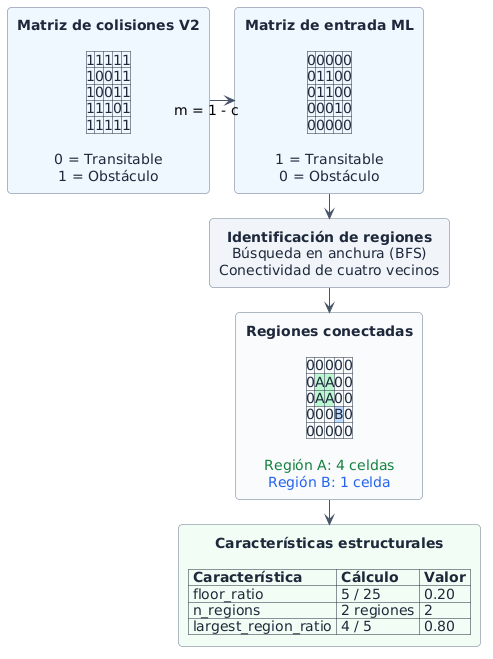
\includegraphics[
	width=0.85\textwidth,
	height=0.75\textheight,
	keepaspectratio
	]{imagenes/representacion_estructural_mapas.png}
	
	\caption{Representación binaria y extracción de características estructurales en Rhyzome}
	
	\label{fig:representacion_estructural_mapas}
\end{figure}

\FloatBarrier

Como se observa en la figura, el procedimiento comienza con la conversión de la matriz de colisiones a una representación en la cual las celdas transitables adquieren el valor uno. Posteriormente, se aplica un algoritmo de búsqueda en anchura (\textit{Breadth-First Search}, BFS) para identificar las regiones transitables mediante una conectividad de cuatro vecinos. En el ejemplo se obtienen dos regiones independientes, identificadas como A y B, conformadas por cuatro y una celda, respectivamente. Aunque ambas regiones presentan proximidad diagonal, permanecen separadas debido a que el criterio de conectividad considera únicamente las relaciones de adyacencia horizontal y vertical.

A partir de la información obtenida se calculan las características \texttt{floor\_ratio}, \texttt{n\_regions} y \texttt{largest\_region\_ratio}. La primera corresponde a la proporción de celdas transitables respecto al total de la matriz, obteniendo un valor de $0.20$ a partir de cinco celdas transitables de un total de veinticinco. La segunda registra las dos regiones conectadas identificadas, mientras que la tercera representa la proporción del espacio transitable perteneciente a la región de mayor tamaño, cuyo resultado es $0.80$, correspondiente a cuatro de las cinco celdas transitables.

El escenario presentado constituye un ejemplo ilustrativo de elaboración propia y no corresponde a una muestra del conjunto de datos experimental. Su propósito es facilitar la comprensión de la relación entre la representación binaria del mapa y las características numéricas utilizadas por el componente de aprendizaje automático. Si bien la figura presenta únicamente tres características, el extractor también calcula propiedades relacionadas con la densidad de bordes, la entropía por filas y columnas, la varianza local y la relación entre perímetro y área transitable, cuyas definiciones matemáticas se desarrollan a continuación.


\subsection{Etiquetado de los niveles de complejidad}

El etiquetado de los niveles de complejidad constituye una etapa fundamental en la construcción del conjunto de datos, puesto que establece las categorías que el componente de aprendizaje supervisado debe reconocer a partir de las características estructurales de los mapas. En Rhyzome se definen tres categorías de complejidad: baja, media y alta, asociadas a perfiles generativos que modifican los parámetros utilizados durante la construcción procedural de los escenarios.

El procedimiento experimental distingue entre la complejidad solicitada y la complejidad observada. La primera corresponde al perfil generativo seleccionado antes de construir el mapa y constituye la variable objetivo del entrenamiento. La segunda se obtiene mediante un índice auxiliar calculado a partir de las propiedades estructurales del escenario generado, con el propósito de analizar la correspondencia entre los parámetros de generación y las características resultantes.

\textbf{Asignación de etiquetas mediante perfiles generativos.}

La asignación de etiquetas se realiza mediante reglas predefinidas de generación y no mediante una clasificación manual de los mapas por parte de expertos o jugadores. Cada muestra conserva el nivel de complejidad solicitado en la variable \texttt{complexity\_requested}, cuyo dominio se encuentra definido por la expresión:

\begin{equation}
	y_{\mathrm{sol}} \in
	\{\mathrm{bajo},\mathrm{medio},\mathrm{alto}\}
	\label{eq:complejidad_solicitada}
\end{equation}

En el experimento de clasificación especializada por familia procedural, los perfiles generativos establecen intervalos de variación para los parámetros de Perlin Noise y Autómatas Celulares. En el caso de Perlin Noise se consideran el número de octavas, la persistencia y el umbral de generación, mientras que para Autómatas Celulares se modifican la probabilidad inicial de ocupación, el número de iteraciones y los límites asociados a las reglas de nacimiento y supervivencia.

En el experimento de clasificación unificada de Rhyzome V2, los perfiles se definen de manera independiente para cada bioma, considerando sus características semánticas y los elementos que intervienen en la construcción de la capa de colisiones. Esta configuración permite establecer diferentes condiciones de generación para los escenarios de bosque, desierto, ciudad y mazmorra.

La Tabla~\ref{tab:perfiles_complejidad_v2} presenta los valores definidos para cada perfil experimental en Rhyzome.

\begin{table}[htbp]
	\centering
	
	\caption{Parámetros de los perfiles generativos de complejidad en Rhyzome}
	
	\label{tab:perfiles_complejidad_v2}
	
	\renewcommand{\arraystretch}{1.5}
	
	\begin{tabularx}{\textwidth}{
			|>{\raggedright\arraybackslash}p{2cm}|
			>{\raggedright\arraybackslash}X|
			>{\centering\arraybackslash}p{1.3cm}|
			>{\centering\arraybackslash}p{1.3cm}|
			>{\centering\arraybackslash}p{1.3cm}|
		}
		
		\hline
		
		\rowcolor{gray!15}
		\textbf{Bioma} &
		\textbf{Parámetro} &
		\textbf{Bajo} &
		\textbf{Medio} &
		\textbf{Alto} \\ \hline
		
		Bosque &
		Umbral de agua &
		0,10 & 0,17 & 0,24 \\ \hline
		
		Bosque &
		Probabilidad de árboles &
		0,15 & 0,31 & 0,45 \\ \hline
		
		Bosque &
		Probabilidad de rocas &
		0,015 & 0,035 & 0,06 \\ \hline
		
		Desierto &
		Umbral de agua &
		0,06 & 0,12 & 0,18 \\ \hline
		
		Desierto &
		Probabilidad de cactus &
		0,04 & 0,09 & 0,16 \\ \hline
		
		Desierto &
		Probabilidad de rocas &
		0,02 & 0,04 & 0,07 \\ \hline
		
		Ciudad &
		Probabilidad de edificios &
		0,45 & 0,73 & 0,90 \\ \hline
		
		Ciudad &
		Probabilidad de árboles &
		0,01 & 0,025 & 0,05 \\ \hline
		
		Mazmorra &
		Probabilidad inicial de muros &
		0,38 & 0,43 & 0,49 \\ \hline
		
		Mazmorra &
		Número de iteraciones &
		3 & 4 & 6 \\ \hline
		
	\end{tabularx}
	
\end{table}

\FloatBarrier

Los parámetros presentados constituyen hipótesis experimentales orientadas a producir diferencias estructurales entre los niveles de complejidad. En los biomas de bosque y desierto se modifican las condiciones de aparición de agua y objetos que restringen el desplazamiento. En ciudad se modifica la probabilidad de aparición de edificios y árboles, mientras que en
mazmorra se ajustan la probabilidad inicial de muros y el número de iteraciones del autómata celular.

La generación semántica de Rhyzome V2 utiliza ruido suave mediante interpolación bilineal para bosque y desierto, reglas de distribución espacial para ciudad y autómatas celulares para mazmorra. Posteriormente, la variante optimizada incorpora modificaciones orientadas a mejorar la conectividad o preservar accesos transitables, dependiendo del bioma. Por consiguiente, los parámetros generativos condicionan la estructura del escenario, pero no garantizan por sí mismos un incremento monotónico de todas las características asociadas a la complejidad.

Durante la construcción del conjunto de datos de clasificación unificada se consideran doce combinaciones experimentales, correspondientes a cuatro biomas y tres niveles de complejidad. Los mapas se generan con dimensiones constantes de $50 \times 35$ celdas, utilizando la variante optimizada B y reutilizando la misma secuencia de semillas entre perfiles. La predicción mediante aprendizaje automático permanece desactivada durante este procedimiento, de manera que la etiqueta almacenada corresponde exclusivamente al perfil solicitado y no a la salida de un clasificador.

\textbf{Índice auxiliar de complejidad estructural.}

Como mecanismo complementario de análisis, en el experimento de clasificación especializada se construye un índice de complejidad estructural denominado \texttt{complexity\_score}. Su propósito consiste en cuantificar propiedades relacionadas con la variabilidad, el detalle y la fragmentación de los escenarios, permitiendo analizar la correspondencia entre los
perfiles generativos y las estructuras obtenidas.

El índice considera seis de las características estructurales descritas en la Subsección~\ref{subsec:caracteristicas_estructurales}: densidad de bordes, varianza local, entropía por filas, entropía por columnas, relación entre perímetro y área transitable, y número de regiones conectadas.

Debido a que estas características presentan diferentes escalas y rangos de valores, se aplica una normalización robusta basada en los percentiles 5 y 95 del conjunto de datos. Para cada característica $j$ de la muestra $i$, el valor normalizado se obtiene mediante:

\begin{equation}
	z_{ij} =
	\min\left(
	1,
	\max\left(
	0,
	\frac{x_{ij}-P_{5,j}}
	{P_{95,j}-P_{5,j}+\varepsilon}
	\right)
	\right)
	\label{eq:normalizacion_complejidad}
\end{equation}

donde $x_{ij}$ representa el valor original de la característica, $P_{5,j}$ y $P_{95,j}$ corresponden a los percentiles 5 y 95, respectivamente, y $\varepsilon=10^{-12}$ constituye una constante numérica que evita la división por cero.

La restricción de los valores normalizados al intervalo $[0,1]$ limita la influencia de las observaciones extremas. Posteriormente, el índice estructural se calcula mediante el promedio aritmético de las seis características normalizadas, escalado al intervalo $[0,100]$ y redondeado a dos posiciones decimales:

\begin{equation}
	S_i =
	\operatorname{round}
	\left(
	\frac{100}{6}
	\sum_{j=1}^{6} z_{ij},
	2
	\right)
	\label{eq:indice_complejidad_estructural}
\end{equation}

donde $S_i$ representa el índice de complejidad estructural correspondiente al mapa $i$. La formulación asigna la misma ponderación a los seis indicadores, sin establecer prioridades entre ellos.

El índice constituye una medida compuesta definida para los propósitos experimentales de Rhyzome. Su interpretación depende de las características seleccionadas, del procedimiento de normalización y de la distribución del conjunto de datos utilizado.

\textbf{Determinación de la complejidad observada.}

A partir de los valores obtenidos mediante el índice estructural, se establecen dos umbrales empíricos correspondientes a los cuantiles de orden $1/3$ y $2/3$ de su distribución:

\begin{equation}
	q_1 = Q_S\left(\frac{1}{3}\right),
	\qquad
	q_2 = Q_S\left(\frac{2}{3}\right)
	\label{eq:terciles_complejidad}
\end{equation}

donde $Q_S$ representa la función de cuantiles asociada a la distribución del índice estructural.

La complejidad observada, almacenada en la variable \texttt{complexity\_observed}, se determina mediante la siguiente función de clasificación:

\begin{equation}
	y_{\mathrm{obs},i} =
	\begin{cases}
		\mathrm{bajo}, & S_i \leq q_1,\\
		\mathrm{medio}, & q_1 < S_i \leq q_2,\\
		\mathrm{alto}, & S_i > q_2.
	\end{cases}
	\label{eq:complejidad_observada}
\end{equation}

Los resultados registrados en el notebook experimental establecen valores de aproximadamente $37{,}10$ y $54{,}81$ puntos para los umbrales $q_1$ y $q_2$, respectivamente. La Tabla~\ref{tab:umbrales_complejidad_observada} presenta los intervalos resultantes.

\begin{table}[htbp]
	\centering
	
	\caption{Umbrales empíricos de complejidad estructural observada}
	
	\label{tab:umbrales_complejidad_observada}
	
	\renewcommand{\arraystretch}{1.5}
	
	\begin{tabularx}{\textwidth}{
			|>{\raggedright\arraybackslash}p{3cm}|
			>{\centering\arraybackslash}X|
			>{\raggedright\arraybackslash}X|
		}
		
		\hline
		
		\rowcolor{gray!15}
		\textbf{Complejidad} &
		\textbf{Intervalo aproximado} &
		\textbf{Interpretación} \\ \hline
		
		Baja &
		$0 \leq S_i \leq 37{,}10$ &
		Tercio inferior de la distribución
		estructural. \\ \hline
		
		Media &
		$37{,}10 < S_i \leq 54{,}81$ &
		Tercio intermedio de la distribución
		estructural. \\ \hline
		
		Alta &
		$54{,}81 < S_i \leq 100$ &
		Tercio superior de la distribución
		estructural. \\ \hline
		
	\end{tabularx}
	
\end{table}

\FloatBarrier

Los umbrales obtenidos son específicos del conjunto de datos experimental y no constituyen límites universales de complejidad. Asimismo, la utilización de terciles establece una clasificación relativa respecto a la distribución analizada, por lo que
sus valores pueden variar ante modificaciones en los perfiles generativos, las dimensiones de los mapas o las características consideradas.

La Figura~\ref{fig:etiquetado_complejidad} presenta el procedimiento de asignación de etiquetas y cálculo de la complejidad observada, diferenciando la variable objetivo utilizada durante el entrenamiento del mecanismo auxiliar de análisis estructural.

\begin{figure}[htbp]
	\centering
	
	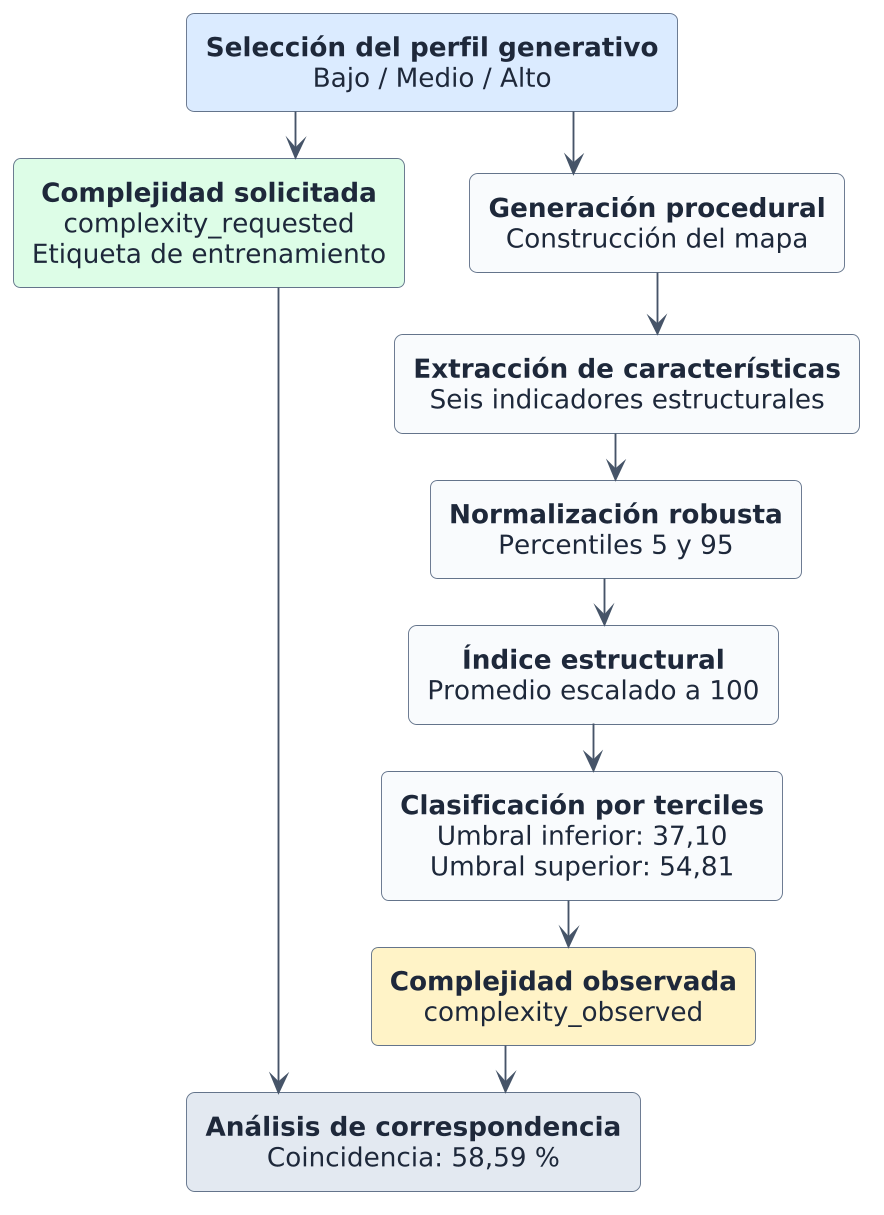
\includegraphics[
	width=0.90\textwidth,
	height=0.75\textheight,
	keepaspectratio
	]{imagenes/etiquetado_complejidad.png}
	
	\caption{Procedimiento experimental de etiquetado y análisis de complejidad estructural en Rhyzome}
	
	\label{fig:etiquetado_complejidad}
	
\end{figure}

\FloatBarrier

Como se observa en la figura, la complejidad solicitada se conserva como etiqueta desde el momento en que se selecciona el perfil generativo. Una vez construido el mapa, se extraen sus características estructurales y se calcula el índice auxiliar, a partir del cual se determina la complejidad observada mediante los umbrales empíricos. Ambos resultados se comparan para
analizar la correspondencia entre la configuración generativa y la estructura obtenida, sin sustituir la etiqueta utilizada durante el entrenamiento.

\textbf{Correspondencia entre complejidad solicitada y observada.}

Para analizar la correspondencia entre las dos representaciones de complejidad, se calcula la proporción de muestras cuya categoría solicitada coincide con la categoría observada:

\begin{equation}
	C =
	\frac{100}{N}
	\sum_{i=1}^{N}
	\mathbb{I}
	\left(
	y_{\mathrm{sol},i}
	=
	y_{\mathrm{obs},i}
	\right)
	\label{eq:coincidencia_complejidad}
\end{equation}

donde $N$ corresponde al número total de mapas analizados y $\mathbb{I}(\cdot)$ representa una función indicadora que toma el valor uno cuando ambas categorías coinciden y cero en caso contrario.

El resultado registrado para los 10.000 mapas del experimento de clasificación especializada fue de 58,59\% , equivalente a 5.859 muestras en las que la complejidad solicitada coincide con la complejidad observada mediante el índice estructural.

Este resultado evidencia que existe una correspondencia parcial entre los perfiles generativos y las propiedades estructurales consideradas, aunque también se presenta un solapamiento entre las categorías. El porcentaje obtenido no corresponde a una métrica de exactitud de aprendizaje automático, puesto que no se comparan predicciones de un clasificador, sino dos mecanismos de categorización definidos durante la construcción y el análisis del conjunto de datos.

\textbf{Codificación de las categorías de complejidad.}

Para su procesamiento mediante los algoritmos de aprendizaje supervisado, las categorías textuales se transforman en identificadores numéricos. La codificación utilizada depende del procedimiento experimental y del contrato de entrada y salida
asociado a cada modelo.

La Tabla~\ref{tab:codificacion_complejidad} presenta las correspondencias utilizadas durante la evaluación global del notebook, la exportación de los clasificadores especializados por familia procedural y el entrenamiento del clasificador
unificado de Rhyzome.

\begin{table}[htbp]
	\centering
	
	\caption{Codificación numérica de las categorías de complejidad por configuración experimental}
	
	\label{tab:codificacion_complejidad}
	
	\renewcommand{\arraystretch}{1.5}
	
	\begin{tabularx}{\textwidth}{
			|>{\raggedright\arraybackslash}p{2.3cm}|
			>{\centering\arraybackslash}X|
			>{\centering\arraybackslash}X|
			>{\centering\arraybackslash}X|
		}
		
		\hline
		
		\rowcolor{gray!15}
		\textbf{Complejidad} &
		\textbf{Evaluación global} &
		\textbf{Clasificación especializada} &
		\textbf{Clasificación unificada V2} \\ \hline
		
		Baja & 0 & 1 & 0 \\ \hline
		
		Media & 1 & 2 & 1 \\ \hline
		
		Alta & 2 & 0 & 2 \\ \hline
		
	\end{tabularx}
	
\end{table}

\FloatBarrier

Los identificadores numéricos representan categorías discretas y no magnitudes del índice estructural. Por consiguiente, las codificaciones no son intercambiables y deben conservarse de manera consistente durante el entrenamiento, la exportación
de los modelos y su integración con la aplicación. La interpretación de las predicciones requiere utilizar la correspondencia específica del modelo seleccionado.

\textbf{Alcance y limitaciones del etiquetado.}

El procedimiento adoptado permite construir un conjunto de datos etiquetado de manera reproducible, sin requerir una clasificación manual de cada mapa. Sin embargo, las etiquetas representan perfiles generativos definidos experimentalmente y no una valoración independiente de la dificultad percibida por los jugadores.

El índice auxiliar utiliza características que también forman parte de las variables de entrada de los clasificadores. Por esta razón, no constituye una referencia independiente para validar la capacidad predictiva de los modelos. No obstante,
dicho índice no se utiliza como variable objetivo ni como característica adicional de entrenamiento, evitando que el clasificador aprenda directamente la regla matemática utilizada para construir la complejidad observada.

En consecuencia, el alcance del aprendizaje supervisado se circunscribe al reconocimiento de perfiles generativos a partir de las propiedades estructurales de los mapas. La validación de una relación entre estas categorías y la dificultad jugable requeriría incorporar evaluaciones independientes, tales como estudios con jugadores, valoraciones de expertos o indicadores de desempeño durante la interacción con los escenarios.



\subsection{Distribución y composición del dataset}
\label{subsec:distribucion_dataset}

La composición del conjunto de datos constituye un aspecto relevante para el entrenamiento y la evaluación de los modelos de aprendizaje supervisado, puesto que la representación de las categorías y los tipos de escenarios condiciona las características disponibles durante el proceso de aprendizaje. En Rhyzome se establece una distribución aproximadamente equilibrada entre los niveles de complejidad solicitados, tanto en el experimento de clasificación especializada por familia procedural como en el experimento de clasificación unificada.

Cada procedimiento experimental dispone de un conjunto de 10.000 mapas sintéticos, construidos bajo condiciones generativas particulares. Aunque ambos conjuntos comparten las categorías de complejidad baja, media y alta, presentan diferencias en los mecanismos de generación, las dimensiones de los escenarios y las variables utilizadas durante el entrenamiento. Por consiguiente, su composición se analiza de manera independiente.

\textbf{Distribución del conjunto de datos de clasificación especializada.}

El conjunto de datos utilizado para la clasificación especializada se encuentra conformado por 10.000 mapas generados mediante Perlin Noise y Autómatas Celulares. La distribución comprende cuatro tipos de terreno: bosque, desierto, ciudad y mazmorra, con 2.500 muestras por cada uno.

La Tabla~\ref{tab:distribucion_dataset} presenta la distribución de las muestras según la familia procedural y el nivel de complejidad solicitado.

\begin{table}[htbp]
	\centering
	
	\caption{Distribución de muestras por familia procedural y complejidad solicitada}
	
	\label{tab:distribucion_dataset}
	
	\renewcommand{\arraystretch}{1.5}
	
	\begin{tabularx}{\textwidth}{
			|>{\raggedright\arraybackslash}X|
			>{\centering\arraybackslash}p{1.5cm}|
			>{\centering\arraybackslash}p{1.5cm}|
			>{\centering\arraybackslash}p{1.5cm}|
			>{\centering\arraybackslash}p{1.5cm}|
		}
		
		\hline
		
		\rowcolor{gray!15}
		\textbf{Familia procedural} &
		\textbf{Bajo} &
		\textbf{Medio} &
		\textbf{Alto} &
		\textbf{Total} \\ \hline
		
		Perlin Noise &
		2.502 & 2.499 & 2.499 & 7.500 \\ \hline
		
		Autómatas Celulares &
		834 & 833 & 833 & 2.500 \\ \hline
		
		\rowcolor{gray!10}
		\textbf{Total} &
		\textbf{3.336} &
		\textbf{3.332} &
		\textbf{3.332} &
		\textbf{10.000} \\ \hline
		
	\end{tabularx}
	
\end{table}

\FloatBarrier

La distribución por nivel de complejidad solicitada corresponde al 33,36\% para la categoría baja y al 33,32\% para cada una de las categorías media y alta. Esta composición proporciona una representación aproximadamente uniforme de las tres clases, tanto en el conjunto global como dentro de cada familia procedural.

En contraste, la distribución por familia procedural presenta una relación de tres a uno, debido a que Perlin Noise se utiliza para la generación de bosque, desierto y ciudad, mientras que Autómatas Celulares se emplea para la generación de mazmorras. Esta diferencia responde al diseño experimental y a la
asociación establecida entre los algoritmos y los tipos de terreno.

La Figura~\ref{fig:distribucion_dataset_especializado} representa gráficamente la distribución de las muestras por familia procedural y nivel de complejidad solicitado.

\begin{figure}[htbp]
	\centering
	
	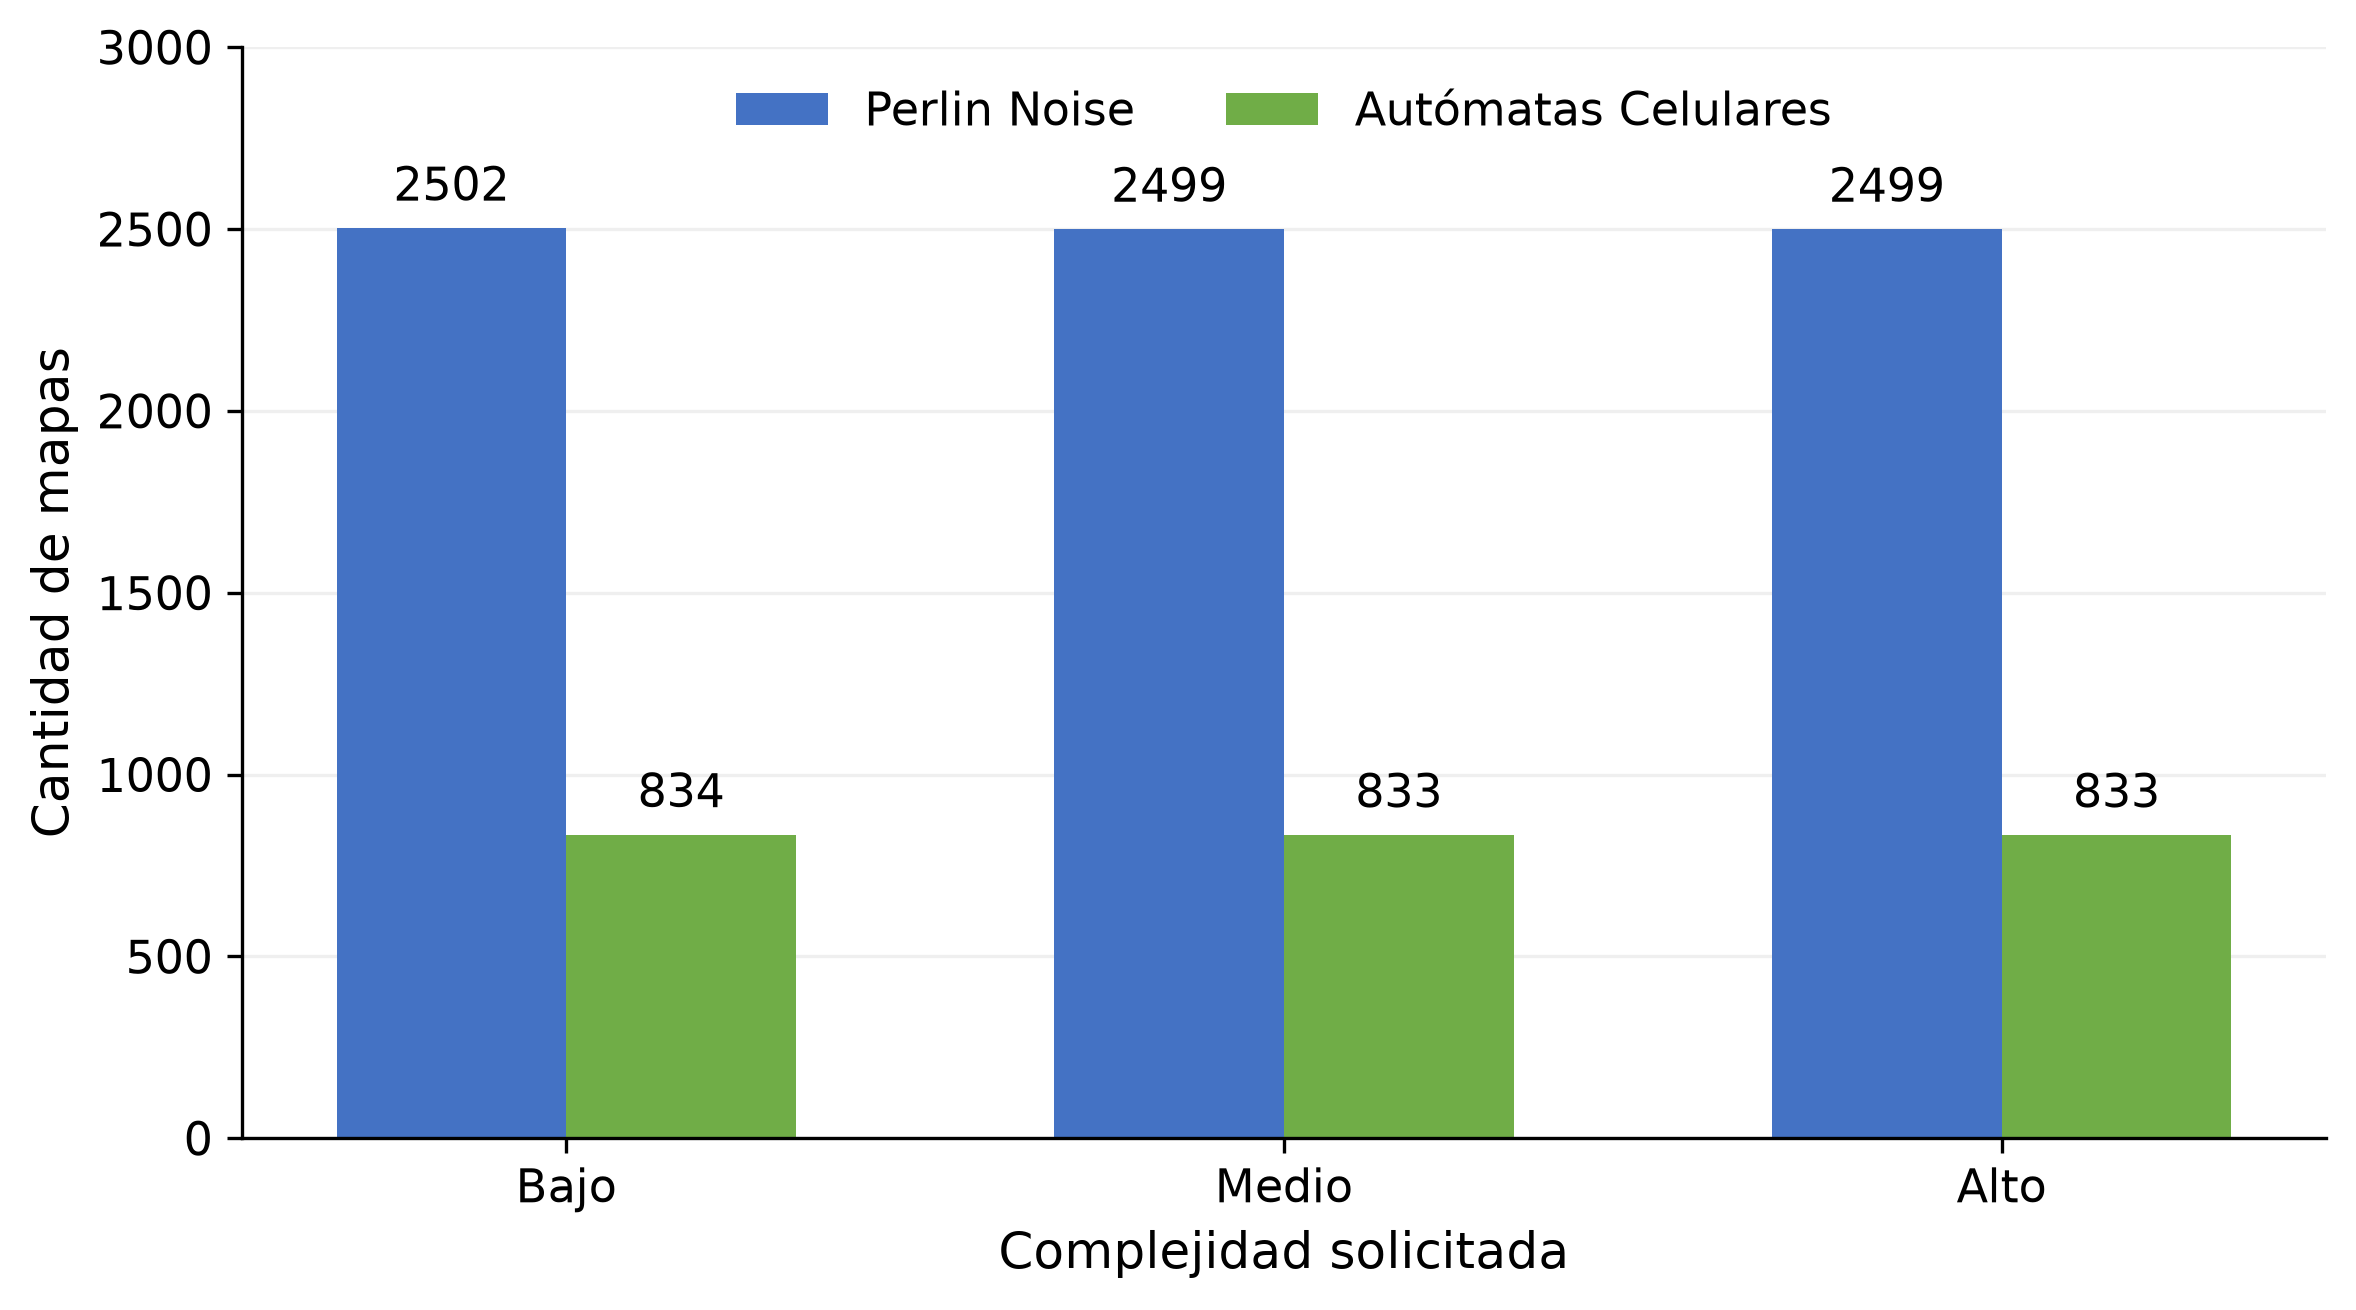
\includegraphics[
	width=0.90\textwidth,
	height=0.55\textheight,
	keepaspectratio
	]{imagenes/distribucion_dataset_especializado.png}
	
	\caption{Distribución de muestras por familia procedural y nivel de complejidad}
	
	\label{fig:distribucion_dataset_especializado}
	
\end{figure}

\FloatBarrier

La distribución presentada permite identificar que, aunque las familias procedurales disponen de diferentes cantidades de muestras, cada una conserva una representación aproximadamente equilibrada de las categorías de complejidad. Esta condición resulta relevante para la evaluación de los clasificadores
especializados, debido a que cada modelo se entrena sobre las muestras correspondientes a su familia procedural.

\textbf{Distribución del conjunto de datos de clasificación unificada.}

El conjunto de datos utilizado para la clasificación unificada de Rhyzome se construye a partir de doce combinaciones experimentales, correspondientes a cuatro biomas y tres niveles de complejidad. La distribución de las muestras se realiza mediante una asignación aproximadamente uniforme entre las combinaciones, utilizando la variante generativa optimizada B.

La Tabla~\ref{tab:distribucion_dataset_unificado} presenta los resultados obtenidos mediante el análisis del archivo \texttt{dataset\_v2\_10000.csv}.

\begin{table}[htbp]
	\centering
	
	\caption{Distribución de muestras por bioma y complejidad solicitada en Rhyzome}
	
	\label{tab:distribucion_dataset_unificado}
	
	\renewcommand{\arraystretch}{1.5}
	
	\begin{tabularx}{\textwidth}{
			|>{\raggedright\arraybackslash}X|
			>{\centering\arraybackslash}p{1.5cm}|
			>{\centering\arraybackslash}p{1.5cm}|
			>{\centering\arraybackslash}p{1.5cm}|
			>{\centering\arraybackslash}p{1.5cm}|
		}
		
		\hline
		
		\rowcolor{gray!15}
		\textbf{Bioma} &
		\textbf{Bajo} &
		\textbf{Medio} &
		\textbf{Alto} &
		\textbf{Total} \\ \hline
		
		Bosque &
		834 & 834 & 834 & 2.502 \\ \hline
		
		Desierto &
		834 & 833 & 833 & 2.500 \\ \hline
		
		Ciudad &
		833 & 833 & 833 & 2.499 \\ \hline
		
		Mazmorra &
		833 & 833 & 833 & 2.499 \\ \hline
		
		\rowcolor{gray!10}
		\textbf{Total} &
		\textbf{3.334} &
		\textbf{3.333} &
		\textbf{3.333} &
		\textbf{10.000} \\ \hline
		
	\end{tabularx}
	
\end{table}

\FloatBarrier

La distribución obtenida corresponde al 33,34\% para la categoría baja y al 33,33\% para cada una de las categorías media y alta. Las diferencias en las cantidades de muestras se derivan de la distribución del total de registros entre las doce combinaciones experimentales, sin representar un desequilibrio
significativo entre las clases o los biomas.

La Figura~\ref{fig:distribucion_dataset_unificado} presenta gráficamente la composición del conjunto de datos utilizado para el entrenamiento del clasificador unificado.

\begin{figure}[htbp]
	\centering
	
	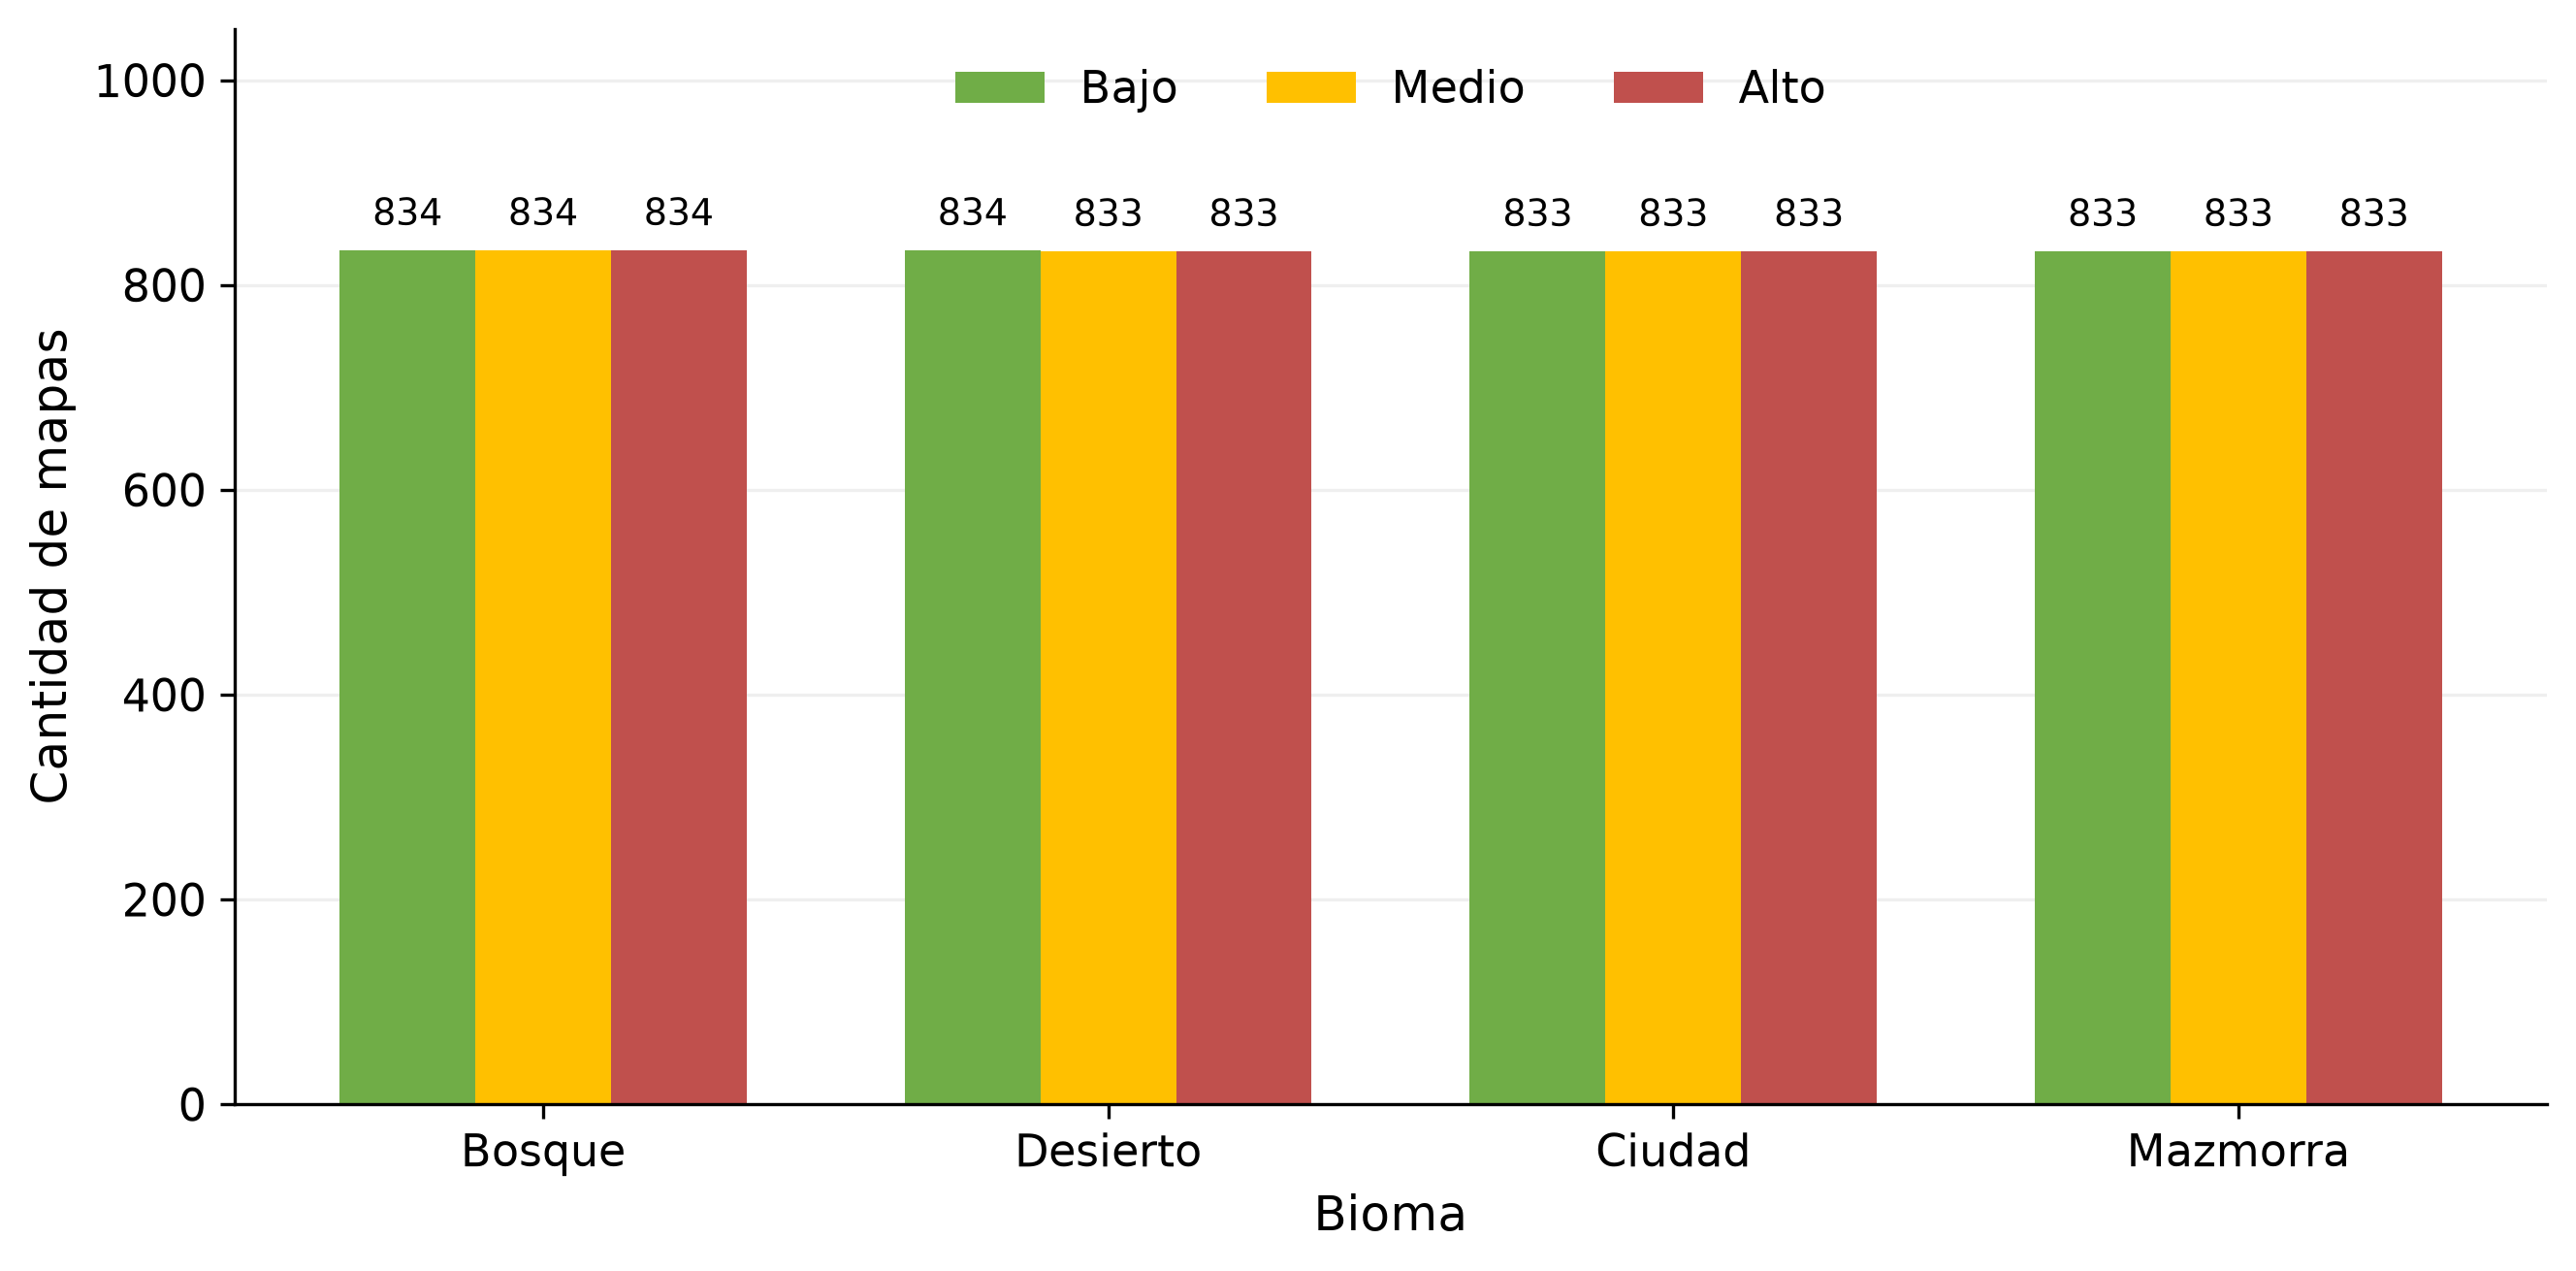
\includegraphics[
	width=0.90\textwidth,
	height=0.55\textheight,
	keepaspectratio
	]{imagenes/distribucion_dataset_unificado.png}
	
	\caption{Distribución de muestras por bioma	y nivel de complejidad en Rhyzome}
	
	\label{fig:distribucion_dataset_unificado}
	
\end{figure}

\FloatBarrier

A diferencia del enfoque especializado, la clasificación unificada utiliza un único conjunto de datos que incorpora los cuatro biomas. Esta composición permite evaluar la capacidad de los clasificadores para reconocer los perfiles de complejidad a partir de las características estructurales, considerando escenarios construidos mediante diferentes mecanismos generativos.

\textbf{Composición del conjunto de datos externo.}

Como complemento del experimento de clasificación especializada, se dispone de 200 muestras externas obtenidas a partir de niveles de The Legend of Zelda, pertenecientes al repositorio The Video Game Level Corpus (VGLC), cuyo procedimiento de extracción se describe en la Subsección~\ref{subsec:origen_dataset}.

Estas muestras corresponden a ventanas de $32 \times 32$ celdas y se mantienen separadas del conjunto de datos sintéticos utilizado para el entrenamiento. Su finalidad consiste en proporcionar una referencia externa para comparar las distribuciones de las características estructurales de los mapas.

Debido a que las muestras externas no disponen de etiquetas de complejidad equivalentes a las definidas en Rhyzome, no se incorporan al entrenamiento supervisado ni al cálculo de las métricas de clasificación. Por consiguiente, el conjunto de datos de clasificación especializada conserva un total de 10.000
muestras para el procedimiento de aprendizaje supervisado.

\textbf{Comparación de los conjuntos de datos experimentales.}

La Tabla~\ref{tab:comparacion_datasets_experimentales} resume las principales características de los conjuntos de datos utilizados en los dos procedimientos experimentales.

\begin{table}[htbp]
	\centering
	
	\caption{Comparación de la composición de los conjuntos de datos experimentales}
	
	\label{tab:comparacion_datasets_experimentales}
	
	\renewcommand{\arraystretch}{1.5}
	
	\begin{tabularx}{\textwidth}{
			|>{\raggedright\arraybackslash}X|
			>{\centering\arraybackslash}p{3.5cm}|
			>{\centering\arraybackslash}p{3.5cm}|
		}
		
		\hline
		
		\rowcolor{gray!15}
		\textbf{Característica} &
		\textbf{Clasificación especializada} &
		\textbf{Clasificación unificada} \\ \hline
		
		Mapas sintéticos &
		10.000 & 10.000 \\ \hline
		
		Tipos de terreno &
		4 & 4 \\ \hline
		
		Categorías de complejidad &
		3 & 3 \\ \hline
		
		Variables de entrada &
		10 & 8 \\ \hline
		
		Dimensiones de los mapas &
		Variables entre 24 y 100 celdas &
		$50 \times 35$ celdas \\ \hline
		
		Muestras externas complementarias &
		200 & - \\ \hline
		
		Distribución por clase &
		Aproximadamente equilibrada &
		Aproximadamente equilibrada \\ \hline
		
	\end{tabularx}
	
\end{table}

\FloatBarrier

Los resultados almacenados en el notebook de clasificación especializada registran 10.000 muestras y una matriz de entrada de diez variables, sin valores nulos o no finitos en las características utilizadas para el aprendizaje. Por su parte, la inspección del conjunto de datos de clasificación unificada permite identificar 10.000 registros, sin valores nulos en las columnas del archivo.

El equilibrio entre las categorías reduce el riesgo de que el aprendizaje se encuentre condicionado por la predominancia de una clase. Sin embargo, una distribución uniforme no garantiza por sí misma la diversidad estructural de los mapas ni la capacidad de generalización de los modelos. Por esta razón, la evaluación experimental considera adicionalmente la separación de las muestras, las métricas de clasificación y los procedimientos de validación descritos en las secciones posteriores.



\subsection{Preprocesamiento y partición de los datos}
\label{subsec:preprocesamiento_dataset}

El preprocesamiento de los datos tiene como finalidad garantizar que las características utilizadas durante el entrenamiento de los clasificadores presenten condiciones adecuadas de consistencia, integridad y representación numérica. Asimismo, la separación de las muestras en conjuntos de entrenamiento, validación y prueba permite establecer condiciones de evaluación orientadas a reducir el riesgo de sobreajuste y fuga de información entre las particiones experimentales.

En Rhyzome, el preprocesamiento comprende la validación de los registros, la selección de las variables de entrada, la codificación de la variable objetivo y la estandarización de las características cuando el algoritmo de aprendizaje lo requiere. Los procedimientos de partición presentan diferencias
entre el experimento de clasificación especializada por familia procedural y el experimento de clasificación unificada de Rhyzome.

\textbf{Validación e integridad de los datos.}

Antes de iniciar el entrenamiento, se realizan controles orientados a identificar inconsistencias en las características estructurales y en las etiquetas de complejidad. En el experimento de clasificación especializada, las variables de entrada se convierten a un formato numérico de punto flotante y se verifica que todos sus valores sean finitos. Adicionalmente, se comprueba que la variable objetivo no contenga valores nulos, categorías desconocidas o ausencia de alguna de las clases definidas.

En el experimento de clasificación unificada, el procedimiento implementado en el archivo \texttt{train\_models.py} verifica la existencia de las columnas requeridas, la ausencia de valores nulos, la validez de las etiquetas y la presencia de valores finitos en las ocho características estructurales. Ante el incumplimiento de alguna de estas condiciones, el procedimiento interrumpe la ejecución del entrenamiento, en lugar de aplicar mecanismos automáticos de imputación o sustitución de los datos.

Como actividad complementaria de revisión, se analizó el archivo \texttt{dataset\_v2\_10000.csv}, obteniendo los resultados presentados en la Tabla~\ref{tab:integridad_dataset_v2}.

\begin{table}[htbp]
	\centering
	
	\caption{Resultados de la revisión de integridad del conjunto de datos de Rhyzome}
	
	\label{tab:integridad_dataset_v2}
	
	\renewcommand{\arraystretch}{1.5}
	
	\begin{tabularx}{\textwidth}{
			|>{\raggedright\arraybackslash}X|
			>{\centering\arraybackslash}p{3cm}|
		}
		
		\hline
		
		\rowcolor{gray!15}
		\textbf{Indicador} &
		\textbf{Resultado} \\ \hline
		
		Registros analizados &
		10.000 \\ \hline
		
		Columnas del archivo &
		12 \\ \hline
		
		Valores faltantes &
		0 \\ \hline
		
		Registros completamente duplicados &
		0 \\ \hline
		
		Registros duplicados por bioma, complejidad,
		semilla y variante &
		0 \\ \hline
		
		Semillas de generación distintas &
		834 \\ \hline
		
	\end{tabularx}
	
\end{table}

\FloatBarrier

Los resultados obtenidos permiten comprobar la ausencia de registros duplicados y valores faltantes en el archivo analizado. Sin embargo, ninguno de los dos protocolos experimentales incorpora una etapa explícita de eliminación de duplicados antes del entrenamiento. Asimismo, la ausencia de registros duplicados en el archivo CSV no implica necesariamente la inexistencia de mapas con estructuras idénticas, debido a que el archivo almacena características extraídas y metadatos, en lugar de las matrices completas de los escenarios.

\textbf{Preparación de las variables de aprendizaje.}

La preparación de los datos establece una separación entre las características de entrada y la variable objetivo utilizada durante el aprendizaje supervisado. Las características estructurales se organizan en una matriz $\mathbf{X}$, mientras que las etiquetas de complejidad solicitada se representan mediante
un vector $\mathbf{y}$.

Para un conjunto de datos compuesto por $N$ muestras y $d$ características, ambas estructuras se representan mediante:

\begin{equation}
	\mathbf{X} \in \mathbb{R}^{N \times d},
	\qquad
	\mathbf{y} \in \{0,1,2\}^{N}
	\label{eq:matriz_preprocesamiento}
\end{equation}

En el experimento de clasificación especializada se utilizan diez variables de entrada, incluyendo las ocho características estructurales y las dimensiones del mapa. En el experimento de clasificación unificada se utilizan exclusivamente las ocho características estructurales, de acuerdo con la configuración descrita en la Subsección~\ref{subsec:caracteristicas_estructurales}.

Por consiguiente, las dimensiones de las matrices de entrada correspondientes a los conjuntos de datos completos se expresan mediante:

\begin{equation}
	\mathbf{X}_{\mathrm{esp}}
	\in \mathbb{R}^{10000 \times 10},
	\qquad
	\mathbf{X}_{\mathrm{uni}}
	\in \mathbb{R}^{10000 \times 8}
	\label{eq:dimensiones_matrices_experimentales}
\end{equation}

La variable objetivo se obtiene a partir del atributo \texttt{complexity\_requested}, utilizando las codificaciones descritas en la Subsección~\ref{subsec:etiquetado_complejidad}. Los atributos correspondientes a la semilla, el bioma y los parámetros generativos se conservan como información experimental, pero no se incorporan directamente como variables de entrada de los clasificadores.

\textbf{Estandarización de las características.}

Las características estructurales de los mapas presentan diferentes escalas numéricas. Mientras que algunos indicadores se encuentran restringidos al intervalo $[0,1]$, otros, como el número de regiones conectadas, pueden adoptar valores enteros de mayor magnitud. Estas diferencias pueden afectar el comportamiento de los algoritmos sensibles a la escala de las variables.

Para reducir este efecto se utiliza la transformación \texttt{StandardScaler} de la biblioteca Scikit-learn \parencite{pedregosa2011}, la cual estandariza cada característica mediante la sustracción de su media y la división por su desviación estándar.

La transformación aplicada a la característica $j$ de la muestra $i$ se representa mediante:

\begin{equation}
	z_{ij} =
	\frac{x_{ij}-\mu_j}{s_j}
	\label{eq:estandarizacion_caracteristicas}
\end{equation}

donde $x_{ij}$ representa el valor original de la característica, $\mu_j$ corresponde a su media y $s_j$ representa el factor de escala calculado a partir de su desviación estándar. Cuando la varianza de una característica es cero, Scikit-learn utiliza un factor de escala igual a uno para evitar la división por cero.

La estandarización se incorpora mediante pipelines que integran la transformación de las características y el estimador de aprendizaje automático. Este mecanismo permite ajustar los parámetros de la transformación exclusivamente con las muestras de entrenamiento y aplicar posteriormente la misma transformación
a los datos de validación y prueba.

La Tabla~\ref{tab:escalado_modelos_ml} presenta la configuración de escalado utilizada en ambos procedimientos experimentales.

\begin{table}[htbp]
	\centering
	
	\caption{Configuración de estandarización de las características por clasificador}
	
	\label{tab:escalado_modelos_ml}
	
	\renewcommand{\arraystretch}{1.5}
	
	\begin{tabularx}{\textwidth}{
			|>{\raggedright\arraybackslash}p{3.5cm}|
			>{\centering\arraybackslash}p{2.5cm}|
			>{\raggedright\arraybackslash}X|
		}
		
		\hline
		
		\rowcolor{gray!15}
		\textbf{Clasificador} &
		\textbf{Estandarización} &
		\textbf{Justificación} \\ \hline
		
		Regresión Logística &
		Sí &
		Favorece la optimización numérica
		de los parámetros. \\ \hline
		
		KNN &
		Sí &
		Reduce la influencia de las diferencias
		de escala en el cálculo de distancias. \\ \hline
		
		Random Forest &
		No &
		Utiliza divisiones basadas en los
		valores de las características. \\ \hline
		
		SVM &
		Sí &
		Reduce la influencia de las escalas
		sobre el cálculo de similitudes. \\ \hline
		
		Gradient Boosting &
		No &
		Emplea árboles de decisión como
		estimadores base. \\ \hline
		
		MLP &
		Sí &
		Favorece la estabilidad del proceso
		de optimización de la red neuronal. \\ \hline
		
	\end{tabularx}
	
\end{table}

\FloatBarrier

La estandarización no se aplica de manera global al conjunto de datos antes de realizar las particiones. Su incorporación dentro de los pipelines permite que los parámetros de escalado se calculen durante el ajuste de cada estimador, evitando que las estadísticas de los conjuntos de validación o prueba intervengan directamente en la transformación utilizada durante el entrenamiento.

\textbf{Partición del conjunto de datos de clasificación especializada.}

El experimento de clasificación especializada utiliza una estrategia de separación estratificada mediante la función \texttt{train\_test\_split} de Scikit-learn. El procedimiento asigna el 80\% de las muestras al conjunto de entrenamiento y el 20\% al conjunto de prueba, procurando conservar las proporciones de las categorías de complejidad en ambas particiones.

La Tabla~\ref{tab:particion_dataset_especializado} presenta la distribución de las muestras correspondientes a la evaluación global y a la evaluación por familia procedural.

\begin{table}[htbp]
	\centering
	
	\caption{Partición de las muestras en el experimento de clasificación especializada}
	
	\label{tab:particion_dataset_especializado}
	
	\renewcommand{\arraystretch}{1.5}
	
	\begin{tabularx}{\textwidth}{
			|>{\raggedright\arraybackslash}X|
			>{\centering\arraybackslash}p{2.5cm}|
			>{\centering\arraybackslash}p{2cm}|
			>{\centering\arraybackslash}p{2cm}|
		}
		
		\hline
		
		\rowcolor{gray!15}
		\textbf{Conjunto} &
		\textbf{Entrenamiento} &
		\textbf{Prueba} &
		\textbf{Total} \\ \hline
		
		Evaluación global &
		8.000 & 2.000 & 10.000 \\ \hline
		
		Perlin Noise &
		6.000 & 1.500 & 7.500 \\ \hline
		
		Autómatas Celulares &
		2.000 & 500 & 2.500 \\ \hline
		
	\end{tabularx}
	
\end{table}

\FloatBarrier

El procedimiento experimental se realiza utilizando tres semillas de partición: 42, 123 y 2026. Para cada ejecución se aplica adicionalmente validación cruzada estratificada de cinco particiones sobre el conjunto de entrenamiento, mediante \texttt{StratifiedKFold}.

La validación cruzada permite evaluar el comportamiento de los clasificadores utilizando diferentes subconjuntos de entrenamiento y validación interna, mientras que el conjunto de prueba permanece separado del proceso de ajuste. Los detalles de este procedimiento se desarrollan en la sección correspondiente a
la validación cruzada.

\textbf{Partición del conjunto de datos de clasificación unificada.}

El experimento de clasificación unificada de Rhyzome utiliza una estrategia de separación agrupada mediante la función \texttt{GroupShuffleSplit}. A diferencia de una partición aleatoria por registros, este mecanismo considera la semilla de generación como identificador de grupo, de manera que las muestras asociadas a una misma semilla permanezcan dentro de una única partición.

La separación se realiza en dos etapas. Inicialmente, se asigna aproximadamente el 70\% de los grupos al conjunto de entrenamiento y el 30\% restante a un conjunto temporal. Posteriormente, los grupos del conjunto temporal se distribuyen en proporciones iguales entre validación y prueba. En ambas etapas se utiliza la semilla de partición 42.

Debido a que la separación se realiza por grupos y no directamente por registros, las proporciones finales de muestras pueden presentar pequeñas diferencias respecto a los porcentajes inicialmente establecidos. La Tabla~\ref{tab:particion_dataset_unificado} presenta la distribución registrada durante el procedimiento experimental.

\begin{table}[htbp]
	\centering
	
	\caption{Distribución de las particiones del conjunto de datos de Rhyzome}
	
	\label{tab:particion_dataset_unificado}
	
	\renewcommand{\arraystretch}{1.5}
	
	\begin{tabularx}{\textwidth}{
			|>{\raggedright\arraybackslash}X|
			>{\centering\arraybackslash}p{2.5cm}|
			>{\centering\arraybackslash}p{2.5cm}|
			>{\centering\arraybackslash}p{2.5cm}|
		}
		
		\hline
		
		\rowcolor{gray!15}
		\textbf{Partición} &
		\textbf{Proporción objetivo} &
		\textbf{Muestras} &
		\textbf{Proporción real} \\ \hline
		
		Entrenamiento &
		70\% & 6.988 & 69,88\% \\ \hline
		
		Validación &
		15\% & 1.500 & 15,00\% \\ \hline
		
		Prueba &
		15\% & 1.512 & 15,12\% \\ \hline
		
		\rowcolor{gray!10}
		\textbf{Total} &
		\textbf{100\%} &
		\textbf{10.000} &
		\textbf{100\%} \\ \hline
		
	\end{tabularx}
	
\end{table}

\FloatBarrier

La partición agrupada no aplica una estratificación explícita por categoría de complejidad. No obstante, el procedimiento de entrenamiento verifica que las tres categorías se encuentren representadas en cada uno de los conjuntos obtenidos.

El conjunto de entrenamiento se utiliza para ajustar los clasificadores, mientras que el conjunto de validación permite comparar su desempeño y seleccionar el modelo con mayor F1 macro. Finalmente, el conjunto de prueba se utiliza para evaluar el desempeño del modelo seleccionado sobre muestras que no
intervinieron directamente en su entrenamiento o selección.

La Figura~\ref{fig:particion_datasets_experimentales} presenta una comparación de las estrategias de partición utilizadas en ambos procedimientos experimentales.

\begin{figure}[htbp]
	\centering
	
	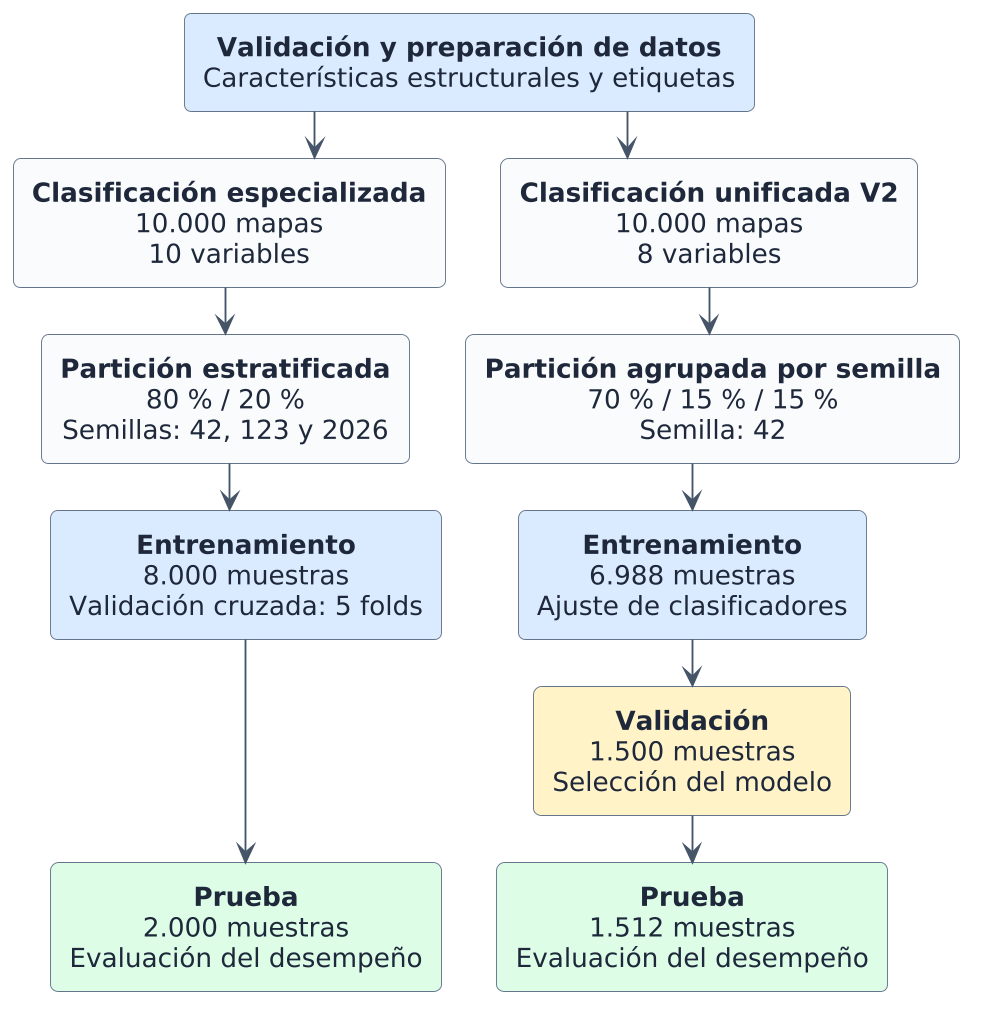
\includegraphics[
	width=0.95\textwidth,
	height=0.70\textheight,
	keepaspectratio
	]{imagenes/particion_datasets_experimentales.png}
	
	\caption{Comparación de las estrategias de partición de los conjuntos de datos experimentales de Rhyzome}
	
	\label{fig:particion_datasets_experimentales}
	
\end{figure}

\FloatBarrier

Como se observa en la figura, el experimento de clasificación especializada utiliza validación cruzada interna sobre el conjunto de entrenamiento, mientras que el experimento de clasificación unificada establece un conjunto de validación independiente y realiza la separación de las muestras considerando las semillas de generación.

\textbf{Prevención de fuga de información.}

La fuga de información puede producirse cuando datos o propiedades correspondientes a las muestras de evaluación intervienen en el entrenamiento de los clasificadores, generando estimaciones de desempeño que no representan adecuadamente su comportamiento ante datos no utilizados durante el aprendizaje.

En ambos procedimientos experimentales se reduce el riesgo de fuga asociado a la estandarización mediante la incorporación de las transformaciones dentro de los pipelines de entrenamiento. Asimismo, las variables auxiliares correspondientes al índice estructural y a la complejidad observada no forman parte de las variables de entrada utilizadas por los clasificadores.

En el experimento de clasificación unificada se incorpora adicionalmente un control explícito sobre la separación de las semillas. Sean $\mathcal{S}_{\mathrm{ent}}$, $\mathcal{S}_{\mathrm{val}}$ y $\mathcal{S}_{\mathrm{pru}}$ los conjuntos de semillas correspondientes a entrenamiento, validación y prueba, respectivamente. El procedimiento verifica el cumplimiento de las siguientes condiciones:

\begin{equation}
	\begin{aligned}
		\mathcal{S}_{\mathrm{ent}}
		\cap
		\mathcal{S}_{\mathrm{val}}
		&= \varnothing,\\
		\mathcal{S}_{\mathrm{ent}}
		\cap
		\mathcal{S}_{\mathrm{pru}}
		&= \varnothing,\\
		\mathcal{S}_{\mathrm{val}}
		\cap
		\mathcal{S}_{\mathrm{pru}}
		&= \varnothing.
	\end{aligned}
	\label{eq:separacion_semillas}
\end{equation}

Ante el incumplimiento de alguna de estas condiciones, el procedimiento interrumpe la ejecución del entrenamiento. Este control garantiza que los registros asociados a una misma semilla no se distribuyan entre diferentes particiones del conjunto de datos.

Por su parte, el experimento de clasificación especializada utiliza una separación estratificada por muestras, sin incorporar un mecanismo explícito de agrupación o verificación de intersección de semillas. Esta diferencia constituye una consideración metodológica relevante al interpretar y comparar los resultados de ambos procedimientos.

En consecuencia, las estrategias adoptadas permiten controlar fuentes específicas de fuga de información relacionadas con el escalado y la separación de las muestras. Sin embargo, estos controles no constituyen una garantía absoluta de independencia estructural entre todos los mapas, puesto que diferentes semillas pueden producir escenarios con características similares o incluso estructuras equivalentes.


% ============================================================
\section{Entrenamiento: algoritmos y parámetros}
\label{sec:entrenamiento_ia}

El entrenamiento del componente de aprendizaje automático de Rhyzome se realiza mediante un procedimiento experimental independiente del entorno de producción, orientado a identificar clasificadores capaces de reconocer los perfiles de complejidad de los mapas generados proceduralmente.

Esta sección describe el diseño de la experimentación, los algoritmos evaluados, la configuración de sus hiperparámetros y las condiciones establecidas para favorecer la reproducibilidad del proceso de entrenamiento.

\subsection{Diseño de la experimentación}
\label{subsec:diseno_experimentacion}

El diseño experimental se fundamenta en la comparación de algoritmos de aprendizaje supervisado bajo condiciones controladas de generación, preparación y evaluación de los datos. Su finalidad consiste en identificar configuraciones de clasificación adecuadas para las características estructurales de los escenarios contemplados por Rhyzome, considerando tanto el desempeño predictivo como las condiciones necesarias para su posterior integración con la aplicación.

El entrenamiento se realiza fuera del entorno de producción, permitiendo evaluar diferentes alternativas de clasificación sin afectar la disponibilidad de los servicios de generación procedural. Los modelos seleccionados se exportan como artefactos reutilizables, de manera que la aplicación pueda ejecutar las
predicciones sin realizar nuevamente el proceso de entrenamiento.

\textbf{Objetivo experimental.}

El objetivo de la experimentación consiste en evaluar la capacidad de diferentes algoritmos de aprendizaje supervisado para identificar los perfiles de complejidad baja, media y alta a partir de las características estructurales de los mapas.

Para ello, se consideran los seis clasificadores descritos en la sección correspondiente al tipo de modelo utilizado: Regresión Logística, K-Nearest Neighbors (KNN), Random Forest, Support Vector Machine (SVM), Gradient Boosting y Multilayer Perceptron (MLP).

La selección de estos algoritmos permite comparar diferentes enfoques de aprendizaje, incluyendo modelos lineales, métodos basados en distancias, conjuntos de árboles de decisión, clasificadores basados en márgenes y redes neuronales artificiales \parencite{james2023}.

La experimentación busca determinar qué alternativas presentan un desempeño adecuado dentro de las condiciones establecidas para Rhyzome, sin asumir previamente que un algoritmo particular constituye la mejor solución para todos los escenarios.

\textbf{Estrategias experimentales.}

Se consideran dos estrategias de clasificación, denominadas experimento de clasificación especializada (E1) y experimento de clasificación unificada (E2). Cada estrategia dispone de un conjunto de datos independiente, cuya composición y preparación se describen en las subsecciones anteriores.

El experimento de clasificación especializada considera inicialmente una evaluación global de los seis clasificadores sobre el conjunto completo de mapas. Posteriormente, se realiza una evaluación independiente para las familias procedurales de Perlin Noise y Autómatas Celulares, con el propósito
de determinar si las particularidades estructurales de cada familia favorecen la selección de clasificadores diferentes.

Por su parte, el experimento de clasificación unificada evalúa los seis algoritmos sobre un conjunto de datos que incorpora los cuatro biomas de Rhyzome V2. Este enfoque busca identificar un único clasificador capaz de reconocer los perfiles de complejidad independientemente del bioma y del
mecanismo generativo utilizado para construir el escenario.

La Tabla~\ref{tab:estrategias_experimentales_ml} resume las principales diferencias entre los dos procedimientos experimentales.

\begin{table}[htbp]
	\centering
	
	\caption{Comparación de las estrategias experimentales de clasificación en Rhyzome}
	
	\label{tab:estrategias_experimentales_ml}
	
	\renewcommand{\arraystretch}{1.5}
	
	\begin{tabularx}{\textwidth}{
			|>{\raggedright\arraybackslash}p{3.2cm}|
			>{\raggedright\arraybackslash}X|
			>{\raggedright\arraybackslash}X|
		}
		
		\hline
		
		\rowcolor{gray!15}
		\textbf{Característica} &
		\textbf{Clasificación especializada (E1)} &
		\textbf{Clasificación unificada (E2)}
		\\ \hline
		
		Objetivo &
		Seleccionar un clasificador por familia
		procedural. &
		Seleccionar un clasificador común para
		los cuatro biomas. \\ \hline
		
		Clasificadores evaluados &
		Seis. &
		Seis. \\ \hline
		
		Variables de entrada &
		Diez características. &
		Ocho características estructurales.
		\\ \hline
		
		Estrategia de partición &
		Estratificada 80/20. &
		Agrupada por semilla 70/15/15.
		\\ \hline
		
		Semillas experimentales &
		42, 123 y 2026. &
		42. \\ \hline
		
		Validación &
		Validación cruzada estratificada
		de cinco particiones. &
		Conjunto de validación independiente.
		\\ \hline
		
		Criterio principal de selección &
		F1 macro promedio de validación cruzada. &
		F1 macro del conjunto de validación.
		\\ \hline
		
		Criterios secundarios de selección &
		ROC-AUC multiclase y tiempo de inferencia. &
		No establecidos explícitamente.
		\\ \hline
		
		Artefactos seleccionados &
		Dos clasificadores especializados. &
		Un clasificador unificado.
		\\ \hline
		
	\end{tabularx}
	
\end{table}

\FloatBarrier

Ambas estrategias comparten el objetivo de reconocer los perfiles generativos de complejidad. Sin embargo, difieren en las condiciones de construcción de los datos, las características utilizadas y los procedimientos de validación. Por esta razón, cada estrategia se analiza dentro de su propio contexto
experimental.

\textbf{Variables y condiciones experimentales.}

La comparación de los clasificadores requiere establecer las variables que intervienen en el procedimiento experimental y las condiciones que se mantienen constantes durante su ejecución.

La principal variable independiente corresponde al algoritmo de clasificación evaluado, junto con la configuración de hiperparámetros asociada a cada estimador. En el experimento especializado también se considera la familia procedural como factor de agrupación de las muestras.

Las variables dependientes corresponden a las métricas obtenidas durante la evaluación de los clasificadores. Estas permiten cuantificar su capacidad para reconocer las categorías de complejidad y, cuando corresponde, analizar los tiempos asociados al entrenamiento y la inferencia.

La Tabla~\ref{tab:variables_experimentales_ml} presenta las principales variables y condiciones consideradas durante la experimentación.

\begin{table}[htbp]
	\centering
	
	\caption{Variables y condiciones del diseño	experimental de clasificación}
	
	\label{tab:variables_experimentales_ml}
	
	\renewcommand{\arraystretch}{1.5}
	
	\begin{tabularx}{\textwidth}{
			|>{\raggedright\arraybackslash}p{3.2cm}|
			>{\raggedright\arraybackslash}X|
		}
		
		\hline
		
		\rowcolor{gray!15}
		\textbf{Tipo} &
		\textbf{Descripción} \\ \hline
		
		Variable independiente &
		Algoritmo de clasificación y configuración
		de hiperparámetros asociada. \\ \hline
		
		Factor de agrupación &
		Familia procedural en E1 y conjunto
		unificado de biomas en E2. \\ \hline
		
		Variables dependientes &
		Métricas de clasificación y, en E1,
		tiempos de entrenamiento e inferencia.
		\\ \hline
		
		Variable objetivo &
		Perfil de complejidad solicitado:
		bajo, medio o alto. \\ \hline
		
		Condiciones controladas &
		Conjunto de datos, características de
		entrada, codificación de etiquetas y
		estrategia de partición dentro de cada
		procedimiento experimental. \\ \hline
		
		Control de aleatoriedad &
		Semillas establecidas para la generación,
		partición y entrenamiento de los modelos,
		según la configuración experimental.
		\\ \hline
		
	\end{tabularx}
	
\end{table}

\FloatBarrier

Dentro de cada procedimiento experimental, los clasificadores se evalúan utilizando las mismas particiones de datos y la misma representación de las características. Las transformaciones requeridas por cada algoritmo se incorporan mediante los mecanismos de preprocesamiento descritos en la Subsección~\ref{subsec:preprocesamiento_dataset}.

Esta configuración permite reducir la influencia de diferencias ajenas al algoritmo evaluado, aunque los resultados también dependen de los hiperparámetros establecidos para cada estimador.

\textbf{Protocolo de experimentación.}

El protocolo experimental comprende la preparación de los conjuntos de datos, la configuración de los clasificadores, el entrenamiento, la evaluación del desempeño y la selección de los artefactos destinados a la integración con Rhyzome.

La Figura~\ref{fig:estrategias_clasificacion_experimental} presenta el flujo de experimentación correspondiente a las estrategias de clasificación especializada y unificada.

\begin{figure}[htbp]
	\centering
	
	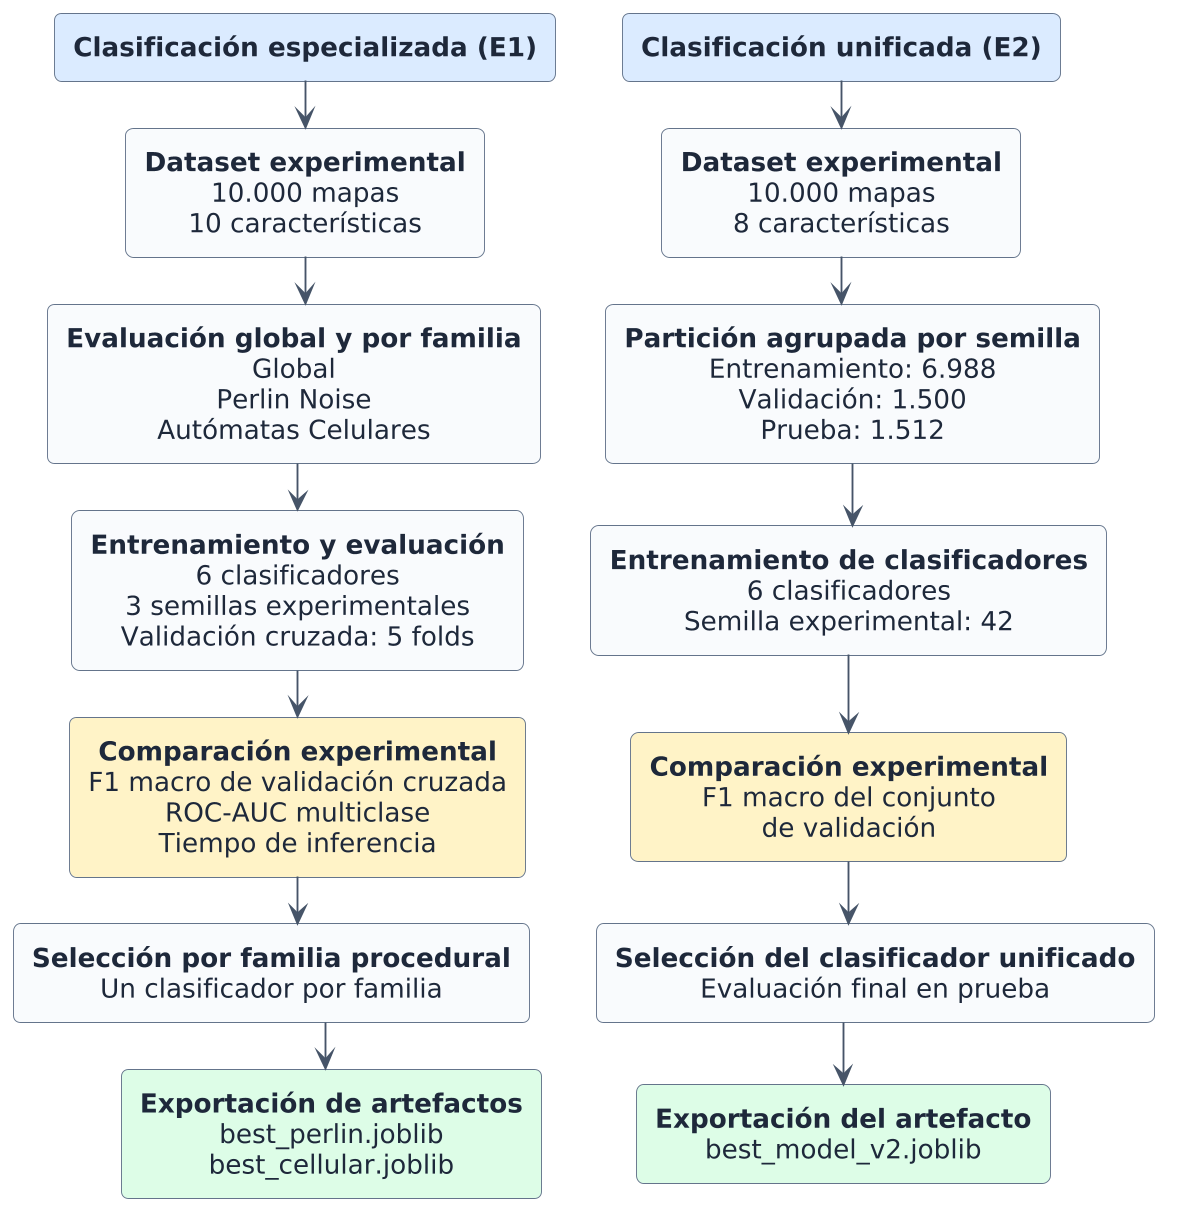
\includegraphics[
	width=0.95\textwidth,
	height=0.75\textheight,
	keepaspectratio
	]{imagenes/estrategias_clasificacion_experimental.png}
	
	\caption{Diseño de las estrategias experimentales de clasificación de complejidad en Rhyzome}
	
	\label{fig:estrategias_clasificacion_experimental}
	
\end{figure}

\FloatBarrier

Como se observa en la figura, ambos procedimientos parten de conjuntos de datos previamente preparados y etiquetados. La estrategia especializada realiza una evaluación global y posteriormente una comparación independiente por familia procedural, mientras que la estrategia unificada utiliza un conjunto común de muestras y una separación agrupada por semilla.

En el experimento especializado, cada clasificador se evalúa mediante validación cruzada estratificada de cinco particiones, utilizando las semillas experimentales 42, 123 y 2026. Para cada semilla, el estimador también se ajusta sobre el conjunto completo de entrenamiento y se evalúa utilizando el conjunto de prueba correspondiente.

Considerando los seis clasificadores, las tres semillas y las cinco particiones de validación cruzada, el número de ajustes por cada ámbito de evaluación se determina mediante:

\begin{equation}
	N_{\mathrm{CV}} =
	N_{\mathrm{modelos}}
	\times
	N_{\mathrm{semillas}}
	\times
	N_{\mathrm{folds}}
	\label{eq:ajustes_validacion_experimental}
\end{equation}

Al sustituir los valores establecidos en el protocolo experimental, se obtiene:

\begin{equation}
	N_{\mathrm{CV}} = 6 \times 3 \times 5 = 90
	\label{eq:ajustes_cv_por_ambito}
\end{equation}

La evaluación global y las evaluaciones independientes de Perlin Noise y Autómatas Celulares representan tres ámbitos de experimentación. Por consiguiente, el protocolo comprende 270 ajustes de estimadores durante la validación cruzada, además de 54 ajustes sobre los respectivos conjuntos completos de entrenamiento para la evaluación en prueba.

La Tabla~\ref{tab:ajustes_experimentales_ml} resume la cantidad de ajustes principales correspondientes al experimento especializado.

\begin{table}[htbp]
	\centering
	
	\caption{Cantidad de ajustes de estimadores	en el experimento de clasificación especializada}
	
	\label{tab:ajustes_experimentales_ml}
	
	\renewcommand{\arraystretch}{1.5}
	
	\begin{tabularx}{\textwidth}{
			|>{\raggedright\arraybackslash}X|
			>{\centering\arraybackslash}p{2.3cm}|
			>{\centering\arraybackslash}p{2.5cm}|
			>{\centering\arraybackslash}p{1.7cm}|
		}
		
		\hline
		
		\rowcolor{gray!15}
		\textbf{Ámbito de evaluación} &
		\textbf{Ajustes CV} &
		\textbf{Ajustes para prueba} &
		\textbf{Total} \\ \hline
		
		Evaluación global &
		90 & 18 & 108 \\ \hline
		
		Perlin Noise &
		90 & 18 & 108 \\ \hline
		
		Autómatas Celulares &
		90 & 18 & 108 \\ \hline
		
		\rowcolor{gray!10}
		\textbf{Total} &
		\textbf{270} &
		\textbf{54} &
		\textbf{324} \\ \hline
		
	\end{tabularx}
	
\end{table}

\FloatBarrier

Los valores presentados corresponden a los ajustes principales establecidos por los ciclos de experimentación y no incluyen posibles operaciones internas de entrenamiento realizadas por los estimadores ni ajustes adicionales asociados a la exportación de artefactos.

En el experimento de clasificación unificada, los seis clasificadores se ajustan utilizando el conjunto de entrenamiento y se comparan mediante sus resultados sobre el conjunto de validación. Una vez seleccionado el estimador con mejor desempeño según el criterio establecido, se realiza su evaluación sobre el conjunto de prueba.

\textbf{Criterios de selección de los clasificadores.}

El criterio principal de selección en ambos procedimientos experimentales corresponde a la métrica F1 macro, debido a que permite considerar conjuntamente la precisión y la exhaustividad de las predicciones, otorgando la misma importancia a cada categoría de complejidad.

En el experimento especializado, el criterio principal se obtiene mediante el promedio de los valores de F1 macro registrados durante la validación cruzada para las tres semillas experimentales.

Sea $F_{s,k}(m,g)$ el valor de F1 macro obtenido por el clasificador $m$, correspondiente a la familia procedural $g$, la semilla experimental $s$ y la partición de validación cruzada $k$. El desempeño promedio se expresa mediante:

\begin{equation}
	\overline{F}_{\mathrm{CV}}(m,g)
	=
	\frac{1}{15}
	\sum_{s=1}^{3}
	\sum_{k=1}^{5}
	F_{s,k}(m,g)
	\label{eq:f1_promedio_experimental}
\end{equation}

La selección se realiza de manera independiente para cada familia procedural, ordenando los clasificadores según los siguientes criterios:

\begin{enumerate}
	\item Mayor F1 macro promedio de validación cruzada.
	
	\item Mayor ROC-AUC multiclase macro, mediante la estrategia One-vs-Rest, cuando existe igualdad en el criterio principal.
	
	\item Menor tiempo promedio de inferencia por mapa, cuando existe igualdad en los criterios anteriores.
\end{enumerate}

Los criterios se aplican de manera jerárquica, sin combinar las métricas mediante ponderaciones o una función de puntuación adicional.

En este procedimiento, el ROC-AUC y el tiempo de inferencia utilizados como criterios secundarios se obtienen a partir de las evaluaciones sobre los conjuntos de prueba. Por consiguiente, estas muestras no constituyen una evaluación completamente independiente del procedimiento de selección cuando intervienen dichos criterios secundarios.

En el experimento unificado, la selección se realiza exclusivamente mediante el F1 macro obtenido sobre el conjunto de validación. Sea $\mathcal{M}$ el conjunto de clasificadores evaluados. El modelo seleccionado se expresa mediante:

\begin{equation}
	m_{\mathrm{uni}}^{*}
	=
	\operatorname*{arg\,max}_{m \in \mathcal{M}}
	F_{1,\mathrm{macro}}^{\mathrm{val}}(m)
	\label{eq:seleccion_modelo_unificado}
\end{equation}

El clasificador seleccionado se evalúa posteriormente sobre el conjunto de prueba, manteniendo una separación entre las muestras utilizadas para el ajuste, la selección y la evaluación final.

La definición formal de las métricas utilizadas durante ambos procedimientos se desarrolla en la sección correspondiente a las métricas de evaluación, mientras que los resultados y la justificación de los modelos seleccionados se presentan en la sección de desempeño experimental.

\textbf{Alcance de la comparación experimental.}

El diseño adoptado permite comparar los clasificadores bajo condiciones comunes dentro de cada estrategia experimental. No obstante, los resultados de la clasificación especializada y la clasificación unificada deben interpretarse considerando las diferencias existentes entre sus conjuntos de datos, mecanismos generativos, características de entrada y procedimientos de validación.

Por consiguiente, las diferencias de desempeño entre ambos experimentos no pueden atribuirse exclusivamente al algoritmo de clasificación o a la exclusión de las dimensiones del mapa como variables de entrada.

Asimismo, los resultados experimentales representan la capacidad de los modelos para reconocer los perfiles generativos de complejidad definidos en Rhyzome, y no una medición independiente de la dificultad percibida por los jugadores.


\subsection{Entrenamiento y comparación de modelos por familia}
% Explicar ejecución paso a paso: carga, extracción, etiquetas, partición, entrenamiento y evaluación.
% Confirmar si se entrenaron modelos independientes por familia y cómo se compararon.
% Los resultados numéricos se presentan en la Sección 4.6, no duplicarlos aquí.
Se construyen los vectores de entrada, se codifica la complejidad solicitada y se realizan comparaciones globales y por familia. Para cada semilla se ajustan los clasificadores y se evalúan sobre la partición de prueba. Los artefactos seleccionados por familia se exportan con semilla 42. \pendiente{Confirmar la denominación histórica de las etapas con evidencias distintas de las dos copias idénticas del notebook.}

\subsection{Configuración de hiperparámetros}
% Distinguir hiperparámetros fijos, búsqueda de hiperparámetros y parámetros aprendidos.
% No afirmar GridSearchCV ni optimización si no aparecen en el notebook.
\begin{table}[htbp]
	\centering
	\caption{Configuración de los clasificadores evaluados}
	\label{tab:hiperparametros_ia}
	\renewcommand{\arraystretch}{1.5}
	\begin{tabularx}{\textwidth}{|>{\raggedright\arraybackslash}p{3.5cm}|X|X|}
		\hline
		\rowcolor{gray!15} \textbf{Modelo} & \textbf{Hiperparámetros} & \textbf{Valores utilizados} \\ \hline
		Regresión Logística & Iteraciones máximas; pesos & 2000; balanceados \\ \hline
		KNN & Vecinos; pesos & 7; distancia \\ \hline
		Random Forest & Árboles; pesos & 300; balanceados \\ \hline
		SVM (RBF) & C; probabilidades; pesos & 2; activadas; balanceados \\ \hline
		Gradient Boosting & Estimadores; tasa; profundidad & 150; 0,05; 3 \\ \hline
		MLP & Capas; iteraciones; parada temprana & 64 y 32; 1000; activada \\ \hline
	\end{tabularx}
\end{table}
\FloatBarrier
La tabla corresponde al constructor de modelos del notebook de 10.000 mapas. % Verificar por separado hiperparámetros V2.

\subsection{Reproducibilidad del entrenamiento}
% Registrar Python, scikit-learn, NumPy, semillas, notebook, versión del dataset y commit si existe.
% Diferenciar versiones del entorno experimental de las del backend.
El manifiesto registra Python 3.13.15, scikit-learn 1.6.1, Joblib 1.6.0, NumPy 2.1.3 y pandas 2.2.3. Incluye hashes SHA-256 de los dos artefactos especializados. \pendiente{Confirmar versiones efectivas del despliegue y compatibilidad de serialización.}

% ============================================================
\section{Métricas de evaluación}
\label{sec:metricas_ia}

\subsection{Métricas de clasificación}
% Conservar únicamente las métricas efectivamente utilizadas; agregar referencias bibliográficas.
La evaluación de un clasificador multiclase puede realizarse mediante exactitud, precisión, sensibilidad y puntuación F1. Para una clase determinada, $VP$, $FP$ y $FN$ representan verdaderos positivos, falsos positivos y falsos negativos, respectivamente.
\begin{equation}
	\mathrm{Accuracy}=\frac{\sum_{i=1}^{N}\mathbf{1}(y_i=\hat{y}_i)}{N}
\end{equation}
\begin{equation}
	P=\frac{VP}{VP+FP},\qquad R=\frac{VP}{VP+FN}
\end{equation}
\begin{equation}
	F_1=\frac{2PR}{P+R},\qquad F_{1,\mathrm{macro}}=\frac{1}{K}\sum_{k=1}^{K}F_{1,k}
\end{equation}
Aquí $N$ representa el número de muestras evaluadas y $K$ el número de clases. El promedio macro asigna el mismo peso a cada clase.
% Confirmar tratamiento de denominadores cero y tipo de promedio realmente usado.
Además de estas métricas se reportan exactitud balanceada y ROC-AUC multiclase One-vs-Rest. El criterio principal del estudio por familia es F1 macro de validación cruzada.

\subsection{Matrices de confusión}
% Incorporar matrices reales, preferiblemente de los modelos seleccionados por familia.
% Indicar partición, orden de clases, ejes real/predicho y si son conteos o porcentajes.
% Analizar confusiones entre clases, no limitarse a insertar imágenes.
Para V2, la matriz de prueba registrada, con filas reales y columnas predichas en orden bajo, medio y alto, es:\begin{equation}\begin{pmatrix}493&11&0\\9&490&5\\0&4&500\end{pmatrix}\end{equation} Se observan 29 errores en 1.512 muestras, principalmente entre clases adyacentes. \pendiente{Incorporar matrices de los clasificadores especializados.}

\subsection{Métricas estructurales de los mapas}
Las métricas estructurales describen propiedades de los escenarios y se distinguen de las métricas de desempeño de clasificación.
% Confirmar conectividad, accesibilidad, densidad de obstáculos y demás indicadores implementados.
% Explicar su función en la evaluación adaptativa y diferenciar métricas de entrada y salida.
\pendiente{Documentar las métricas estructurales utilizadas y sus definiciones verificadas.}

% ============================================================
\section{Validación cruzada}
\label{sec:validacion_cruzada_ia}
\subsection{Estrategia de validación experimental}
% Verificar si hubo K-fold, StratifiedKFold, holdout u otro procedimiento.
% Si no hubo validación cruzada, declararlo expresamente; no presentar holdout como K-fold.
% Si existe K-fold, registrar k, semillas, media, desviación estándar y separación por grupos si aplica.
El estudio por familia utiliza Stratified K-Fold con cinco particiones, barajado y semillas 42, 123 y 2026. El registro V2 presenta una partición de validación independiente; no debe describirse como validación cruzada sin evidencia adicional.

\subsection{Evaluación con mapas externos}
La comparación con las 200 ventanas externas de Zelda descritas en la Sección~\ref{subsec:origen_dataset} examina las distribuciones de características estructurales. No constituye validación cruzada ni una medición de exactitud externa.
% Identificar fuentes, licencias, conversión a matrices, etiquetas y resultados.
% Confirmar que los mapas de evaluación no participaron en el entrenamiento.
% Si no existen etiquetas independientes, no presentar coincidencias como exactitud externa.
\pendiente{Incorporar los resultados de la comparación de distribuciones externas registrados en el notebook.}

\subsection{Limitaciones de la generalización}
% Analizar diferencias de dominio, dimensiones, distribución de clases, duplicados y criterio de etiquetado.
% Distinguir limitaciones observadas de riesgos metodológicos potenciales.
\pendiente{Discutir las limitaciones respaldadas por los resultados experimentales.}

% ============================================================
\section{Desempeño y justificación de selección}
\label{sec:desempeno_ia}
\subsection{Resultados de los modelos para Perlin Noise}
% FUENTE: salidas del notebook y manifiesto; usar la misma partición y métricas comparables.
\begin{table}[htbp]
	\centering
	\caption{Resultados de clasificación para Perlin Noise}
	\label{tab:resultados_perlin}
	\renewcommand{\arraystretch}{1.5}
	\begin{tabularx}{\textwidth}{|X|c|c|c|c|}
		\hline
		\rowcolor{gray!15} \textbf{Modelo} & \textbf{Accuracy} & \textbf{Precisión} & \textbf{Recall} & \textbf{F1} \\ \hline
		Regresión Logística & 0,8218 & 0,8216 & 0,8218 & 0,8207 \\ \hline
		SVM (RBF) & 0,8116 & 0,8097 & 0,8116 & 0,8091 \\ \hline
		Gradient Boosting & 0,8087 & 0,8070 & 0,8087 & 0,8071 \\ \hline
		Random Forest & 0,8064 & 0,8047 & 0,8064 & 0,8050 \\ \hline
		MLP & 0,8022 & 0,8009 & 0,8022 & 0,8006 \\ \hline
		KNN & 0,7409 & 0,7389 & 0,7409 & 0,7391 \\ \hline
	\end{tabularx}
\end{table}
\FloatBarrier
% Ajustar columnas al promedio y métricas reales. Agregar gráfica comparativa si aporta información.
Los valores de la tabla corresponden a métricas de prueba agregadas, no a la validación cruzada. El criterio de selección se presenta en la subsección de selección de modelos.

\subsection{Resultados de los modelos para Autómatas Celulares}
\begin{table}[htbp]
	\centering
	\caption{Resultados de clasificación para Autómatas Celulares}
	\label{tab:resultados_cellular}
	\renewcommand{\arraystretch}{1.5}
	\begin{tabularx}{\textwidth}{|X|c|c|c|c|}
		\hline
		\rowcolor{gray!15} \textbf{Modelo} & \textbf{Accuracy} & \textbf{Precisión} & \textbf{Recall} & \textbf{F1} \\ \hline
		MLP & 0,8293 & 0,8360 & 0,8293 & 0,8304 \\ \hline
		Random Forest & 0,8007 & 0,8088 & 0,8006 & 0,8020 \\ \hline
		Gradient Boosting & 0,7860 & 0,7981 & 0,7860 & 0,7881 \\ \hline
		SVM (RBF) & 0,8033 & 0,8372 & 0,8035 & 0,8058 \\ \hline
		KNN & 0,7673 & 0,7941 & 0,7674 & 0,7692 \\ \hline
		Regresión Logística & 0,7067 & 0,7270 & 0,7068 & 0,7048 \\ \hline
	\end{tabularx}
\end{table}
\FloatBarrier
Los valores de la tabla corresponden a métricas de prueba agregadas, no a la validación cruzada.

\subsection{Selección de los modelos definitivos}
% Contrastar winners del manifiesto con artefactos desplegados y criterio real de selección.
% No atribuir la selección a velocidad o tamaño si no se midieron.
El manifiesto selecciona Regresión Logística para Perlin Noise y MLP para Autómatas Celulares, con F1 macro de validación cruzada de 0,8203 y 0,8054, respectivamente. Los artefactos exportados son \texttt{best\_perlin.joblib} y \texttt{best\_cellular.joblib}.

\subsection{Resultados del entrenamiento V2}
El registro \texttt{training\_results.json} documenta un entrenamiento adicional con ocho características y un clasificador único. La Tabla~\ref{tab:resultados_v2} presenta el F1 macro de validación.
\begin{table}[htbp]
	\centering
	\caption{Comparación de clasificadores V2}
	\label{tab:resultados_v2}
	\renewcommand{\arraystretch}{1.5}
	\begin{tabularx}{\textwidth}{|X|c|}\hline
		\rowcolor{gray!15} \textbf{Modelo} & \textbf{F1 macro} \\ \hline
		Logistic Regression & 0,8775 \\ \hline
		Knn & 0,9813 \\ \hline
		Random Forest & 0,9840 \\ \hline
		Svm & 0,9767 \\ \hline
		Gradient Boosting & 0,9780 \\ \hline
		Mlp & 0,9780 \\ \hline
	\end{tabularx}
\end{table}
\FloatBarrier
Random Forest fue seleccionado con F1 macro de validación de 0,9840 y obtuvo exactitud y F1 macro de 0,9808 en prueba. Estos resultados no constituyen una comparación controlada con el estudio por familia, debido a las diferencias en características y particiones.

\subsection{Evaluación de la generación adaptativa}
Esta etapa utiliza modelos previamente entrenados para evaluar su participación en la generación y selección de mapas candidatos. No corresponde a un nuevo entrenamiento de los clasificadores.
% FUENTE: notebook o registros de la evaluación adaptativa, respuestas JSON y mapas generados.
% Describir objetivo, escenarios, semillas, dimensiones, clases solicitadas e intentos.
% Confirmar criterio de selección y significado de target_probability; no confundir probabilidad con exactitud.
% Si se midió tasa de coincidencia, definir denominador y aclarar que es coincidencia predicha, no verdad independiente.
% Incorporar ejemplos de mapas, resultados por familia y clase, y comparación base/adaptativa solo si se ejecutó.
\begin{table}[htbp]
	\centering
	\caption{Resultados de la evaluación de generación adaptativa}
	\label{tab:resultados_adaptativos}
	\renewcommand{\arraystretch}{1.5}
	\begin{tabularx}{\textwidth}{|X|X|c|c|}
		\hline
		\rowcolor{gray!15} \textbf{Familia} & \textbf{Clase objetivo} & \textbf{Solicitudes} & \textbf{Coincidencias} \\ \hline
		Por confirmar & Por confirmar & -- & -- \\ \hline
	\end{tabularx}
\end{table}
\FloatBarrier
\pendiente{Completar el protocolo, las evidencias y los resultados reales del protocolo de evaluación adaptativa.}

\subsection{Análisis y discusión de resultados}
% Interpretar ambos experimentos: desempeño predictivo frente a utilidad en generación adaptativa.
% Relacionar resultados con objetivos específicos y limitaciones; no repetir tablas completas.
% Las pruebas funcionales, API y rendimiento del sistema corresponden al capítulo 6.
\pendiente{Redactar la discusión a partir de los resultados consolidados.}

% ============================================================
\section{Integración con la aplicación}
\label{sec:integracion_aplicacion_ia}
\subsection{Artefactos resultantes del entrenamiento}
Los modelos seleccionados se incorporan al backend mediante artefactos serializados. La estrategia arquitectónica de integración se describe en la Sección~\ref{sec:integracion_ia}.
% Verificar nombres, versiones y correspondencia entre manifiesto y modelos desplegados.
% Referenciar la tabla del capítulo 3 en lugar de duplicarla, tras confirmar su etiqueta.
El repositorio contiene los artefactos especializados y el adaptador V2 que carga un modelo único. Se deben mantener separados sus contratos de características y clases. \pendiente{Confirmar cuál corresponde al despliegue definitivo y ajustar la sección 3.5 si procede.}

\subsection{Proceso de inferencia en producción}
% FUENTE: ml_adapter.py, generador adaptativo y configuración de características.
% Explicar orden de entradas, transformación, predicción, clases y probabilidades según implementación.
% No repetir el diagrama de secuencia ni la formalización de selección del capítulo 3.
El servicio adaptativo V2 ejecuta todos los intentos configurados (entre 1 y 50), utilizando semillas consecutivas. Prioriza candidatos cuya clase predicha coincide con la solicitada y luego maximiza la probabilidad de dicha clase. En caso de empate exacto conserva el primer candidato. No reentrena el clasificador. \pendiente{Confirmar ruta y modelo activos en producción.}

\subsection{Trazabilidad y reproducibilidad}
% Relacionar notebook -> dataset -> resultados -> manifiesto -> artefacto -> backend.
% Incorporar identificadores de versión, semillas y evidencias disponibles; remitir pruebas al capítulo 6.
\pendiente{Consolidar la trazabilidad experimental y de despliegue.}

% ============================================================
\section{Consideraciones éticas y sesgo algorítmico}
\label{sec:etica_ia}
\subsection{Sesgos asociados al dataset y etiquetado}
La representatividad de las muestras depende de la cobertura de configuraciones procedurales y del criterio de etiquetado.
% Relacionar estos riesgos con los conteos y reglas reales; no afirmar sesgos medidos sin evidencia.
Las etiquetas representan perfiles generativos solicitados y no juicios independientes de jugadores. Por tanto, un alto desempeño predictivo indica capacidad de recuperar esos perfiles, no una validación de dificultad jugable. La distribución por familia también limita la interpretación de resultados globales.

\subsection{Limitaciones del modelo de complejidad}
La complejidad estimada corresponde a propiedades estructurales de los mapas. No constituye por sí sola una garantía de jugabilidad, dificultad percibida, calidad narrativa o experiencia satisfactoria para el jugador.
% Explicar límites de dominio, dependencia de etiquetas y ausencia de validación con jugadores si corresponde.
\pendiente{Precisar las limitaciones observadas y el alcance de las conclusiones.}

\subsection{Licenciamiento y uso responsable}
% Registrar licencia de cada fuente externa, condiciones de reutilización y atribución.
% Distinguir uso académico de autorización para redistribuir mapas o recursos de videojuegos.
% No afirmar ausencia de datos personales ni permisos sin comprobar las fuentes.
La procedencia de los niveles externos y las limitaciones de trazabilidad se describen en la Sección~\ref{subsec:origen_dataset}. El uso académico no implica por sí mismo autorización para redistribuir recursos de los videojuegos originales. \pendiente{Verificar las condiciones de licencia aplicables a los archivos externos utilizados.}

\FloatBarrier
% CONTROL FINAL: eliminar marcadores pendientes, verificar referencias y citas,
% reemplazar todas las filas provisionales, compilar y revisar tablas y figuras.
% Confirmar que las conclusiones coinciden con los notebooks y el backend definitivo.


% Capítulo 5: Gestión Ágil del Proyecto (SCRUM)
\chapter{Gestión Ágil del Proyecto (SCRUM)}
\label{cap:05_gestion_agil}

\section{Backlog del producto}
\pendiente{Desarrollar este apartado con metodología, resultados, decisiones y evidencias verificables.}

\section{Historias de usuario, criterios de aceptación y DoD}
\pendiente{Desarrollar este apartado con metodología, resultados, decisiones y evidencias verificables.}

\section{Planificación de sprints}
\pendiente{Desarrollar este apartado con metodología, resultados, decisiones y evidencias verificables.}

\section{Velocidad por sprint}
\pendiente{Desarrollar este apartado con metodología, resultados, decisiones y evidencias verificables.}

\section{Burndown charts}
\pendiente{Desarrollar este apartado con metodología, resultados, decisiones y evidencias verificables.}

\section{Evidencias de dailies, retrospectivas y revisiones}
\pendiente{Desarrollar este apartado con metodología, resultados, decisiones y evidencias verificables.}

\section{Responsabilidades y colaboración del equipo}
\pendiente{Desarrollar este apartado con metodología, resultados, decisiones y evidencias verificables.}


% Capítulo 6: Pruebas y Validación del Sistema
\chapter{Pruebas y Validación del Sistema}
\label{cap:06_pruebas_validacion}

\section{Plan de pruebas}
\pendiente{Desarrollar este apartado con metodología, resultados, decisiones y evidencias verificables.}

\section{Cobertura de pruebas}
\pendiente{Desarrollar este apartado con metodología, resultados, decisiones y evidencias verificables.}

\section{Matriz de trazabilidad entre requisitos y pruebas}
\pendiente{Desarrollar este apartado con metodología, resultados, decisiones y evidencias verificables.}

\begin{table}[htbp]\centering
\caption{Matriz de trazabilidad (ejemplo editable)}\label{tab:trazabilidad}
\begin{tabularx}{\textwidth}{@{}lXll@{}}\toprule
Requisito & Caso de prueba & Resultado & Evidencia \\\midrule
HU-XX & TC-XX: descripción & Pendiente & EV-XX \\\bottomrule
\end{tabularx}\end{table}

\section{Resultados de las pruebas}

\begin{table}[htbp]
    \centering

    \caption{Matriz de verificación de la integración del componente inteligente}
    \label{tab:resultados_integracion_ia}

    \renewcommand{\arraystretch}{1.2}

    \begin{tabularx}{\textwidth}{
        |>{\raggedright\arraybackslash}p{3cm}|
         >{\raggedright\arraybackslash}X|
         >{\raggedright\arraybackslash}X|
    }
        \hline

        \rowcolor{gray!15}
        \textbf{Componente} &
        \textbf{Comportamiento esperado} &
        \textbf{Evidencia por vincular} \\

        \hline

        \textbf{Configuración de complejidad} &
        Selección del nivel de complejidad requerido
        desde la interfaz. &
        Panel principal y solicitudes de generación. \\

        \hline

        \textbf{Generación procedural} &
        Construcción de escenarios candidatos a
        partir de los parámetros establecidos. &
        Mapas generados y pruebas funcionales
        de los algoritmos. \\

        \hline

        \textbf{Extracción de características} &
        Obtención de representaciones numéricas
        de los mapas candidatos. &
        Código fuente y pruebas del procesamiento
        de características. \\

        \hline

        \textbf{Clasificación ML} &
        Estimación del nivel de complejidad de
        los escenarios generados. &
        Resultados experimentales y pruebas de
        clasificación. \\

        \hline

        \textbf{Selección adaptativa} &
        Selección de un escenario considerando
        la complejidad solicitada y los resultados
        de evaluación. &
        Respuestas del servicio de generación
        adaptativa. \\

        \hline

        \textbf{Evaluación estructural} &
        Obtención de métricas asociadas a las
        propiedades del mapa. &
        Resultados de evaluación y pruebas
        de cálculo de métricas. \\

        \hline

        \textbf{Integración de servicios} &
        Intercambio de información entre el
        frontend y el backend. &
        Pruebas de integración y respuestas
        de la API REST. \\

        \hline

        \textbf{Presentación de resultados} &
        Visualización del escenario y de la
        información proporcionada por el backend. &
        Capturas del prototipo y pruebas
        funcionales de la interfaz. \\

        \hline

    \end{tabularx}

    \par\smallskip
    \raggedright

    \textit{Nota.} Matriz de planificación de la verificación. Los resultados y evidencias específicas deben incorporarse a partir de la ejecución registrada.

\end{table}
\FloatBarrier
\pendiente{Desarrollar este apartado con metodología, resultados, decisiones y evidencias verificables.}

\section{Pruebas con usuarios (si aplica)}
\pendiente{Desarrollar este apartado con metodología, resultados, decisiones y evidencias verificables.}


% Capítulo 7: Despliegue y Manuales
\chapter{Despliegue y Manuales}
\label{cap:07_despliegue_manuales}

\section{Ambientes de despliegue}
\pendiente{Desarrollar este apartado con metodología, resultados, decisiones y evidencias verificables.}

\section{Manual de instalación y configuración}
\pendiente{Desarrollar este apartado con metodología, resultados, decisiones y evidencias verificables.}

\section{Manual de usuario}
\pendiente{Desarrollar este apartado con metodología, resultados, decisiones y evidencias verificables.}

\section{Manual técnico o de mantenimiento}
\pendiente{Desarrollar este apartado con metodología, resultados, decisiones y evidencias verificables.}

\section{Capturas de pantalla o video demostrativo}
\pendiente{Desarrollar este apartado con metodología, resultados, decisiones y evidencias verificables.}


% Capítulo 8: Lecciones Aprendidas y Mejora Continua
\chapter{Lecciones Aprendidas y Mejora Continua}
\label{cap:08_lecciones}

\section{Dificultades técnicas y organizativas}
\pendiente{Desarrollar este apartado con metodología, resultados, decisiones y evidencias verificables.}

\section{Cambios en la planificación}
\pendiente{Desarrollar este apartado con metodología, resultados, decisiones y evidencias verificables.}

\section{Fortalezas y debilidades del equipo}
\pendiente{Desarrollar este apartado con metodología, resultados, decisiones y evidencias verificables.}

\section{Proyecciones de mejora del sistema}
\pendiente{Desarrollar este apartado con metodología, resultados, decisiones y evidencias verificables.}

\section{Aprendizajes personales y profesionales}
\pendiente{Desarrollar este apartado con metodología, resultados, decisiones y evidencias verificables.}


% Capítulo 9: Anexos
\chapter{Anexos}
\label{cap:09_anexos}

\section{Enlaces a repositorios de código}
\pendiente{Desarrollar este apartado con metodología, resultados, decisiones y evidencias verificables.}

\section{Enlaces a datasets utilizados}
\pendiente{Desarrollar este apartado con metodología, resultados, decisiones y evidencias verificables.}

\section{Referencias bibliográficas o técnicas}
\pendiente{Desarrollar este apartado con metodología, resultados, decisiones y evidencias verificables.}

\section{Licencias de uso}
\pendiente{Desarrollar este apartado con metodología, resultados, decisiones y evidencias verificables.}

\section{Presentación final y/o video pitch}
\pendiente{Desarrollar este apartado con metodología, resultados, decisiones y evidencias verificables.}


% ============================================================
% 22. REFERENCIAS BIBLIOGRÁFICAS
% ============================================================

\clearpage

\printbibliography[
    title={Referencias}
]

% ============================================================
% FIN DEL DOCUMENTO
% ============================================================

\end{document}
